\chapter{Multicore Power and Performance Modelling}
\label{chap: REPP}

In this chapter, we introduce the single-core and multicore modelling methodology and
prediction technique (REPP), and evaluate on three major architectures: Intel, ARM and
AMD. REPP is modelled using multi linear regression models constructed in two steps:
\textit{offline} modelling and \textit{online} modelling.

\begin{description}[leftmargin=0pt]

    \looseness -1 \item[Offline modelling.] In the offline modelling technique, a subset
        of applications from representative benchmarks suites are profiled to build power
        models and performance models offline for a single-core. The models built can
        predict power and performance at the available DVFS states and Cl-States with high
        accuracy. The offline design phase is attractive because {\small \circled{1}} it
        eliminates the overhead of learning and tuning the performance and power model at
        various DVFS states and Cl-States at runtime; {\small \circled{2}} it does not
        rely on using power sensors/meters to estimate power and performance at runtime;
        {\small \circled{3}} it is a one-time effort.  
    
    
    %\looseness -1 \item[Offline modelling.] In the offline modelling technique, a subset
        %of applications from representative benchmarks suites (Section~\ref{subsec:
        %training}) are profiled to build power models (Section~\ref{subsec: model power})
        %and performance models (Section~\ref{subsec: model performance}) offline for a
        %single-core. The models built can predict power and performance at the available
        %DVFS states and Cl-States with high accuracy. The offline design phase is
        %attractive because {\small \circled{1}} it eliminates the overhead of learning
        %and tuning the performance and power model at various DVFS states and Cl-States
        %at runtime; {\small \circled{2}} it does not rely on using power sensors/meters
        %to estimate power and performance at runtime; {\small \circled{3}} it is a
        %one-time effort.  

    \item[Online modelling.] In the online modelling technique, we extend our models to
        the multicore environment, by \textit{aggregating} the per core contributions. The
        models when exposed to a multicore system need to tackle with shared resource
        contention, which is modelled using simple multi linear regression technique.
        Finally, we describe a technique for power and performance control across the
        multicore environment.  

\end{description}

The remainder of this chapter is structured as follows. Sections~\ref{subsec: offline
models} and~\ref{subsec: mult model} describe the design of single-core and multicore
modelling technique, respectively. Sections~\ref{subsubsection: offlinesinglecore
evaluation} and~\ref{subsubsection: singlecore eval} focus on the offline and online
validation of the single-core models. Section~\ref{subsubsection: no-contention} evaluates
REPP without considering the shared resource contention.  Sections~\ref{subsubsection:
technical approach} and~\ref{subsubsection: multicore evaluation with constraints}
demonstrate the results of the multicore modelling technique without and with external
user specified constraints. Section~\ref{subsec: conclusion} concludes the chapter. The
notations used hence-forth for the rest of the chapter are detailed in
Table~\ref{tab:Notations}.

\iffalse
\begin{itemize}
      \setlength{\itemsep}{1pt}
  \setlength{\parskip}{0pt} \setlength{\parsep}{0pt} \item[{\small{\circled{1}}}]
  Sections~\ref{subsec: offline models} and~\ref{subsec: mult model} describe the design
  of single-core and multicore modelling technique, respectively.
  \item[{\small{\circled{2}}}] Sections~\ref{subsubsection: offlinesinglecore evaluation}
      and~\ref{subsubsection: singlecore eval} focus on the offline and online validation
      of the single-core models.  \item[{\small{\circled{3}}}] Section~\ref{subsubsection:
      no-contention} evaluates REPP without considering the shared resource contention.
  \item[{\small{\circled{4}}}] Sections~\ref{subsubsection: technical approach}
      and~\ref{subsubsection: multicore evaluation with constraints} demonstrate the
      results of the multicore modelling technique without and with external user
      specified constraints.  \item[{\small{\circled{5}}}] Section~\ref{subsec:
  conclusion} concludes the chapter.  \end{itemize} \fi

%\nomenclature[s-c]{$c$}{Current state}
%\nomenclature[s-i]{$i$}{Intermediate state}
%\nomenclature[s-f]{$i$}{Future state}


\nomenclature[g-pc]{$P_\mathit{c}$}{Current frequency for DVFS state}
\nomenclature[g-pi]{$P_\mathit{i}$}{Intermediate frequency for DVFS state}
\nomenclature[g-pf]{$P_\mathit{f}$}{Future frequency for DVFS state}

\nomenclature[g-clc]{$Cl_\mathit{c}$}{Current Cl-State}
\nomenclature[g-cli]{$Cl_\mathit{i}$}{Intermediate Cl-State}
\nomenclature[g-clf]{$Cl_\mathit{f}$}{Future Cl-State}

\nomenclature[g-ac]{$\alpha_\mathit{c}$}{Current configuration, that is, ($P_\mathit{c}$, $Cl_\mathit{c}$)}
\nomenclature[g-af]{$\alpha_\mathit{f}$}{Future configuration, that is, ($P_\mathit{f}$, $Cl_\mathit{f}$)}

\nomenclature[g-ec]{$\eta_\mathit{c}$}{Performance (IPS) at current configuration}
\nomenclature[g-ef]{$\eta_\mathit{f}$}{Performance (IPS) at future configuration}

\nomenclature[g-rc]{$\rho_\mathit{c}$}{Power at current configuration}
\nomenclature[g-rf]{$\rho_\mathit{f}$}{Power at future configuration}

\begin{table}[ht] 
    \centering 
    
    \caption{Summary and description of the symbolic notations}%and describing the

    \scalebox{0.9}{
    \begin{tabular}{llr} 
        \toprule Notation & Description \\
        \midrule 
        $P_\mathit{c}$ & Current DVFS state. \\ 
        $P_\mathit{i}$ & Intermediate DVFS state. \\ 
        $P_\mathit{f}$ & Future DVFS state. \\ 
        
        $P_\mathit{c}$ & Current frequency for DVFS state. \\ 
        $P_\mathit{i}$ & Intermediate frequency for DVFS state. \\ 
        $P_\mathit{f}$ & Future frequency for DVFS state. \\ 

        $Cl_\mathit{c}$ & Current Cl-State. \\ 
        $Cl_\mathit{i}$ & Intermediate Cl-State. \\ 
        $Cl_\mathit{f}$ & Future Cl-State. \\ 

         $\alpha_\mathit{c}$ & Current configuration, that is, ($P_\mathit{c}$, $Cl_\mathit{c}$). \\ 
         $\alpha_\mathit{f}$ & Future configuration, that is, ($P_\mathit{f}$, $Cl_\mathit{f}$). \\ 

        $\eta_\mathit{c}$ & Performance (IPS) at current configuration. \\
        $\eta_\mathit{f}$ & Performance (IPS) at future configuration. \\ 

        $\rho_\mathit{c}$ & Power at current configuration. \\ 
        $\rho_\mathit{f}$ & Power at future configuration. \\ 
        \bottomrule
    \end{tabular}
}
    \label{tab:Notations}
\end{table}

\section{Single-Core Offline Modelling}
\label{subsec: offline models}

We predict performance and power in a different DVFS state and Cl-State, based on the
activity recorded at the current DVFS state and Cl-State in the microarchitectural
components floating point units (FP), integer units (INT), front end (FE), branch
predictor unit (BPU), private L1 cache (L1), private L2 cache (L2), last level cache
(LLC), and the memory sub-system (MEM).  Since these components do not have PMCs that
directly record their activity, we use the available PMCs to calculate each component's
\textbf{Activity Ratio} (AR).  The activity ratio is defined as the component's average
number of \si\micro ops (micro-ops) per cycle (\si\micro ops/cycle).  

\nomenclature[z-AR]{AR}{Activity Ratio}


\looseness -1 Table~\ref{tab: tableactivity} summarises the microarchitectural components
and modelled components on the Intel processor~\citep{Intel}.  Similar components are
modelled on AMD~\citep{AMD} and ARM~\citep{ARM}.  Table \ref{tab:pmcsused} summarises the
microarchitectural components, activity formulas for Intel, AMD, and ARM; and their
respective raw \textsf{perf} event registers~\citep{Intel, AMD, ARM}.  To compute the
activity ratio, the activity in each component, for each architecture, is divided by
\texttt{cpu\_clk\_unhalted (r076)} on Intel, \texttt{cpu\_cycles (cycles)} on ARM and
\texttt{cpu\_clk\_unhalted:0x01 (r13c)} on AMD, respectively.  


\begin{table}[ht]
\centering
\caption{Component definitions for Intel Core i7}
%\scalebox{0.9}{    
\begin{tabular}{llr} 
%    \arraystretch{1.1}
\toprule
Component & Modelled components\\ 
\midrule
    FE (IPC) & L1\_ITLB, L1\_ICACHE, PREDECODE, FETCH\_UNIT, \\ 
             & \si\micro CODE ROM, \si\micro OP BUFFER, LSD, SPT, RAT, ROB, RETIRE \\ 
    INT      & Integer arithmetic units \\ 
    FP       & Floating point arithmetic units\\
    BPU      & BPU and branch execution\\
    L1       & LD/ST execution, MOB, L1, L1 DTLB, L2 DTLB \\
    L2       & L2\\ 
    LLC      & LLC\\ 
    MEM      & Memory and Front Side Bus (FSB)\\ 
    IPS      & Instructions per second \\
    LLC misses & Last level cache misses \\
\bottomrule \end{tabular}
%}
\label{tab: tableactivity}
\end{table}



\begin{table}[htbp]
    \centering
    \caption[Formula to compute activity ratio]{\captitle{Formula to compute activity ratio.} Events and \textit{perf} raw event numbers used on Intel (top), AMD (middle), ARM (bottom) machines} 

    \rotatebox{90}{\text{INTEL}}
    \scalebox{0.85}{
    \begin{tabular}{@{}lllr@{}}
    \toprule
    Component  & Intel & Intel (\textit{perf} raw event)\\
    \midrule
    FE          & UOPS\_RETIRED:ANY &  R1C2\\
    INT         & (UOPS\_DISPATCHED\_PORT:(PORT\_0 &  R1A1 + R2A1 +  &\\
                & + PORT\_1 + PORT\_5) - FP\_COMP\_& R80A1 - R110\\
                & OPS\_EXE:X87 - BR\_INST\_RETIRED) & - R0C4\\
    FP          & FP\_COMP\_OPS\_EXE:X87 & R110\\
    BPU         & BR\_INST\_EXECUTED &  RFF88\\
    L1          & PERF\_COUNT\_HW\_CACHE\_L1D& -  \\
    L2          & L2\_RQSTS:0XC0  & RC024\\
    L3           & LAST\_LEVEL\_CACHE\_REFERENCES  & R4F2E\\
    MEM         & PERF\_COUNT\_HW\_BUS\_CYCLES  & BUS-CYCLES\\
    IPS        & INSTRUCTIONS                                 &   INSTRUCTIONS\\
    L3 MISSES & CACHE-MISSES                                  &   CACHE-MISSES\\
    \bottomrule
    \end{tabular} 
    }

    \vspace*{2em}

    \rotatebox{90}{\text{AMD}}% \vspace*{10mm}}}
    \scalebox{0.82}{
    \begin{tabular}{@{}lllr@{}}
    \toprule
    Component  & AMD                                           & AMD (\textit{perf} raw event)     \\ 
    \midrule
    FE         & RETIRED\_UOPS                                 &   R5000C1:U            \\     
    INT        & DISPATCH\_STALL\_FOR\_INT\_SCHED\_QUEUE\_FULL &   R0D6                 \\        
    FP         & RETIRED\_MMX\_AND\_FP\_INSTRUCTIONS:X87       &   R5001CB:U \\
    BPU        & BRANCH\_RETIRED                               &   R5000C3:U \\
    L1         & PERF\_COUNT\_HW\_CACHE\_L1D                   &   -       \\
    L2         & REQUESTS\_TO\_L2                              &   R037D \\
    L3         & PERF\_COUNT\_HW\_CACHE\_REFERENCES            &   R080  \\
    MEM        & PERF\_COUNT\_HW\_BUS\_CYCLES                  &   R0062 \\
    IPS        & INSTRUCTIONS                                 &   INSTRUCTIONS\\
    L3 MISSES  & CACHE-MISSES                                  &   CACHE-MISSES\\
    \bottomrule
    \end{tabular} 
}

    \vspace*{2em}
    \rotatebox{90}{\text{ARM}}
    \scalebox{0.85}{    
    \begin{tabular}{@{}lllr@{}}
    \toprule
        Component & ARM                          &   ARM (\textit{perf} raw event)\\
    \midrule
    FE        &  -                           & -          \\
    INT       & INST\_SPEC\_EXEC\_SIMD       & R074        \\
    FP        & INST\_SPEC\_EXEC\_VFP        & R075        \\
    BPU       & INST\_SPEC\_EXEC\_SOFT\_PC   & BRANCHES    \\
    L1        & L1D\_CACHE                   & R04         \\
    L2        & L2D\_CACHE                   & R16         \\
    L3        & NO L3                        & NO L3        \\
    MEM       & PERF\_COUNT\_HW\_BUS\_CYCLES & BUS-CYCLES  \\
    IPS        & INSTRUCTIONS                                 &   INSTRUCTIONS\\
    L3 MISSES & CACHE-MISSES                                  &   CACHE-MISSES\\
    \bottomrule
    \end{tabular} 
    }

    \label{tab:pmcsused}
\end{table}



\looseness -1 In building the multi linear regression models, we specifically profile the
activity in the aforementioned microarchitectural components because our results using
microbenchmarks, on each architecture, have shown that these microarchitectural components
have a high dynamic power. We define dynamic power as the difference between the current
power consumption and power consumption when idle. The activity formulas were built using
carefully selected PMCs that are highly correlated with the dynamic power and performance.
For instance, on the Intel platforms' pipeline functionality, the scheduler which is a
part of the out-of-order engine has six issue ports, out of which ports 0, 1 and 5 are
shared for integer, branch instructions and floating point instructions.  However, there
are counters for each port, branch instructions and floating point instructions.
Therefore, we subtract the instructions issued using ports 0, 1 and 5 and the branch
instructions and number of floating point instructions to get the total number of integer
instructions. By contrast, on AMD and ARM, the microarchitectural components have unique
counters for a total number of integer instructions.



\nomenclature[z-FE]{FE}{Front End}
\nomenclature[z-INT]{INT}{Integer Unit}
\nomenclature[z-FP]{FP}{Floating Point Unit}
\nomenclature[z-BPU]{BPU}{Branch Predictor Unit}
\nomenclature[z-L1]{L1}{L1 Cache Memory}
\nomenclature[z-L2]{L2}{L2 Cache Memory}

%Training generalised for hetcmp. state that we show for intel only. 
\newpage

\subsection{Modelling Power}
\label{subsec: model power}

Power can be modelled based on the PMCs~\citep{Bellosa:2000:BED:566726.566736,
Lewis:2010:CAP:1924920.1924929,Isci:2003:RPM:956417.956567,
Bertran:2013:CPM:2479391.2479401, Bertran:2012:SEC:2457472.2457499,
Bertran:2012:EAS:2039447.2039649}.  Multi linear regression models allow for power
prediction with high accuracy (less than \SI{5}{\percent} error rate). 

%To the best of our knowledge, prior works have proposed a modelling methodology to
%predict power consumption in the current hardware configuration. 

%all the models previously proposed only predict the 
 
\paragraph{Predicting power in the current configuration.} We build on the technique
proposed by Bertran \etal~\citep{10.1109/TC.2012.97} to predict power at the current
configuration ($\rho_\mathit{c}$), and is computed based on the activity recorded in
FP, FE, BPU, L1 cache, L2 cache, LLC cache and MEM.

\begin{equation}
\label{eq: Predict Power}
    \rho_{\mathit{c}} = \sum_{i=0}^{comps}(\Delta_{\mathit{i}} \times AR_{\mathit{i}}) + constant
\end{equation} 

\nomenclature[g-delta]{$\Delta,\beta$}{Coefficients in the multi linear regression model}


\looseness -1 Equation~\ref{eq: Predict Power} represents the multi linear regression model for
predicting $\rho_\mathit{c}$,  where $\Delta_\mathit{i}$ and \textit{constant}
represents the coefficients to be learned and \textit{$AR_\mathit{i}$} represents
the activity ratio of the individual components. We build one model for each available
DVFS state with Cl-State zero.%no idle cycles. 

\paragraph{Predicting power across DVFS states.} Intuitively, one of the biggest
challenges to predict performance or power across DVFS states, while keeping the Cl-States
fixed, is the need to interpolate the component activity ratios with the higher or lower
DVFS state.  Contrary to our intuition, our findings show that the changes in activity ratio
of the microarchitectural components are minimal. 

\begin{table}[htb]
    \centering
    %\caption{test}
    \caption[Microarchitectural component activity range for SPEC benchmarks]{\captitle{Microarchitectural component activity range for SPEC CPU 2006.} The activity computed over 100 million instructions at minimum and maximum DVFS states}

        \begin{tabular}{@{}llrrr@{}}
            \toprule
            Benchmark & INT/FP & INT & LLC (\e{-2}) & \textbf{FP (\e{-1})} \\
            \midrule
            Xalancbmk & INT &0.6835-0.5124&2.1426-1.7193&0.0021-0.0012 \\
            Calculix  & FP &1.7852-1.8618&0.2043-0.2074&0.0139-0.0127  \\
            GemsFDTD  & FP &1.3728-1.2165&2.9210-2.6255&0.0156-0.0168  \\
            Wrf       & FP &1.0714-1.0526&0.3263-0.2859&0.1673-0.0941  \\
            Tonto     & FP &1.2196-1.2258&0.1295-0.4179&0.0957-0.2169  \\
            Povray    & FP &1.0132-1.0290&0.0808-0.0764&0.4823-0.4958  \\
            \bottomrule
        \end{tabular}
        
        \vspace{3mm}        
        
        \begin{tabular}{@{}llrrr@{}}
            \toprule
            Benchmark & INT/FP & INT & LLC (\e{-2}) & \textbf{FP (\e{-5})} \\
            \midrule
            CactusADM& FP & 1.0972-0.8945&0.5738-0.4455&1.6002-0.5251 \\
            Lbm      & FP & 1.0231-1.0199&1.1000-1.7063&1.6121-0.5255\\
            Hmmer   & INT &1.3572-1.3945&0.1099-0.0862&3.1287-1.6042\\
            H264ref  & INT &1.2756-1.3068&0.2752-0.2565&0.0344-0.0353\\
            Gobmk    & INT  &0.6718-0.6745&0.3105-0.2924&0.0502-0.0446\\
            Bzip2    &INT   &0.9543-0.9525&0.9027-0.9270&1.6428-0.5573\\
            Astar    & INT   &0.8335-0.7726&2.1482-1.5707&1.8260-0.7140\\
            Mcf       &INT  &0.3398-0.2619&2.6239-2.8608&1.6472-0.5575\\
           \bottomrule
        \end{tabular}

    \label{tab: activity ratio}
\end{table}

For example, Table~\ref{tab: activity ratio} shows the average activity ratio at the
minimum and maximum DVFS state for the microarchitectural components INT, LLC, and FP for
16 SPEC benchmarks~\citep{2006core2} for the first 100 million instructions of execution.
We represent the data into parts as the activity ratio in FP varies in three orders of
magnitude depending on the benchmark type (integer benchmark or floating point benchmark),
with a few exceptions.  We focus on the memory intensive floating point benchmark
\emph{Lbm} and a visual representation of the activity in FP, INT, LLC and FE at each DVFS
state are shown in Figure~\ref{fig: activity ratio}. Observe, albeit having a
\SI{67.4}{\percent} change in activity ratio for FP from \SI{0.8}{\giga\hertz} to
\SI{2.4}{\giga\hertz} (Figure~\ref{fig: lbmfp}), the absolute change in activity is
negligible. To ensure the statistical significance of this finding, we ran the workloads
multiple times and had a \SI{95}{\percent} confidence with a low error margin (less than
\SI{2}{\percent}). This behaviour is consistently observed across any benchmark for any
microarchitectural component, as it is a microarchitectural
property~\citep{Su:2014:POP:2742155.2742200}.

On the contrary, having negligible absolute difference in activity ratio across DVFS states
does not imply that the power across DVFS states for a given Cl-State is constant, but
instead the difference in the real activity ratio across DVFS state is reflected using the
coefficients derived in Equation~\ref{eq: Predict Power}.

Therefore, the PMCs read at the current configuration can be used to predict power or
performance at future DVFS state ($P_\mathit{f}$) while the Cl-State remains constant. 


\begin{figure}[htb]
   \centering
    \begin{subfigure}{.48\textwidth}
        \centering
        \includegraphics[width=\textwidth]{Chapter3/Figs/activity/FP.pdf}
        \caption{Floating Point Unit}
        \label{fig: lbmfp}
    \end{subfigure}
    \begin{subfigure}{.48\textwidth}
        \centering
        \includegraphics[width=\textwidth]{Chapter3/Figs/activity/INT.pdf}
        \caption{Integer Unit}
        \label{fig: lbmINT}
    \end{subfigure}
    \begin{subfigure}{.48\textwidth}
        \centering
        \includegraphics[width=\textwidth]{Chapter3/Figs/activity/L3.pdf}
       \caption{LLC Cache}
        \label{fig: lbml3}
    \end{subfigure}
    \begin{subfigure}{.48\textwidth}
        \centering
        \includegraphics[width=\textwidth]{Chapter3/Figs/activity/FE.pdf}
        \caption{Front End}
        \label{fig: lbmfe}
    \end{subfigure}
    \caption[Microarchitectural component activity ratio for a SPEC CPU 2006 benchmark]{\captitle{Microarchitectural component activity ratio for a SPEC CPU 2006 benchmark.} The activity measured over 100 million instructions at all DVFS states for \textit{lbm} from the SPEC CPU 2006 benchmark suite.}
    \label{fig: activity ratio}
\end{figure}

\paragraph{Predicting power across Cl-States.} To predict power ($\rho_\mathit{f}$)
across Cl-States, moving from current Cl-State ($Cl_\mathit{c}$) to future Cl-State
($Cl_\mathit{f}$), we build a multi linear regression model based on the ratio of the
Cl-States and predicted power at the current DVFS state ($\rho_\mathit{c}$).

\begin{equation}%\tag{Equation 2}
    \label{eq: predictpoweracrosscl-state}
    \rho_{\mathit{f}} = (\Delta \times \rho_{\mathit{c}} + (\beta \times \frac{Cl_{\mathit{f}}}{Cl_{\mathit{c}}})) + constant
\end{equation}

Equation \ref{eq: predictpoweracrosscl-state} represents the multi linear regression model
for predicting $\rho_\mathit{f}$, where $\Delta$, $\beta$ and {\it constant} represent the
multi linear regression coefficients. We build one model at each DVFS state.

%To build the models for predicting performance or power at every Cl-State for a fixed
%P-State, we take all possible combinations of the subset of Cl-States for a given
%P-State. 

\subsection{Modelling Performance}
\label{subsec: model performance}

Modelling performance is based on three major constraints which are: {\small
\circled{1}} the inherent instruction-level parallelism of the execution flow;
{\small \circled{2}} number of stall cycles caused by misses in the cache hierarchy;
{\small \circled{3}} the number and latency of functional units such as INT and FP.
The relationship between these constraints is tough to predict.  Therefore, the
most accurate way to estimate performance is by implementing a full-scale
simulator~\citep{6114398,Miftakhutdinov:2012:PPI:2457472.2457493}. However, this increases
the complexity of predicting performance in runtime and suffers a higher latency. On the
other hand, linear regression techniques allow faster predictions and are easier to
implement although they suffer from a relatively high error rate compared with simulation
techniques.% but do %offer a trade-off over prediction latency.  

\paragraph{Reporting performance at current configuration.} The PMCs available in the
current hardware subsystems allow precise measurement of the number of instructions
retired (\texttt{instructions}). We take advantage of this counter and report the number
of instructions retired (in millions) per second (MIPS), that is, $\eta_\mathit{c}$. 

\nomenclature[z-IPC]{IPC}{Instructions Per Cycle}

\nomenclature[z-MIPS]{MIPS}{IPS in millions}

\paragraph{Predicting performance across DVFS states.} We predict the performance in MIPS
($\eta_\mathit{f}$) of a thread using multi linear regression models. The components
modelled are MIPS, IPC, private L1, private L2 and LLC and
the ratio of change of DVFS state moving from $P_\mathit{c}$ to $P_\mathit{f}$.

\begin{equation}%\tag{Equation 3}
    \label{eq: predictperformnceacrossp-state}
    \eta_{\mathit{f}} = \sum_{i=0}^{comps}(\Delta_{\mathit{i}} \times AR_{\mathit{i}}) + (\beta \times \frac{P_{\mathit{f}}}{P_{\mathit{c}}}) + constant
\end{equation}

Equation \ref{eq: predictperformnceacrossp-state} represents the multi linear regression
model for predicting $\eta_\mathit{f}$, where $\Delta_\mathit{i}$, $\beta$ and
\textit{constant} represent the coefficients to be learned and {\it $AR_\mathit{i}$}
represents the activity ratio of the individual components. We build one model for each
available DVFS state with no idle cycles.


\looseness -1 \paragraph{Predicting performance across Cl-States.} To predict 
performance ($\eta_\mathit{f}$) across Cl-States, moving from $Cl_\mathit{c}$
to $Cl_\mathit{f}$, we build multi linear regression models while keeping the DVFS state
fixed and moving across the Cl-States. The components modelled are MIPS, IPC, private L1,
private L2 and LLC cache and the ratio of change of Cl-State.

\begin{equation}%\tag{Equation 4}
    \label{eq: predictperformnceacrosscl-state}
    \eta_{\mathit{f}} = \sum_{i=0}^{comps}(\Delta_{\mathit{i}} \times AR_{\mathit{i}}) + (\beta \times \frac{Cl_{\mathit{f}}}{Cl_{\mathit{c}}}) + constant
\end{equation}

\looseness -1 Equation \ref{eq: predictperformnceacrosscl-state} represents the multi linear regression
model for predicting $\eta_\mathit{f}$, where $\Delta_\mathit{i}$, $\beta$ and
\textit{constant} represent the coefficients to be modelled and \textit{$AR_\mathit{i}$}
represents the activity ratio of the individual components. We build one model for every
DVFS state available. 

\nomenclature[z-CFS]{CFS}{Completely Fair Scheduler}

\subsection{Single-Core Algorithm}
\label{subsec: algo}

The single-core algorithm predicts performance and power for a given DVFS State and Cl-State
in a single thread using multi linear regression models. 

\begin{itemize}

    \item[{\small \circled{1}}] Read the PMCs at current configuration and compute the activity ratios.

    \item[{\small \circled{2}}] Predict power and report performance at current configuration.

    \item[{\small \circled{3}}] Predict power and performance for current Cl-State and future DVFS state. 

    \item[{\small \circled{4}}] Predict power and performance for current DVFS state and future Cl-State. 

\end{itemize}

\subsection{Training the Models} 
\label{subsec: training} 

\looseness -1 Our performance and power models for a single-core are built using a random
training set from representative benchmark suites (training data set).\footnote{The models
built are exclusive to a given architecture and are rebuilt for each architecture.} These
benchmarks are executed to gather the PMCs values during a period of 100 seconds with a
sampling period of \SI{250}{\milli\second}, at all DVFS states and a subset of the
Cl-States.

\looseness -1 The models are trained using a data set which consists of three floating
point and three integer benchmarks, which are chosen at random, and run at all DVFS states
and five Cl-States.\footnote{The training workloads are consistent across architectures.}
This results in 270 experiments on Intel, 24 experiments on AMD, and 18 experiments on
ARM.  Recollect that AMD and ARM do not have Cl-States; moreover only the Cortex A57
processor provides performance statistics on the ARM processor. The Cl-States are chosen
such that there is at least \SI{10}{\percent} variation (specifically the Cl-States are
10, 20, 30, 40, 50).  The models were validated in two steps: offline and online. The
\textit{offline validation} of the models was carried extensively on the Intel processor
as a proof of concept using the SPEC CPU 2006 benchmark suite (Section~\ref{subsubsection:
offlinesinglecore evaluation}).  Next, to validate the resulting single-core models
\textit{online}, we use the remainder of the benchmarks from SPEC CPU 2006, PARSEC 3.0,
NAS, and SPLASH2x (validation set). 

%Nevertheless, the models built have demonstrated high performance and power prediction
%accuracy over three different architectures (as will be shown in Section~\ref{subsection:
%evaluation repp-h}).

%\looseness -1 We have also conducted a study with varying number of training benchmarks
%with all possible combinations, that is with two floating point and two integer; one
%floating point and three integer; etc., and the prediction error was not
%acceptable~\citep{Bellosa:2000:BED:566726.566736, Lewis:2010:CAP:1924920.1924929,
%Isci:2003:RPM:956417.956567}.

To build models offline, we collect traces containing PMCs samples of individual
components per application. The traces, obtained at different DVFS states, need to be
realigned to compare the activity ratios at similar points of execution
(Section~\ref{subsubsec: trace}). This realigning is done with respect to the total
instruction and exclude the trace points for which the difference in total instructions
retired between two trace points for a given application exceeds ten million instructions.
This process of realigning is to ensure that the trace points are at the same point of
execution and makes the activity ratio comparable.

\looseness -1 We empirically select a sampling period of \SI{250}{\milli\second} to
collect PMCs and power using the RAPL register to build offline models as it increases the
total number of trace points for a given application without exceeding ten million
instructions.  We have explored mapping intervals of \SI{50}{\milli\second},
\SI{100}{\milli\second}, and up to \SI{950}{\milli\second}, and \SI{1000}{\milli\second},
but \SI{250}{\milli\second} was chosen empirically as most SPEC benchmarks have less than
\SI{1}{\percent} change in performance or power at a particular DVFS state and allowed us
to predict in the same phase.

\subsection{Trace Files} 
\label{subsubsec: trace}

\begin{figure}[ht]
    \centering
    \begin{subfigure}{0.48\textwidth}
      \centering
        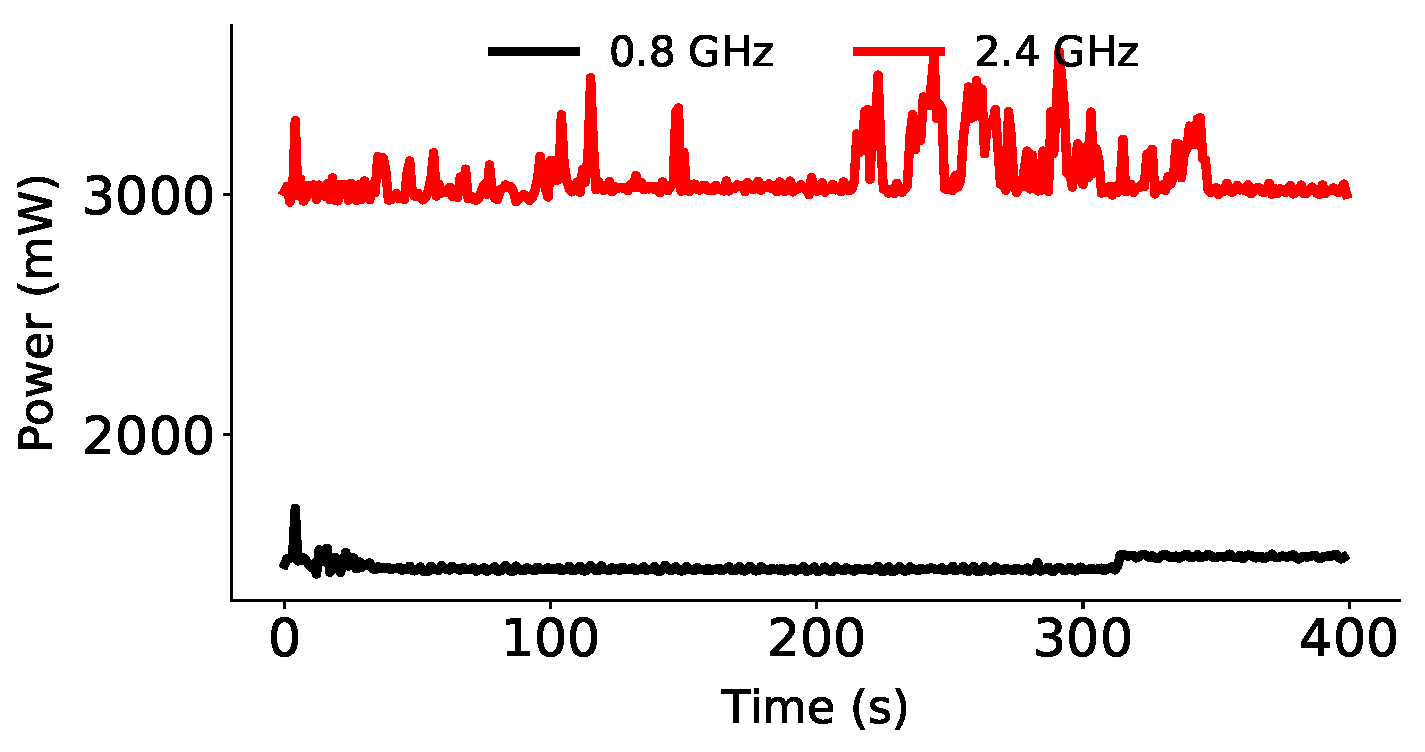
\includegraphics[width=\textwidth]{Chapter3/Figs/trace-files/new/power_orig.eps}
      \caption{Power variation with time.}
      \label{fig: powerastartime}
    \end{subfigure}
    \begin{subfigure}{0.48\textwidth}
      \centering
        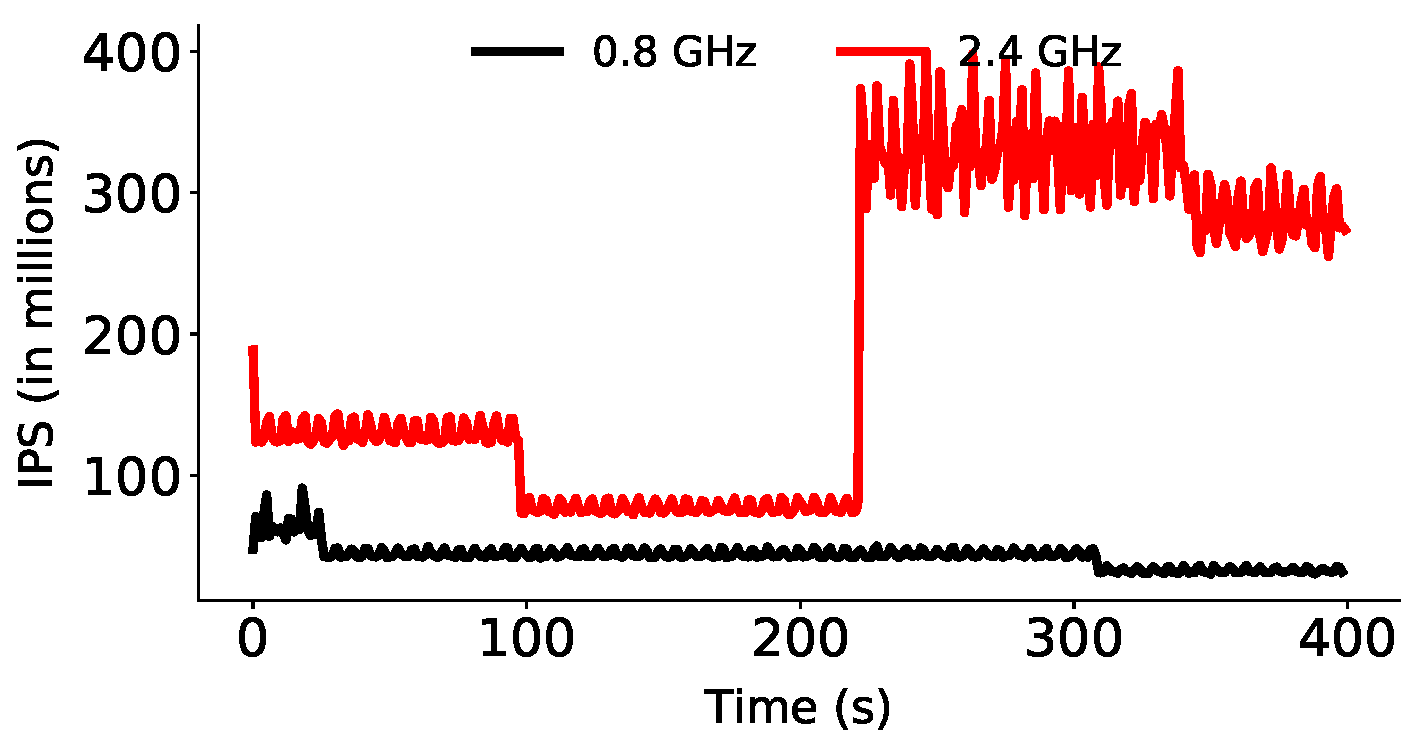
\includegraphics[width=\textwidth]{Chapter3/Figs/trace-files/new/perf_orig.eps}
      \caption{IPS variation with time.}
      \label{fig: perfastartime}
    \end{subfigure} 
    \begin{subfigure}{0.48\textwidth} 
        \centering
        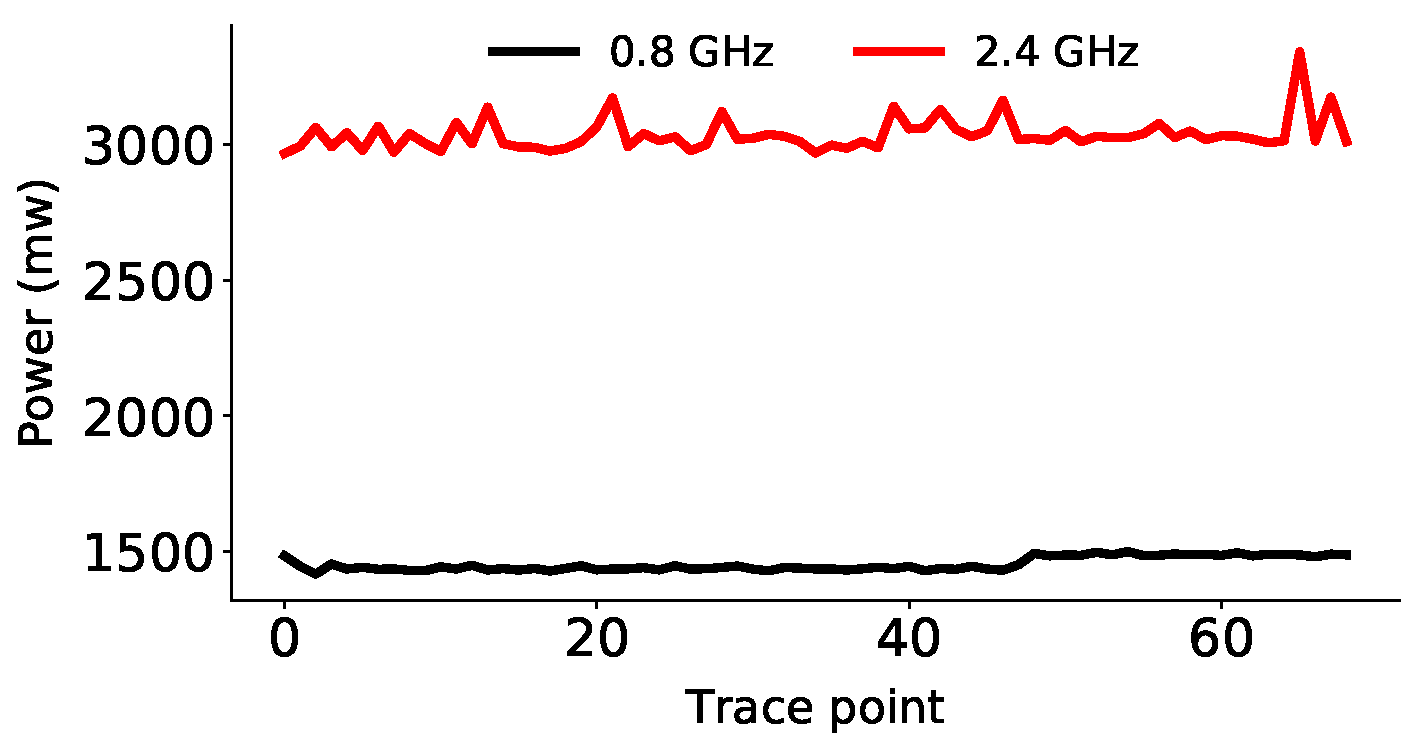
\includegraphics[width=\textwidth]{Chapter3/Figs/trace-files/new/power_realign.eps}
        \caption{Power traces realigned with IPS.} 
        \label{fig: astarpowerrealign}
    \end{subfigure} 
    \begin{subfigure}{0.48\textwidth} 
        \centering
        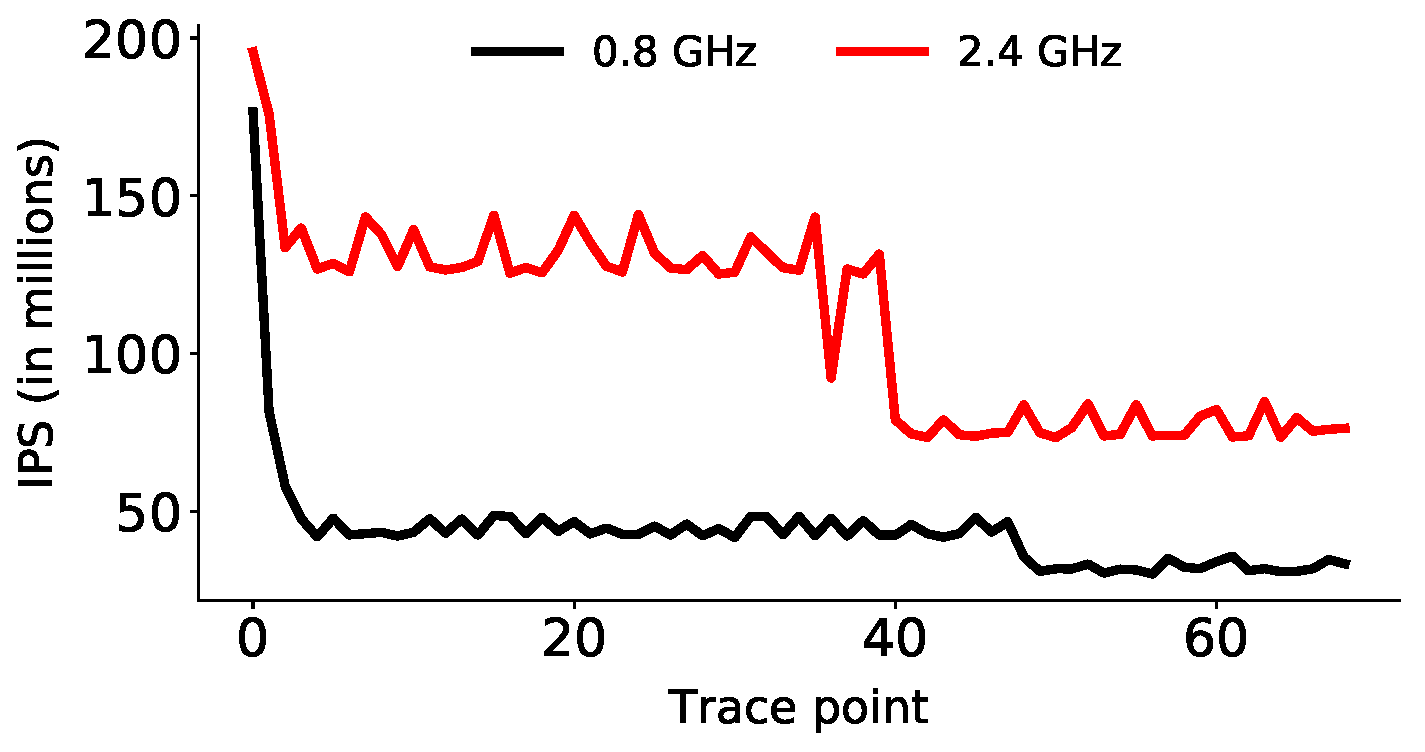
\includegraphics[width=\textwidth]{Chapter3/Figs/trace-files/new/perf_realign.eps}
        \caption{IPS traces realigned with IPS.} 
        \label{fig: astarmipsrealign} 
    \end{subfigure}
    \caption[Traces to build multi linear regression models]{\captitle{Traces to build multi linear regression models.} From
left-to-right, power and performance \textit{recorded} using the power meter and PMCs
(on top), and traces \textit{realigned} based on IPS (on bottom) for the SPEC benchmark
astar.} \label{fig: tracefile-astar} \end{figure} 


The models are built offline using the statistical information gathered and stored in
trace files. The trace files contain activity ratio for individual components for each
benchmark. The traces, obtained at different DVFS states, Cl-States need to be realigned
such that the activity ratios are comparable at similar points of execution. 

\looseness -1 The performance statistics for each benchmark in the training dataset are
gathered by setting a thread affinity to a core using the Linux system call
\texttt{sched\_setaffinity}.  Assigning an affinity~\citep{LinuxKernel} for a thread
bypasses the Linux Completely Fair Scheduler (CFS) and helps avoid excessive thread
migration and provides a more controlled environment.

\looseness -1 Realigning traces gathered at DVFS state, Cl-State to model offline provides
a unique challenge as the correlation between throughput, DVFS state, and  time is
non-linear. For instance, Figures~\ref{fig: powerastartime} and~\ref{fig: perfastartime}
show power consumption (in \SI{}{\milli\watt}) and throughput (in MIPS), respectively, for
SPEC benchmark \emph{astar} at \SI{0.8}{\giga\hertz} (in black) and \SI{2.4}{\giga\hertz}
(in red) with Cl-State zero for the first 400 seconds of execution. For e.g., observe that
the throughput obtained over the first 300 seconds at \SI{0.8}{\giga\hertz}, and first
100-seconds at \SI{2.4}{\giga\hertz} is approximately same. This shows that DVFS state and
throughput do not have a one-to-one mapping.  For this reason, prediction models can not
be built using traces gathered based on a time varying demand of workloads.  This raises
the need to realign traces with respect to performance, thereby allowing (some)
correlation between two different core frequency and performance.

\looseness -1 As indicated before, a buffer of ten million instructions is used to compare
traces for each benchmark, as most SPEC benchmarks exhibit less then \SI{2}{\percent}
difference and to ensure that the boundary of error is fixed (!).  Figures~\ref{fig:
astarpowerrealign} and~\ref{fig: astarmipsrealign} shows the traces realigned with
respect to total performance for \emph{astar} at \SI{0.8}{\giga\hertz} and
\SI{2.4}{\giga\hertz}. Each trace gathered refers to (approximately) similar points of
thread execution. This methodology is followed for every DVFS state and Cl-State
combination, and such traces here-forth are referred to as \emph{\textbf{realigned
traces}}.

\section{Multicore Modelling}
\label{subsec: mult model}

To predict total performance or power in multicore architectures, we \textit{aggregate}
the results from each of the \textit{single-core} models (Section~\ref{subsec: algo}). 

Single-core models when exposed to multicore prediction techniques are bound to suffer
from an error due to the contention for shared
resources~\citep{Blagodurov:2010:CSM:1880018.1880019, Nishtala:2013:ETC:2555754.2555775,
Lefurgy:2008:PCP:1355774.1355779, McCullough:2011:EEM:2002181.2002193,6974701,
Becchi:2006:DTA:1128022.1128029, Gandhi:2010:OAE:1869138.1869264,
Brooks:2000:WFA:339647.339657, Gandhi:2009:OPA:1555349.1555368,6604487}.  
To model the contention when predicting performance and power, we use four different
types of multiprogrammed workloads with variations in memory footprint and validate the
models, by switching between combinations of DVFS states and Cl-States.   

\looseness -1 It impossible to be at two DVFS states or Cl-States at the same time.
Therefore for training and validating the models, we generate multiple (one thousand)
random tuples of DVFS state, Cl-State combinations per core within the minimum and maximum
DVFS state and Cl-State ranges.

The estimated increase in power consumption and degradation in performance due to the
shared resource contention is modelled offline using multi linear regression techniques.
We build one model for performance and another model for power. We demonstrate the process
of building models for one core. This process is replicated across all cores
simultaneously. 

\begin{itemize}

    \item[{\small \circled{1}}] Read the 1000 random tuples of DVFS state and Cl-State per
        core.

    \item[{\small \circled{2}}] Set current configuration for core to the current tuple
        and future configuration for the same core to next tuples.

\item[{\small\circled{3}}] Spawn training workloads consecutively.

\item[{\small\circled{4}}] Apply the single-core algorithm (Section~\ref{subsec: algo})
    for the thread running on the core to predict power and performance in the future
        configuration.

\item[{\small\circled{5}}] Switch to future configuration after \SI{250}{\milli\second}.

\item[{\small\circled{6}}] Report power and performance at future configuration using RAPL
    and PMCs respectively. 

\item[{\small\circled{7}}] Using the PMCs read at current configuration, compute activity
    ratios for private L1, private L2, LLC and MEM for the thread.

\item[{\small\circled{8}}] Compute difference between the PMCs read (or RAPL register) and
    prediction (using REPP) for performance (or power) per thread in the workload models
        the error due to shared resource contention.  

\end{itemize}


The aforementioned method is followed for all random tuples generated for all cores for a
period of 300 seconds. 

\begin{equation}%\tag{Equation 5}
    \label{eq: critical error}
     Error = \sum_{i=0}^{comps}(\Delta_{\mathit{i}} \times AR_{\mathit{i}}) + constant
\end{equation}

Equation~\ref{eq: critical error} represents the multi linear regression model to predict
the error due to shared resource contention. Where $\Delta_{\mathit{i}}$ represents the
coefficient to be learnt and $AR_{\mathit{i}}$ represents the activity ratio of the
individual components. 

Intuitively, in a multicore architecture as the number of threads increases, the
performance per thread decreases and the total power consumption increases. Since the
single-core models do not include contention in shared environments, the total power
consumed will be lower and the performance higher. Therefore, the modelled error for power
and performance is added and subtracted for every prediction on a per thread level
respectively.

    
Then, we evaluate REPP across a wide range of performance and power constraints.  Contrary
to prior works~\citep{Su:2014:POP:2742155.2742200, Cochran:2011:PCA:2155620.2155641,
Singh:2009:RTP:1577129.1577137, Miftakhutdinov:2012:PPI:2457472.2457493, 
Srinivasan:2011:EIO:1945023.1945032}, which predict power and performance at a system
level, our work predicts at a system level on a per core basis.

\begin{figure}[t]
    \centering
    \includegraphics[scale=0.7]{Chapter3/Figs/repp-arch/REPP.pdf}
    \caption{High-level view of REPP runtime system} 
    \label{fig: archrepp} 
\end{figure}


With the inclusion of the shared resource contention model (Equation~\ref{eq: critical
error}), the architecture of REPP for multicore systems is complete. Figure~\ref{fig:
archrepp} shows a high-level view of REPP. REPP is a technique that can be implemented
across any multicore server system running an operating system that allows to gather
performance statistics of workloads (e.g., \textsf{perf}, on all our multicore machines).
Such performance statistics from each thread are fed to REPP to compute the activity
ratio's which are fed to the single-core models to estimate the power and performance
across a wide range of DVFS states and Cl-States. Using equation~\ref{eq: critical error},
we model the shared resource contention  as the single-core models ignore it.  Then, the
results from each of these single-core models are \textit{aggregated} to estimate the
power for a multicore system. 

\newpage

\nomenclature[z-PAAE]{PAAE}{Percentage Absolute Average Error}
\nomenclature[z-STDEV]{STDEV}{Standard Deviation}


\section{Single-Core Model Evaluation} 

In this section, we first introduce the model assessment metric, then we evaluate the
models offline by predicting performance and power using the traces gathered.  Next, we
evaluate the single-core models when predicting performance and power at runtime/online.
Both the evaluations are carried by predicting performance and power from the current DVFS
state, Cl-State to numerous DVFS state and Cl-State combinations. 

\subsection{Model Assessment}
\label{subsubsec: metric}

The models are evaluated in the remainder of this chapter in terms of Percentage Absolute
Average Error (PAAE), and the Standard Deviation (STDEV) for each data point over a period
of 300 seconds:

\begin{equation}
    \label{eq: PAAE}
PAAE = 
\frac{1}{N}\biggl(\,
  \sum_{i=1}^{N}
  \frac{\abs{M_{\mathit{i}} - m_{\mathit{i}}}}
        {m_{\mathit{i}}}
\,\biggr)
\end{equation} 

Where $N$ is the number of data points for each benchmark, $M$ is the predicted value, and
$m$ is the measured value (Reproduced from~\citep{Pusukuri-PAAE}).

The PAAE is a well-known metric~\citep{Su:2014:POP:2742155.2742200, 10.1109/TC.2012.97,
Pusukuri-PAAE, Bircher-PAAE} to evaluate the predicted
performance (or power) values against the actual values reported by PMCs for performance
(or by power monitors for power consumption). The standard deviation over PAAE determines
the variability of PAAE from the actual value.

\subsection{Offline Evaluation} 
\label{subsubsection: offlinesinglecore evaluation}

The offline evaluation of the single-core models is carried out over a subset of DVFS
states and Cl-States. The subset is chosen to represent the spectrum of error variability.
Specifically, the DVFS states chosen are \SI{0.8}{\giga\hertz}, \SI{1.6}{\giga\hertz}, and
\SI{2.4}{\giga\hertz}; and the Cl-States chosen are 0, 30 and 50.

The PAAE is computed as the error between the predicted performance and power at the
future DVFS state and Cl-State using the PMCs obtained at the current DVFS state and
Cl-State for a given number of instructions retired.  The PMCs and power statistics for a
given workload at each DVFS state, Cl-State are obtained from the realigned traces.  The
error is computed over a period of 300 seconds.

\looseness -1 Table~\ref{tab: P--States: PAAE, Standard deviation and Confidence for
SPECcpu2006 benchmarks -- POWER.} shows the power prediction error, in terms of PAAE and
STDEV, when switching from lower to higher DVFS state (left-hand side of the table) and
higher to lower DVFS state (right-hand side of the table) for SPEC workloads.  Our results
have shown that the PAAE over the subset of switches in DVFS states is less than
\SI{2.30}{\percent} (mean), while the maximum error is \SI{5.78}{\percent} for
\emph{soplex}.

\looseness -1 Table~\ref{tab: P--States: PAAE, Standard deviation and Confidence for
SPECcpu2006 benchmarks -- MIPS.} shows the performance prediction error, in terms of PAAE
and STDEV, when switching from lower to higher DVFS state (left-hand side of the table)
and higher to lower DVFS state (right-hand side of the table) for SPEC workloads. The
worst-case scenario PAAE is \SI{33.99}{\percent} for the memory-intensive benchmark
\emph{xalancbmk}.  Also, note that there exists a collinearity between PAAE and the ratio
of change in DVFS state.  For instance, observe there is a linear increase (or decrease)
in PAAE for benchmark \emph{astar} when switching from lower-to-higher (or higher to
lower) DVFS state.

\looseness -1 Table~\ref{tab: Cl--States: PAAE, Standard deviation and Confidence for
SPECcpu2006 benchmarks -- Power.} shows the power prediction error, in terms of PAAE and
STDEV, when switching from lower to higher Cl-State (left-hand side of the table) and
higher to lower Cl-State (right-hand side of the table) at \SI{1.8}{\giga\hertz}.   Our
results have shown that the PAAE over the subset of switches in Cl-State is less than
\SI{4.30}{\percent} (mean), with a maximum error of \SI{10.45}{\percent} for
\emph{xalancbmk}. 

\looseness -1 Table~\ref{tab: Cl--States: PAAE, Standard deviation and Confidence for
SPECcpu2006 benchmarks -- MIPS.} shows the performance prediction error, in terms of PAAE
and STDEV, when switching from lower to higher Cl-State (left-hand side of the table) and
higher to lower Cl-State (right-hand side of the table) at \SI{1.8}{\giga\hertz}.  The
mean error observed when switching between the Cl-States is \SI{15.38}{\percent} (with a
maximum error of \SI{37.77}{\percent} for \emph{calculix}). 

Our results demonstrate that the error across numerous switches, for both DVFS states, and
Cl-States, in an offline modelling technique is ``acceptable''~\citep{Nishtala:2013:ETC:2555754.2555775, 
Su:2014:POP:2742155.2742200, Nishtala:ICPP, Nishtala:SBACPAD, Nishtala:IGSC, Bircher-PAAE}, to determine the real behaviour of the application.  

\looseness -1 Figure~\ref{fig: astarpowerperf} represents the predicted performance
($y$-axis), and power ($x$-axis) for three workloads: \emph{astar} (mid memory intensive;
top row, subfigures (a), (b)), \emph{mcf} (memory intensive; middle row, subfigures (c),
(d)), and \emph{calculix} (compute intensive; bottom row, subfigures (e), (f)). In the
left column, the colour map corresponds to the maximum PAAE between performance, and power
($max_{\mathit{PAAE}}$ = $max$($PAAE_{\mathit{power}}$, $PAAE_{\mathit{performance}}$));
where each point in the graph represents a unique hardware configuration. By contrast, in
the right column, we represent the data plotted in the left column in terms of maximum
error per sub-grid for each benchmark, where a configuration exists. The initial
configuration is set to \SI{0.8}{\giga\hertz} and Cl-State zero. We evaluate the models
offline over nine DVFS states and six Cl-States. These graphs conclude that there exists
at least one prediction with less than \SI{15}{\percent} error. This behaviour was
observed across all SPEC benchmarks.


%%%%%%%%%%%%%%%%%%%%%%%%%%%%%%%%%%%%%%%%%%%%%%%%%%%%%%%%%%%%%%%%%%%%%%%%%%%%%%%
\begin{sidewaystable}
    \sisetup{round-mode=places, round-precision=2}    
\centering
\setlength{\tabcolsep}{3.1pt}

    \caption[Power prediction error across DVFS states]{\captitle{Power prediction error across DVFS states for SPEC benchmarks.} Error shown in terms of PAAE and STDEV. The highest PAAE when predicting across DVFS states is \textbf{boldfaced}.}
\scalebox{1}{
\begin{tabular}{@{}l SSSSSS c@{\hspace{-1em}}  SSSSSS c   @{}}
    \toprule
    & \multicolumn{6}{c}{$\textbf{Lower-Higher}$} & \phantom{abc} & \multicolumn{6}{c}{$\textbf{Higher-Lower}$}\\
    \cmidrule{2-7} \cmidrule{9-14} 
    DVFS state (\SI{}{\giga\hertz})     
    & \multicolumn{2}{c}{\SI{0.8}{} - \SI{1.0}{}} & \multicolumn{2}{c}{\SI{0.8}{} - \SI{1.6}{}} & \multicolumn{2}{c}{\SI{0.8}{} - \SI{2.4}{}} 
    && \multicolumn{2}{c}{\SI{1.0}{} - \SI{0.8}{}} & \multicolumn{2}{c}{\SI{1.6}{} - \SI{0.8}{}} & \multicolumn{2}{c}{\SI{2.4}{} - \SI{0.8}{}}  \\ 

    \cmidrule(r){2-3} \cmidrule(r){4-5} \cmidrule(r){6-7} 
    \cmidrule(r){9-10} \cmidrule(r){11-12} \cmidrule(r){13-14}
    Benchmark & \multicolumn{1}{c}{$PAAE$} & \multicolumn{1}{c}{$STDEV$} & \multicolumn{1}{c}{$PAAE$} & \multicolumn{1}{c}{$STDEV$} & \multicolumn{1}{c}{$PAAE$} & \multicolumn{1}{c}{$STDEV$}
    && \multicolumn{1}{c}{$PAAE$} & \multicolumn{1}{c}{$STDEV$} & \multicolumn{1}{c}{$PAAE$} & \multicolumn{1}{c}{$STDEV$} & \multicolumn{1}{c}{$PAAE$} & \multicolumn{1}{c}{$STDEV$} \\
   %\\\cmidrule[\lightrulewidth](r{\dimexpr5.5cm+\tabcolsep-7.75cm\relax}){1-6}%\addlinespace[1ex] 
    \midrule
    Astar           &1.772&1.282&1.492&0.971&1.172&0.779 &&1.735&0.670&1.718&0.713&2.245&2.580\\ %\hline
    Bzip2           &1.927&0.945&1.922&2.482&1.401&0.981 &&1.136&0.679&0.824&0.525&2.053&1.727\\ %\hline
    Calculix        &1.267&1.195&1.274&1.133&3.480&2.098 &&1.114&0.572&2.371&2.245&2.356&2.042\\ %\hline
    GemsFDTD        &3.882&2.773&3.541&2.127&4.238&2.303 &&3.739&2.952&3.781&2.241&3.357&1.704\\ %\hline
    Gobmk           &1.054&0.940&1.339&1.605&2.409&3.201 &&0.856&0.652&0.697&0.466&0.665&0.572\\ %\hline
    Hmmer           &2.600&0.528&2.523&0.861&3.062&1.452 &&2.738&0.618&2.696&0.598&2.307&0.927\\ %\hline
    Lbm             &0.849&0.686&1.824&1.101&2.155&1.380 &&0.840&0.697&1.431&0.825&1.473&0.771\\ %\hline
    Leslie3d        &1.095&0.862&1.324&1.283&2.036&1.200 &&1.240&0.958&1.165&0.931&1.377&1.233\\ %\hline
    Libquantum      &2.676&3.906&1.643&1.255&2.435&1.953 &&3.330&2.766&1.957&1.496&1.852&1.852\\ %\hline
    Mcf             &3.172&2.355&3.785&2.677&5.666&2.249 &&2.419&2.656&2.292&2.227&2.422&2.724\\ %\hline
    Povray          &1.143&0.615&2.049&1.093&1.897&3.250 &&1.234&0.514&1.396&0.546&1.060&0.466\\ %\hline
    Soplex          &5.132&1.722&2.761&1.629&2.816&1.163 &&  \textbf{5.78}  &1.988&5.687&1.880&4.135&1.706\\ %\hline
    Xalancbmk       &2.522&1.587&3.627&1.580&5.807&1.457 &&1.986&1.358&1.617&1.154&1.401&1.242\\ %\hline
    {\bf Mean}      &2.238&1.492&2.239&1.523&2.967&1.805 &&2.165&1.314&2.126&1.219&2.054&1.504\\ 
\bottomrule
\end{tabular}
}
\label{tab: P--States: PAAE, Standard deviation and Confidence for SPECcpu2006 benchmarks -- POWER.}
\end{sidewaystable}


\begin{sidewaystable}%table*}[t]
    \sisetup{round-mode=places, round-precision=2}    
\centering
\setlength{\tabcolsep}{3.1pt}
    \caption[Performance prediction error across DVFS states]{\captitle{Performance prediction error across DVFS states for SPEC benchmarks.} Error shown in terms of PAAE and STDEV. The highest PAAE when predicting across DVFS states is \textbf{boldfaced}.}
\scalebox{1}{
\begin{tabular}{@{}l SSSSSS c@{\hspace{-0.9em}}  SSSSSS c   @{}}
    \toprule
    & \multicolumn{6}{c}{$\textbf{Lower-Higher}$} & \phantom{abc} & \multicolumn{6}{c}{$\textbf{Higher-Lower}$}\\
    \cmidrule{2-7} \cmidrule{9-14} 
    DVFS state (\SI{}{\giga\hertz})     
    & \multicolumn{2}{c}{\SI{0.8}{} - \SI{1.0}{}} & \multicolumn{2}{c}{\SI{0.8}{} - \SI{1.6}{}} & \multicolumn{2}{c}{\SI{0.8}{} - \SI{2.4}{}} 
    && \multicolumn{2}{c}{\SI{1.0}{} - \SI{0.8}{}} & \multicolumn{2}{c}{\SI{1.6}{} - \SI{0.8}{}} & \multicolumn{2}{c}{\SI{2.4}{} - \SI{0.8}{}}  \\ 
    \cmidrule(r){2-3} \cmidrule(r){4-5} \cmidrule(r){6-7} 
    \cmidrule(r){9-10} \cmidrule(r){11-12} \cmidrule(r){13-14}
    Benchmark & \multicolumn{1}{c}{$PAAE$} & \multicolumn{1}{c}{$STDEV$} & \multicolumn{1}{c}{$PAAE$} & \multicolumn{1}{c}{$STDEV$} & \multicolumn{1}{c}{$PAAE$} & \multicolumn{1}{c}{$STDEV$}
    && \multicolumn{1}{c}{$PAAE$} & \multicolumn{1}{c}{$STDEV$} & \multicolumn{1}{c}{$PAAE$} & \multicolumn{1}{c}{$STDEV$} & \multicolumn{1}{c}{$PAAE$} & \multicolumn{1}{c}{$STDEV$} \\
    \midrule
    Astar       &9.409 &16.745 &11.174&14.054 &24.076 &9.518   &&7.923 &8.647   &9.126 &9.41     &16.242&14.443 \\ %\hline
    Bzip2       &13.163&11.362 &17.277&11.752 &22.979 &15.542  &&13.061&10.495  &19.802&17.591   &22.663&13.478 \\ %\hline
    Calculix    &22.19 &13.435 &19.24 &15.115 &26.968 &20.412  &&17.219 &26.997  &18.165&24.183   &19.888&23.932 \\ %\hline
    GemsFDTD    &21.687&15.48  &23.884&14.5   &15.65  &14.648  &&21.707&15.58   &22.433&12.316   &12.709&9.618  \\ %\hline
    Gobmk       &8.968 &7.824  &8.742 &8.686  &9.236  &7.158   &&8.852 &7.607   &8.889 &9.119    &9.614&8.045  \\ %\hline
    H264ref     &6.095 &4.689  &9.177 &14.613 &1.887  &1.353   &&6.116 &4.707   &7.705 &8.513    &1.94&1.42    \\ %\hline
    Hmmer       &5.704 &5.982  &6.088 &5.342  &6.999  &4.742   &&5.985 &7.567   &6.136 &5.337    &7.434&5.26   \\ %\hline
    Lbm         &6.931 &5.103  &5.824 &4.122  &5.773  &3.866   &&6.843 &4.984   &5.734 &4.009    &5.629&3.771  \\ %\hline
    Libquantum  &8.602 &6.359  &10.3  &7.095  &12.577 &10.284  &&8.635 &6.521   &9.545 &6.445    &10.541&7.697 \\ %\hline
    Mcf         &11.081&9.698  &17.721&15.106 &29.327 &20.954  &&10.441&9.11    &14.672&12.777   &21.431&11.328\\ %\hline
    Povray      &6.15  &4.415  &12.09 &22.553 &6.932  &5.114   &&6.241 &4.673   &9.145 &10.637   &7.121&5.42   \\ %\hline
    Soplex      &8.829 &6.744  &10.344&8.555  &16.778 &13.797  &&8.192 &5.758   &9.039 &6.553    &13.366&8.671 \\ %\hline
    Xalancbmk   &9.653 &8.565  &19.31 &13.979 &\textbf{33.99} &16.745  &&9.702 &9.427   &15.461&9.203    &25.172&11.007\\ %\hline
    {\bf Mean}  &10.651&8.954  &13.167&11.959 &16.398 &11.087  &&10.071&9.390   &11.989&10.469   &13.365&9.545  \\ 
\bottomrule
\end{tabular}
}
\label{tab: P--States: PAAE, Standard deviation and Confidence for SPECcpu2006 benchmarks -- MIPS.}
\end{sidewaystable}





\begin{sidewaystable}%table*}[t]
    \sisetup{round-mode=places, round-precision=2}    
\centering
\setlength{\tabcolsep}{3.1pt}
    \caption[Power prediction error when switching across Cl-States at \SI{1.8}{\giga\hertz}]{\captitle{Power prediction error when switching across Cl-States at \SI{1.8}{\giga\hertz} for SPEC benchmarks.} Error shown in terms of PAAE and STDEV. The highest PAAE when predicting across Cl-States is \textbf{boldfaced}.}
\scalebox{1}{
\begin{tabular}{@{}l SSSSSS c@{\hspace{-0.9em}}  SSSSSS c   @{}}
    \toprule
    & \multicolumn{6}{c}{$\textbf{Lower-Higher}$} & \phantom{abc} & \multicolumn{6}{c}{$\textbf{Higher-Lower}$}\\
    \cmidrule{2-7} \cmidrule{9-14} 
    Cl-State    & \multicolumn{2}{c}{$0-10$} & \multicolumn{2}{c}{$0-30$} & \multicolumn{2}{c}{$0-50$} && \multicolumn{2}{c}{$10-0$} & \multicolumn{2}{c}{$30-0$} & \multicolumn{2}{c}{$50-0$}  \\ 
    \cmidrule(r){2-3} \cmidrule(r){4-5} \cmidrule(r){6-7} 
    \cmidrule(r){9-10} \cmidrule(r){11-12} \cmidrule(r){13-14}
    Benchmark & \multicolumn{1}{c}{$PAAE$} & \multicolumn{1}{c}{$STDEV$} & \multicolumn{1}{c}{$PAAE$} & \multicolumn{1}{c}{$STDEV$} & \multicolumn{1}{c}{$PAAE$} & \multicolumn{1}{c}{$STDEV$}
    && \multicolumn{1}{c}{$PAAE$} & \multicolumn{1}{c}{$STDEV$} & \multicolumn{1}{c}{$PAAE$} & \multicolumn{1}{c}{$STDEV$} & \multicolumn{1}{c}{$PAAE$} & \multicolumn{1}{c}{$STDEV$} \\
    \midrule
    Astar       &3.190&2.308&2.686&1.748&2.110&1.402 &&3.123&1.206 &3.092&1.283 &4.041&4.644 \\ %\hline
    Bzip2       &3.469&1.701&3.460&4.468&2.522&1.766 &&2.045&1.222 &1.483&0.945 &3.695&3.109\\ %\hline
    Calculix    &2.281&2.151&2.293&2.039&6.264&3.776 &&2.005&1.030 &4.268&4.041 &4.241&3.676\\ %\hline
    GemsFDTD    &6.988&4.991&6.374&3.829&7.628&4.145 &&6.730&5.314 &6.806&4.034 &6.043&3.067\\ %\hline
    Gobmk       &1.897&1.692&2.410&2.889&4.336&5.762 &&1.541&1.174 &1.255&0.839 &1.197&1.030\\ %\hline
    Hmmer       &4.680&0.950&4.541&1.550&5.512&2.614 &&4.928&1.112 &4.853&1.076 &4.153&1.669\\ %\hline
    Lbm         &1.528&1.235&3.283&1.982&3.879&2.484 &&1.512&1.255 &2.576&1.485 &2.651&1.388\\ %\hline
    Leslie3d    &1.971&1.552&2.383&2.309&3.665&2.160 &&2.232&1.724 &2.097&1.676 &2.479&2.219\\ %\hline
    Libquantum  &4.817&7.031&2.957&2.259&4.383&3.515 &&5.994&4.979 &3.523&2.693 &3.334&3.334\\ %\hline
    Mcf         &5.710&4.239&6.813&4.819&10.199&4.046&&4.354&4.781&4.126&4.009 &4.360&4.903\\ %\hline
    Povray      &2.057&1.107&3.688&1.967&3.415&5.850 &&2.221&0.925 &2.513&0.983 &1.908&0.839\\ %\hline
    Soplex      &9.238&3.100&4.970&2.932&5.069&2.093 &&10.395&3.578&10.237&3.384&7.443&3.071\\ %\hline
    Xalancbmk   &4.540&2.857&6.529&2.844&\textbf{10.45}&2.623&&3.575&2.444&2.911&2.077 &2.522&2.236\\ %\hline
    {\bf Mean}  &4.028&2.686&4.030&2.741&5.341&3.249 &&3.897&2.365 &3.826&2.194 &3.697&2.707\\ 
\bottomrule
\end{tabular}
}
\label{tab: Cl--States: PAAE, Standard deviation and Confidence for SPECcpu2006 benchmarks -- Power.}
\end{sidewaystable}%table*}

%%%%%%%%%%%%%%%%%%%%%%%%%%%%%%%%%%%%%%%%%%%%%%%%%%%%%%%%%%%%%%%%%%%%%%%%%%%%%%%




\begin{sidewaystable}%table*}[htbp]
    \sisetup{round-mode=places, round-precision=2}    
\centering
\setlength{\tabcolsep}{3.1pt}
    \caption[Performance prediction error when switching across Cl-States at \SI{1.8}{\giga\hertz}]{\captitle{Performance error when switching across Cl-States at \SI{1.8}{\giga\hertz} for SPEC benchmarks.} Error shown in terms of PAAE and STDEV.  The highest PAAE when predicting across Cl-States is \textbf{boldfaced}}
\scalebox{1}{
\begin{tabular}{@{}l SSSSSS c@{\hspace{-0.9em}}  SSSSSS c   @{}}
    \toprule
    & \multicolumn{6}{c}{$\textbf{Lower-Higher}$} & \phantom{abc} & \multicolumn{6}{c}{$\textbf{Higher-Lower}$}\\
    \cmidrule{2-7} \cmidrule{9-14} 
    Cl-State    & \multicolumn{2}{c}{$0-10$} & \multicolumn{2}{c}{$0-30$} & \multicolumn{2}{c}{$0-50$} && \multicolumn{2}{c}{$10-0$} & \multicolumn{2}{c}{$30-0$} & \multicolumn{2}{c}{$50-0$}  \\ 
    \cmidrule(r){2-3} \cmidrule(r){4-5} \cmidrule(r){6-7} 
    \cmidrule(r){9-10} \cmidrule(r){11-12} \cmidrule(r){13-14}
    Benchmark & \multicolumn{1}{c}{$PAAE$} & \multicolumn{1}{c}{$STDEV$} & \multicolumn{1}{c}{$PAAE$} & \multicolumn{1}{c}{$STDEV$} & \multicolumn{1}{c}{$PAAE$} & \multicolumn{1}{c}{$STDEV$}
    && \multicolumn{1}{c}{$PAAE$} & \multicolumn{1}{c}{$STDEV$} & \multicolumn{1}{c}{$PAAE$} & \multicolumn{1}{c}{$STDEV$} & \multicolumn{1}{c}{$PAAE$} & \multicolumn{1}{c}{$STDEV$} \\
    \midrule
    Astar       &9.836 &9.799 &12.440&8.439  &23.711&11.462&&9.394&7.750  &11.462&8.602 &13.588&11.935 \\ %\hline
    Bzip2       &12.486&8.747 &19.400&12.959 &28.110&16.538&&12.847&10.342&19.678&11.790&23.965&19.870\\ %\hline
    Calculix    &23.681&12.9840&17.184&16.378&\textbf{37.77}&22.141&&17.679&14.590&19.893&8.623 &23.289&6.008 \\ %\hline
    GemsFDTD    &17.164&14.747&15.109&9.980  &24.321&16.465&&16.932&15.113&15.312&11.467&23.785&17.364\\ %\hline
    Gobmk       &9.290 &5.734 &12.157&8.156  &24.456&11.360&&9.499&5.947  &11.563&7.668 &14.496&10.778\\ %\hline
    H264ref     &10.302&5.408 &10.646&10.863 &25.193&12.028&&10.669&6.161 &12.767&8.660 &15.129&9.913 \\ %\hline
    Hmmer       &7.408 &4.300 &10.465&6.956  &24.085&12.732&&7.382&4.372  &8.186&6.064  &16.058&10.183\\ %\hline
    Lbm         &10.238&5.787 &12.015&7.584  &25.261&12.579&&10.339&6.474 &11.138&7.127 &15.771&13.232\\ %\hline
    Libquantum  &8.857 &6.154 &12.238&10.852 &24.808&12.907&&8.865&5.854  &13.729&12.958&14.651&10.185\\ %\hline
    Mcf         &9.689 &7.396 &15.263&10.717 &27.495&13.709&&10.650&9.180 &14.185&18.806&19.416&21.161\\ %\hline
    Povray      &8.500 &5.055 &9.751&8.519   &23.424&10.504&&8.718&5.406  &11.298&8.313 &12.902&6.855 \\ %\hline
    Soplex      &7.855 &5.257 &13.407&8.983  &25.487&14.176&&7.972&5.204  &12.413&7.405 &17.496&16.825\\ %\hline
    Xalancbmk   &9.528 &7.612 &10.698&9.382  &31.952&15.761&&9.000&6.764  &11.377&11.185&14.587&8.897 \\ %\hline
    {\bf Mean}      &11.141&7.614 &13.136&9.982  &26.621&14.028&&10.765&7.935 &13.308&9.898 &17.318&12.554\\ 
\bottomrule
\end{tabular}
}
\label{tab: Cl--States: PAAE, Standard deviation and Confidence for SPECcpu2006 benchmarks -- MIPS.}
\end{sidewaystable}%table*}

\begin{figure}[htbp]
    \centering
    \begin{subfigure}{0.48\textwidth}
        \centering
        %\includegraphics[width=\textwidth]{Chapter3/Figs/checkered/astar-power-perf.eps}
        \begin{overpic}[width=\linewidth]{Chapter3/Figs/checkered/astar-power-perf.eps}
            \put(20,85) {\large Prediction error}
            \put(-10,35) {\rotatebox{90}{\large Astar}}
        \end{overpic}
        \caption{\emph{Astar}}
        \label{fig: astar2d}
    \end{subfigure}
    \begin{subfigure}{.48\textwidth} 
        \centering
        %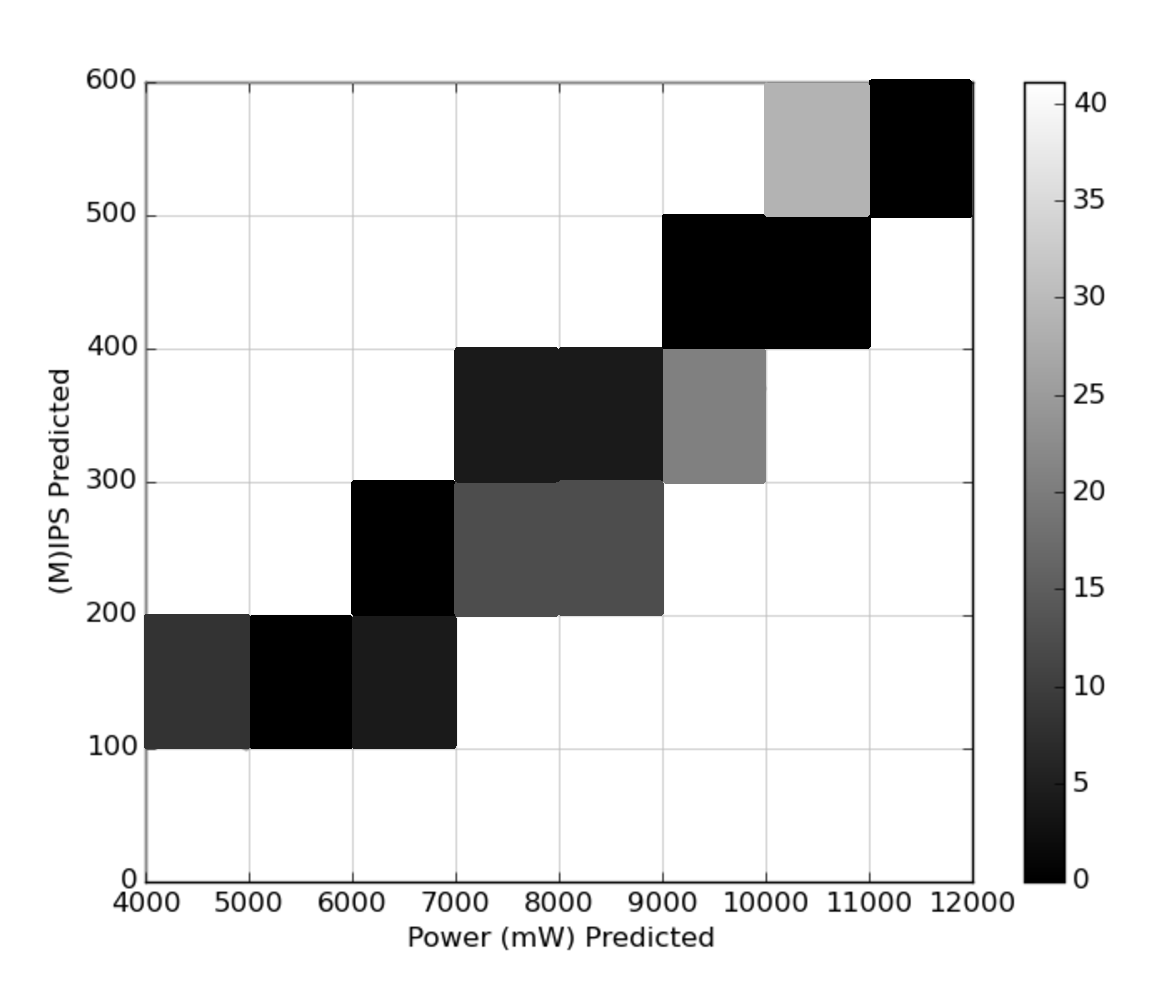
\includegraphics[width=\textwidth]{Chapter3/Figs/checkered/astar-error.eps}
        \begin{overpic}[width=\linewidth]{Chapter3/Figs/checkered/astar-error.eps}
            \put(15, 85) {\large Prediction error per grid}
        \end{overpic}
        \caption{\emph{Astar}}
        \label{fig: astarcheck}
    \end{subfigure}
    \begin{subfigure}{.48\textwidth}
        \centering
        %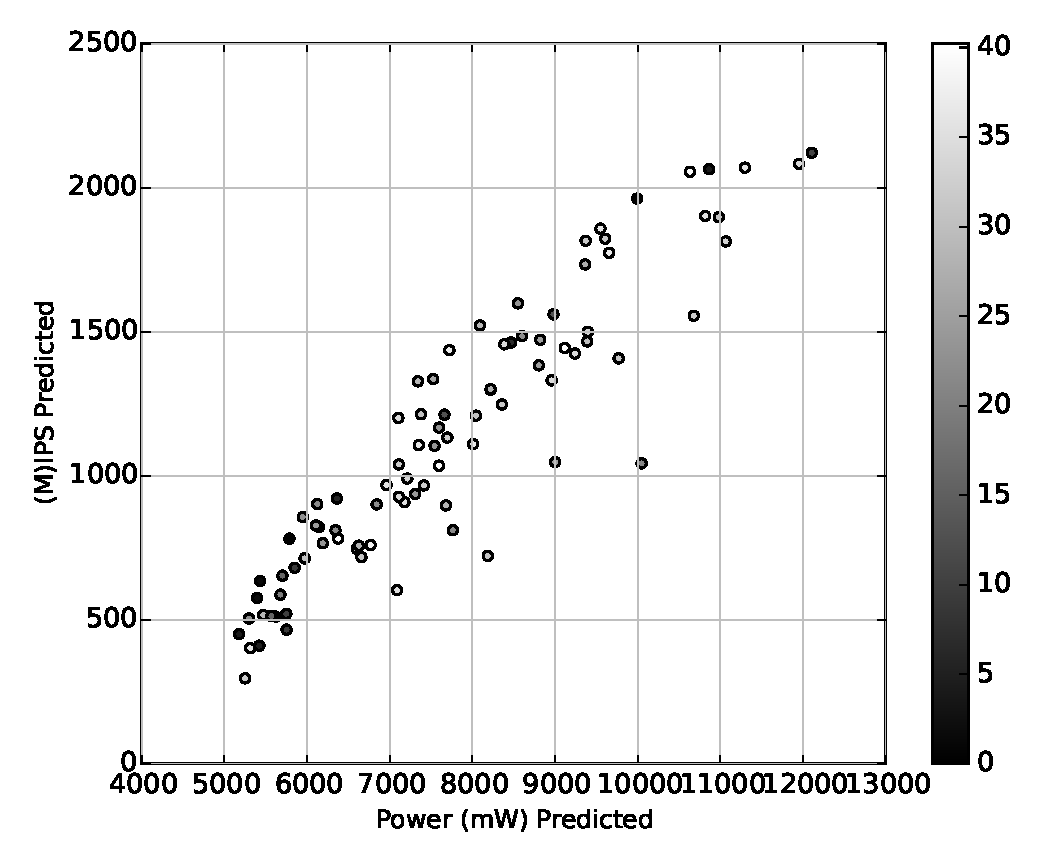
\includegraphics[width=\textwidth]{Chapter3/Figs/checkered/calculix-power-perf.eps}
        \begin{overpic}[width=\linewidth]{Chapter3/Figs/checkered/calculix-power-perf.eps}
        \put(-10,35) {\rotatebox{90}{\large Calculix}}
        \end{overpic}
        \caption{\emph{Calculix}}
        \label{fig: calculix2d}
    \end{subfigure}%
    \begin{subfigure}{.48\textwidth}
        \centering
        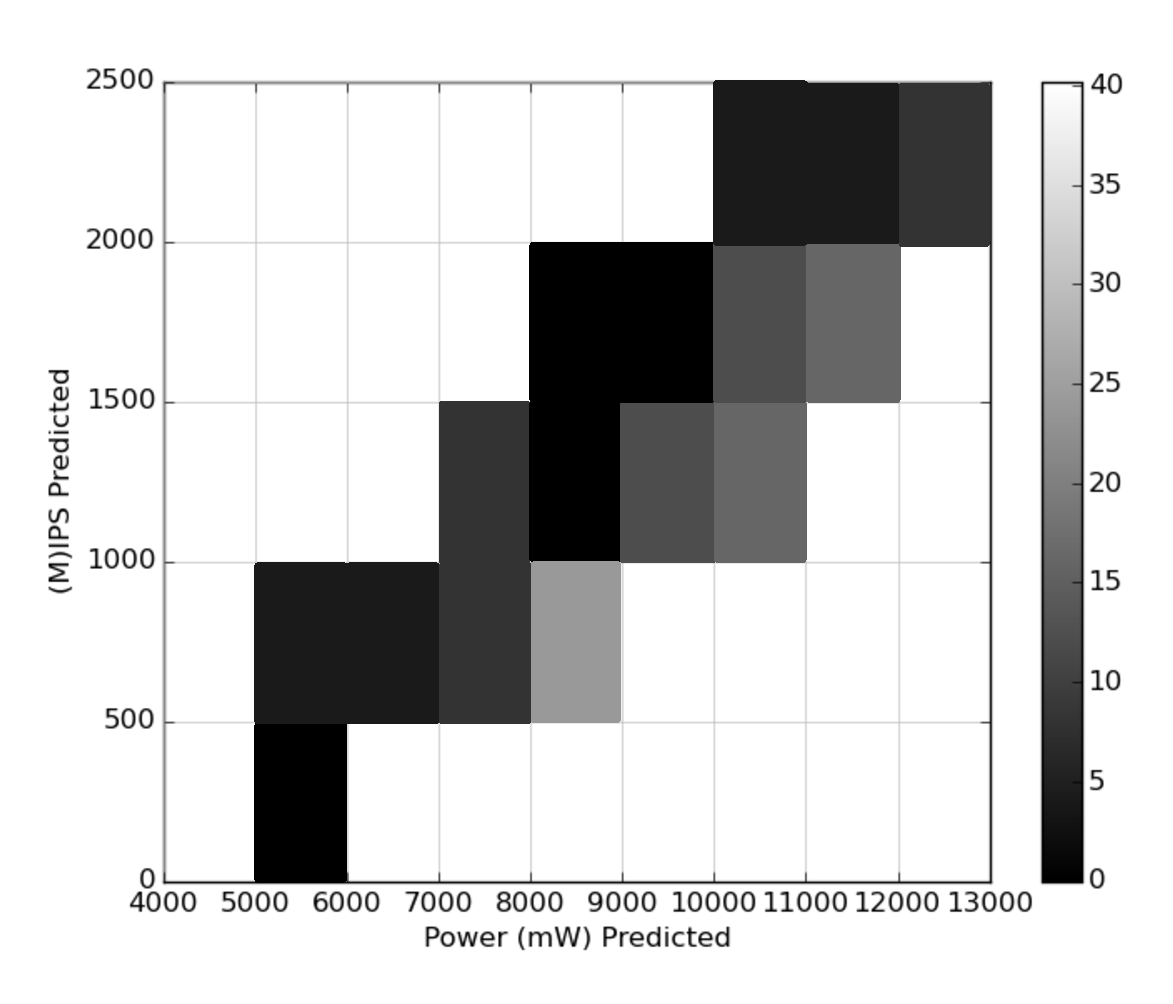
\includegraphics[width=\textwidth]{Chapter3/Figs/checkered/Calculix-error.eps}
        \caption{\emph{Calculix}}
        \label{fig: calculixcheck}
    \end{subfigure}
    \begin{subfigure}{.48\textwidth}
        \centering
        %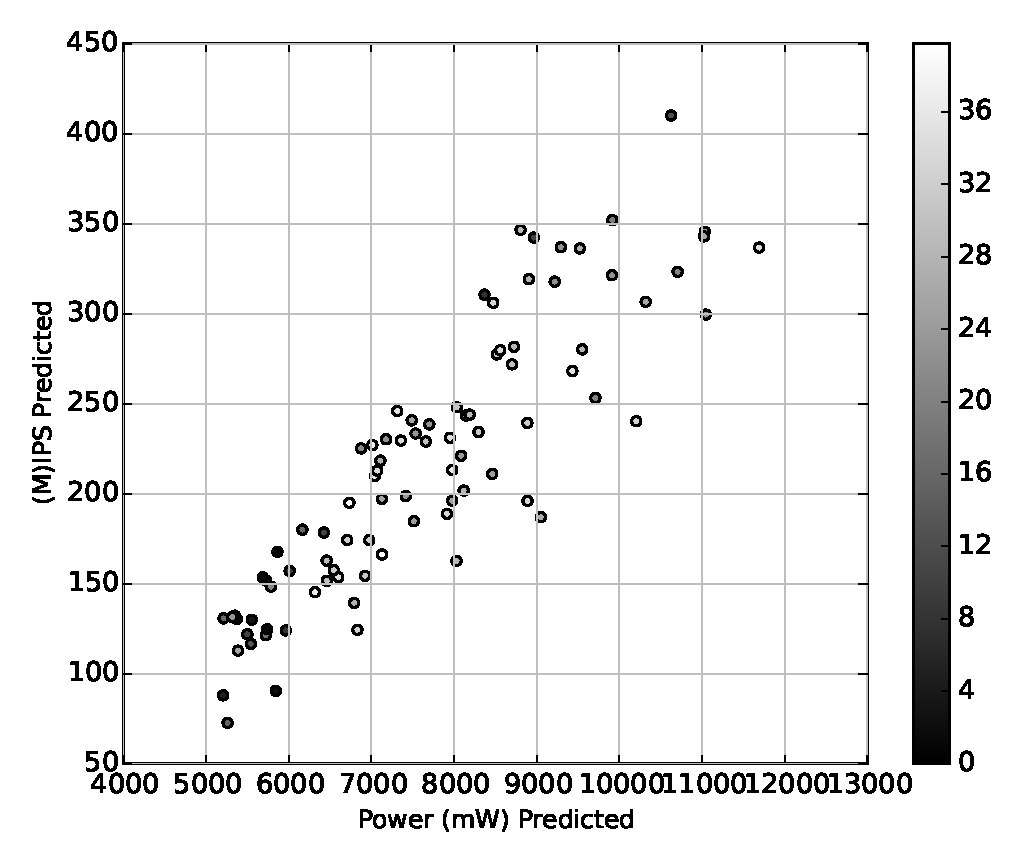
\includegraphics[width=\textwidth]{Chapter3/Figs/checkered/mcf-power-perf.eps}
        \begin{overpic}[width=\linewidth]{Chapter3/Figs/checkered/mcf-power-perf.eps}
        \put(-10,35) {\rotatebox{90}{\large Mcf}}
        \end{overpic}
        \caption{\emph{Mcf}}
        \label{fig: mcf2d}
    \end{subfigure}
    \begin{subfigure}{.48\textwidth}
        \centering
        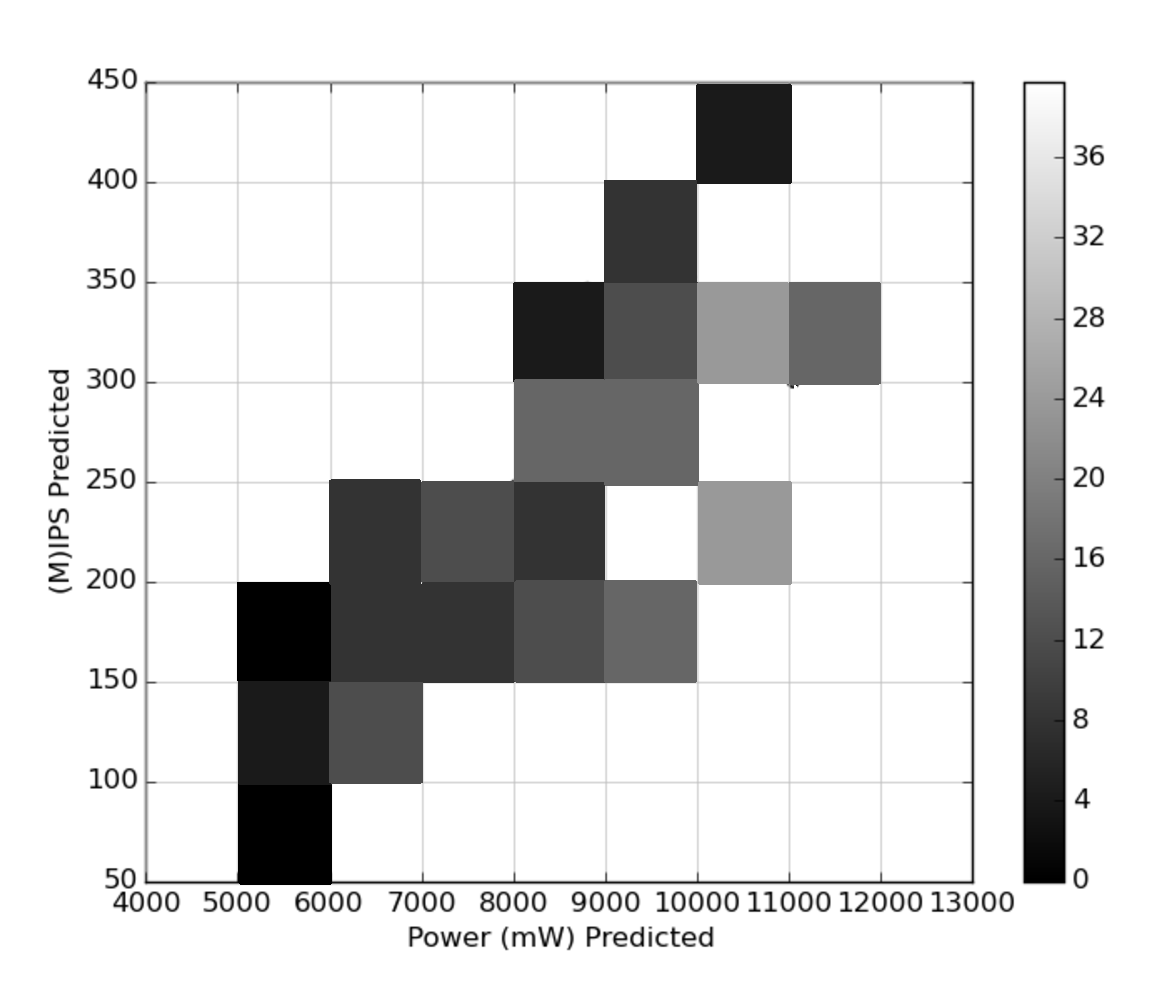
\includegraphics[width=\textwidth]{Chapter3/Figs/checkered/mcf-error.eps}
        \caption{\emph{Mcf}}
        \label{fig: mcfcheck}
    \end{subfigure}

    \caption[Percentage prediction error for SPEC benchmarks]{\captitle{Percentage prediction error for SPEC benchmarks.}  The power and performance prediction error for Astar (mid memory intensive), Calculix (compute intensive), and Mcf (memory intensive).}
        \label{fig: astarpowerperf} 

\end{figure}

\newpage

\subsection{Online Evaluation} 
\label{subsubsection: singlecore eval}  

We evaluate and summarise the single-core modelling technique at runtime for over 150
applications using \textsf{K-Means} clustering algorithm~\citep{Kanungo00anefficient}.
The evaluation is carried out by predicting performance and power across combinations
of DVFS state and Cl-State at runtime. The PAAE on a single-core is computed using the error
between the value measured from PMCs for performance (and power meters for power) and
predicted performance (or power), and the error bars represent the STDEV. 


%\texttt{/home/nishtala/Dropbox/UPC/PhD-Thesis/Chapter3/Figs/single-core-online/separate/} \\
%..make a grid with it. use commented code to build the stuff}

First, we separate the benchmarks used in validation into four \textsf{clusters}, to
present the results for over 150 single-threaded applications, using K-Means with
parameters FE, INT, FP, MEM, BPU, L1, L2, and L3. The number of clusters (four) was chosen
empirically based on the silhouette coefficient. We narrow the number of parameters to two
using principal component analysis for keeping the most singular vectors to project the
data in a lower dimensional space. Clusters are named with the architecture and cluster
number, such as ARM-0, Intel-3, etc. Each cluster has results from all four categories:
Insensitive, Cache-Friendly, Cache-Sensitive, and Thrashing. The benchmarks in each
category are given in Table~\ref{tab: classes}.

\begin{figure}[b]
    \centering
    \includegraphics[width=\textwidth]{Chapter3/Figs/single-core-online/SBAC-PAD/Singlecore-cal.pdf}
    \caption[Average PAAE when predicting performance and power on a single-core]{\captitle{Average PAAE when predicting performance and power on a single-core.} Average PAAE when predicting performance and power on a single-core for across a combination of DVFS states, Cl-States and architectures. The error bars represent the STDEV.}
    \label{fig: singlecore eval}
\end{figure}

Figure~\ref{fig: singlecore eval} shows the average PAAE over-all applications in a
cluster on a single-core and Figure~\ref{fig: singlecoredetail} presents the results for
each application in detail on a single-core. The results in the Figure~\ref{fig:
singlecoredetail} are organised as follows: Intel (top row (a)), AMD (middle row (b)), and
ARM (bottom row (c)). We analyse the data points with higher error and also pointed
out the sources of error below.

{\small \circled{a}} Average PAAE when predicting performance for Intel-2 for
\textit{thrashing} benchmarks is \SI{15.8}{\percent} because \emph{mcf} has
\SI{22.5}{\percent} error as it is a pointer-chasing benchmark~\citep{2006core2} and
generates more than 41000 LLC misses per million instructions retired and the models are
not trained for that range. On the other hand, applications like \emph{lbm} (a memory
intensive floating point benchmark) generate 3000 LLC misses per million instruction
retired has an error \SI{11.2}{\percent}.

{\small \circled{b}} The average PAAE for performance for \textit{Cache-Friendly} on AMD-0 and
AMD-1 are \SI{12.4}{\percent} and \SI{12.3}{\percent}, respectively; this is because both
clusters  contain applications such as \emph{canneal} and \emph{dedup}. The possible
sources of error are: {\small \circled{1}} Both applications have a high dynamic
variability in application phases~\citep{marc}, which leads to erroneous counters due to
PMCs multiplexing. {\small \circled{2}} In contrast to the other applications across
suites, these benchmarks have a shorter execution time. {\small \circled{3}} Observe that
canneal is a cache fitting benchmark on Intel, by contrast it is a cache-friendly
benchmark on AMD. This is because of the aggressive hardware prefetcher on Intel causing a
higher miss rate~\citep{Kang:2013:HPP:2499368.2451155}, thereby leading to fewer dynamic
phase changes and relatively smaller error of \SI{6.5}{\percent}. 

We also observe that application \emph{radix} is a cache-fitting, integer radix sorting
algorithm, has very high activity in FE, across three different architectures, even though
other benchmarks across four suites do not show this behaviour. 

\begin{figure}[b]
    \centering
    \includegraphics[width=\textwidth]{Chapter3/Figs/single-core-online/SBAC-PAD/Cal-Summary.pdf}
    \caption[Average PAAE when predicting performance and power per benchmark suite on a single-core]{\captitle{Average PAAE when predicting performance and power per benchmark on a single-core.} The error bars represent the STDEV.}
    \label{fig: singlecore per suite}
\end{figure}


Figure \ref{fig: singlecore per suite} shows average PAAE over all applications in each
benchmark suite across architectures, with error bars representing STDEV. Across
architectures, we observe performance PAAE is higher for SPEC benchmarks, which have high
variability at runtime, and low for NAS benchmarks, which have less variability after the
initialisation phase. We conclude that the models to predict performance and power are
accurate enough to capture the real behaviour, and since the computational complexity at
runtime is low, they can be used for fine-grain power or performance management. The
models to predict power can be built using standardised power meters and the models are
built using PMCs that are available across architectures.


\begin{table}[t]
    \centering
    \caption[PAAE over combinations of DVFS states and Cl-States using REPP.]{\captitle{PAAE over combinations of DVFS states and Cl-States.} PAAE when predicting performance for every combination of switch in DVFS state and for a specific set of differences when switching between Cl-States for a single-core Intel architecture. Similar results were observed across AMD, and ARM.}
    \scalebox{0.95}{
        \begin{tabular}{@{}lrrrrrrrrr@{}}
        \toprule
        Leap in DVFS State &       1&      2&      3&      4&      5&      6&      7&     8 & -    \\ 
        % \midrule
        DVFS state  & 14.14& 16.75 & 23.37 & 15.37 & 13.78 & 57.17 & 18.49 & 27.49 & -  \\
        \midrule
        Leap in Cl-State&     5   &     10&     15&     20&     25&     30&     35&     40&  45 \\
        % \midrule
        Cl-State &  24.86 & 26.25 & 29.14 & 26.36 & 23.25 & 22.07 & 29.30 & 31.94 & 34.56\\ 
        \bottomrule
        \end{tabular} 
    }
    \label{tab: tabulated perf error}
\end{table}

\looseness -1 Also, we observe that when predicting performance at the future DVFS state
on Intel processors, the error varies depending on the leap size between current DVFS
state to future DVFS state or current Cl-State to future Cl-State.  We compute PAAE when
switching between every combination of DVFS states.  For every switch in DVFS state, we
calculate the PAAE when switching between every combination of DVFS states.  Similarly, we
calculate the PAAE for Cl-States when the difference in switches is a multiple of five for
every DVFS state.  As can be seen in Table~\ref{tab: tabulated perf error}, with a higher
switch in hardware configurations from the current configuration, a greater error is
observed. This is because, we train the models using a small subset of benchmarks, and use
it for a broad range of threads which are not a part of the training set. Similar results
were observed across ARM and AMD machines.


\begin{figure}[H]
\begin{subfigure}[t]{\textwidth}
    \centering        
    %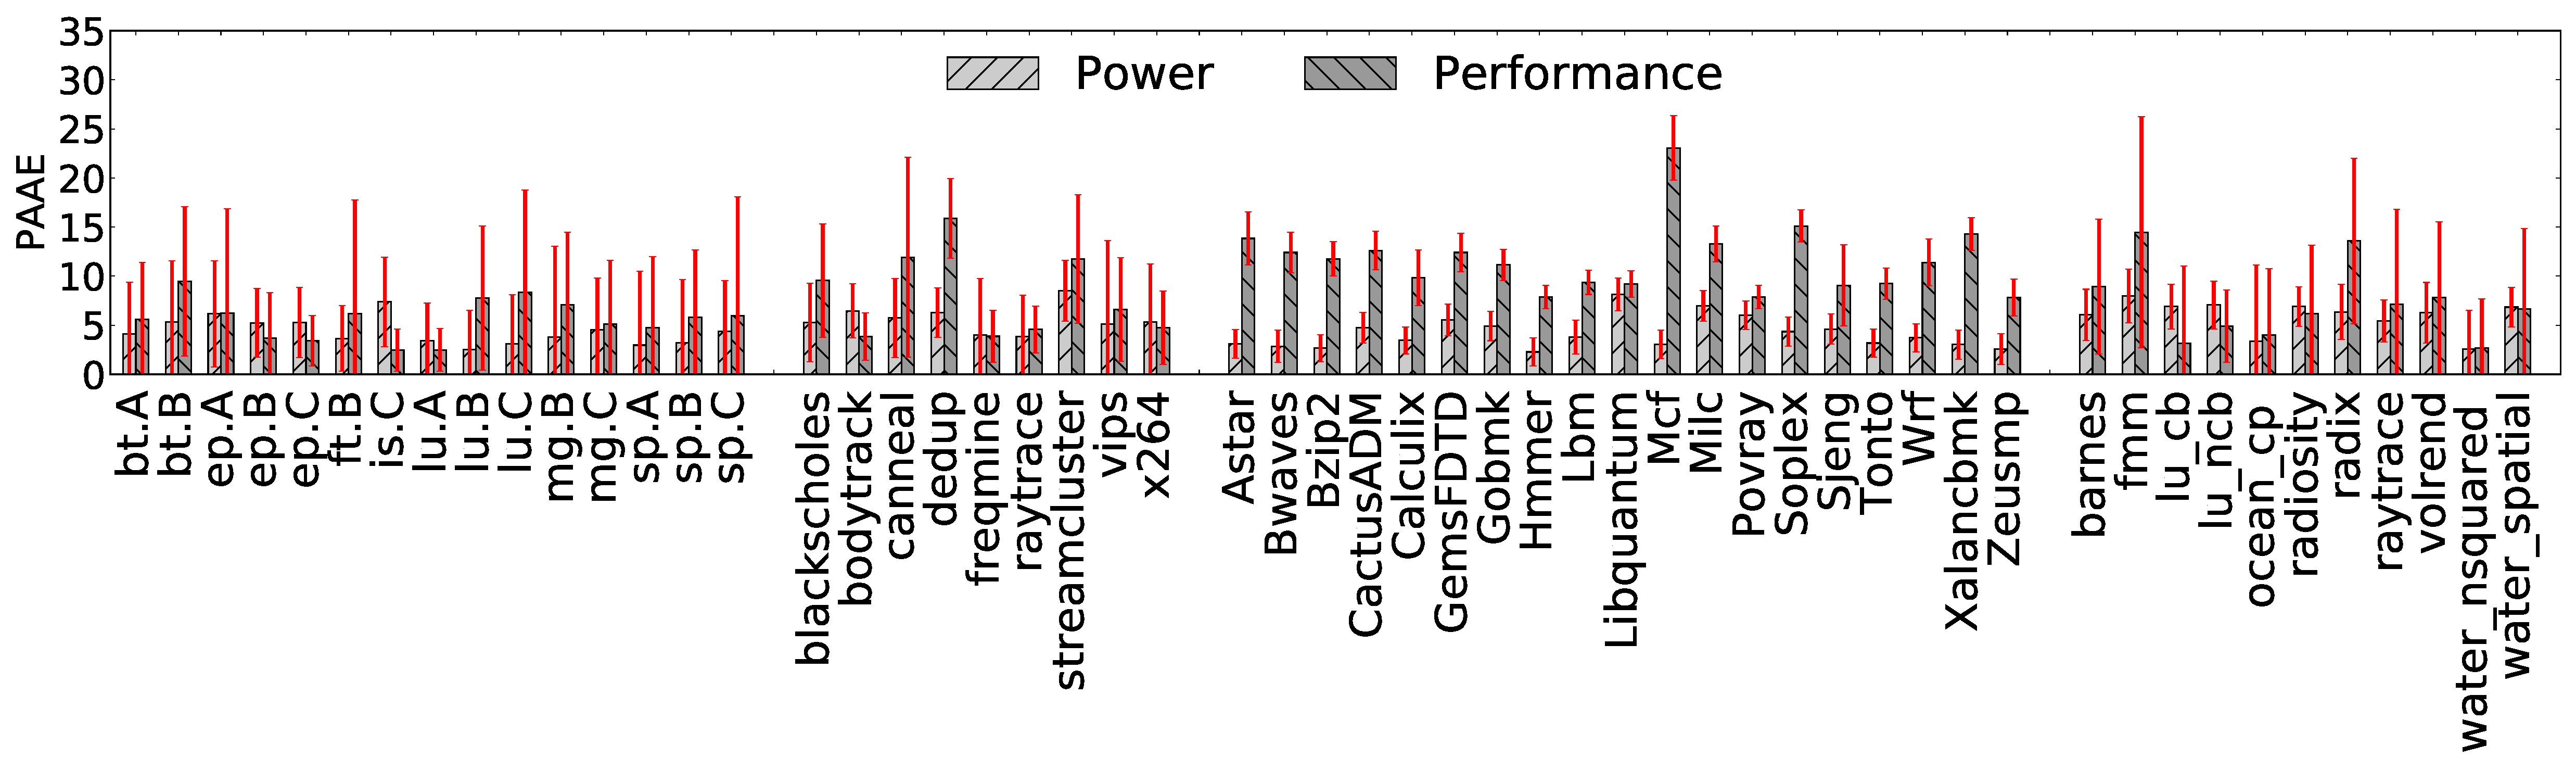
\includegraphics[width=\textwidth]{Chapter3/Figs/single-core-online/separate/intel.eps}
    %\begin{overpic}[width=\textwidth]{Chapter3/Figs/single-core-online/separate/intel.eps}
    %    \put(100,95) {TEST}
    %\end{overpic}
    \stackinset{c}{}{b}{-10pt}{\hspace{0.7cm} NAS \hspace{1cm}   PARSEC \hspace{2cm} SPEC \hspace{2cm} SPLASH}{%
    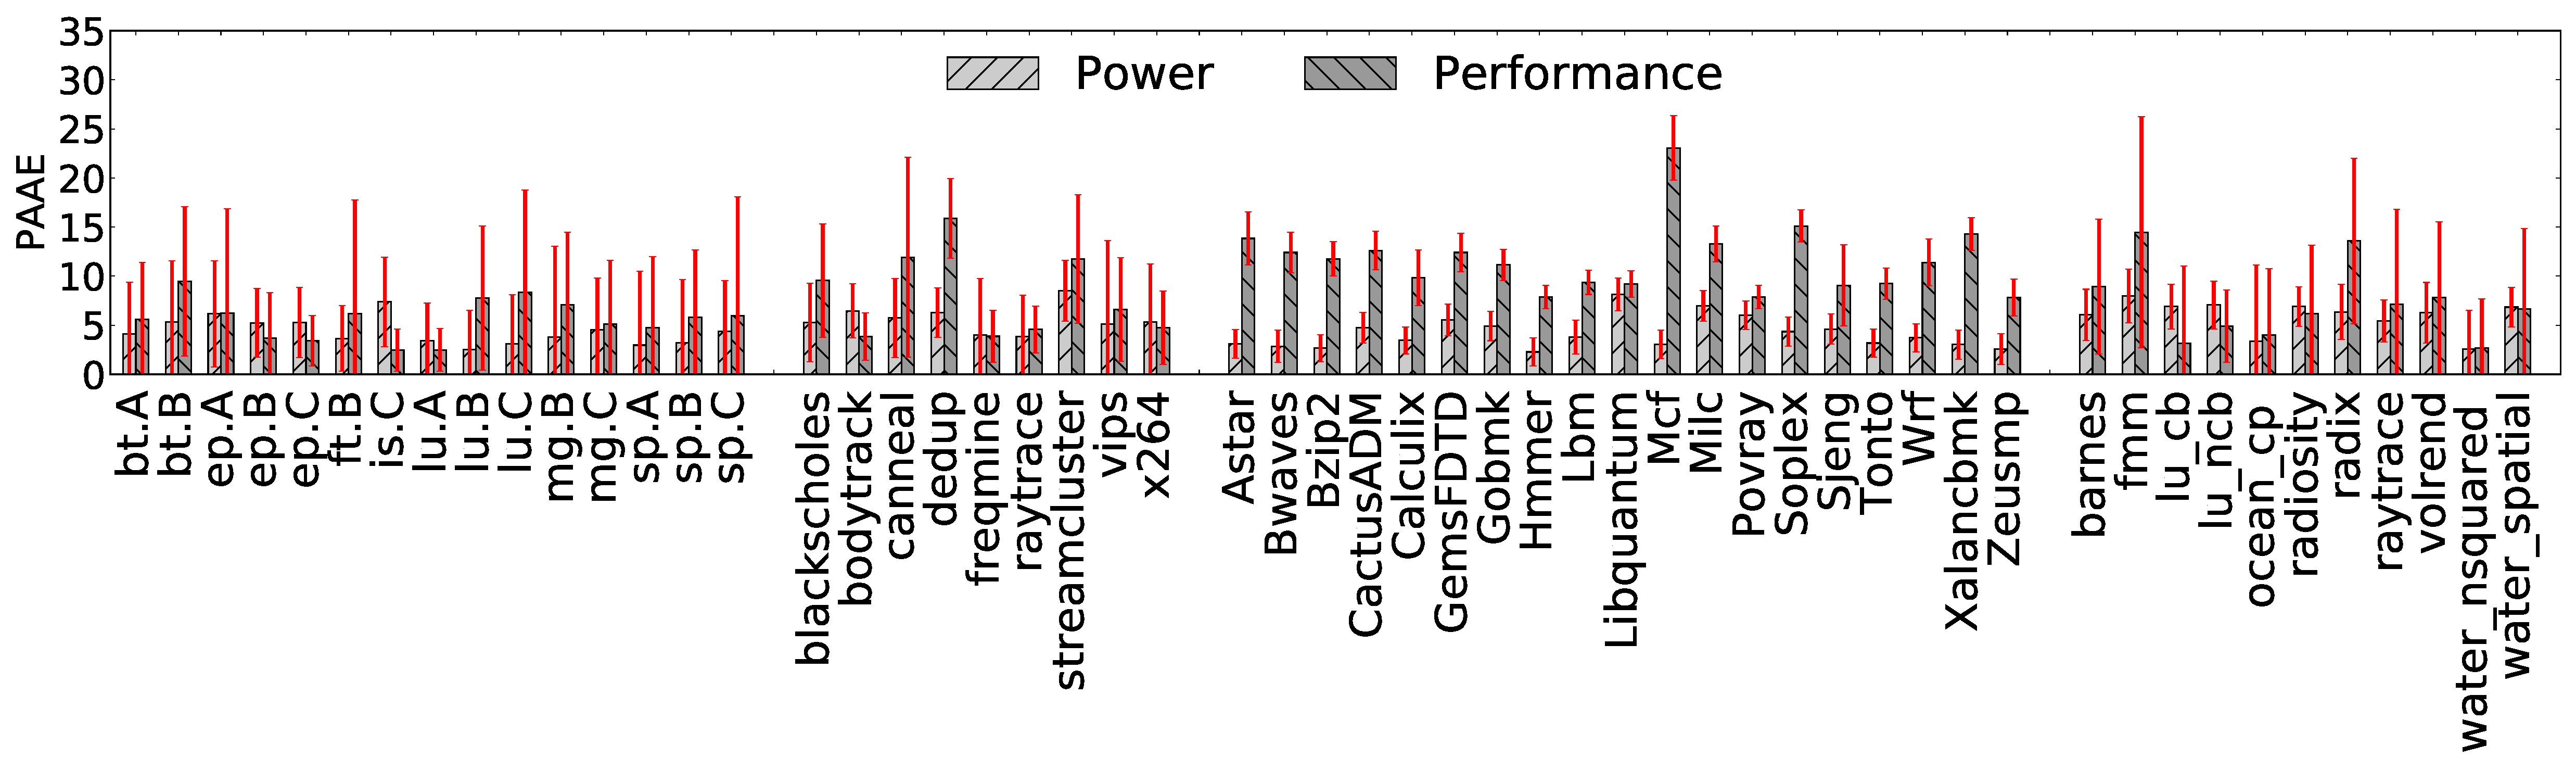
\includegraphics[width=0.95\textwidth]{Chapter3/Figs/single-core-online/separate/intel.eps}
    }    
    \caption{Intel}
    \label{fig: Intel-singlecore}
\end{subfigure}
\begin{subfigure}[t]{\textwidth}
    \centering
    \stackinset{c}{}{b}{-10pt}{\hspace{0.7cm} NAS \hspace{1cm}   PARSEC \hspace{2cm} SPEC \hspace{2cm} SPLASH}{%
    %\stackinset{c}{}{b}{-10pt}{NAS \hspace{2.3cm}   PARSEC \hspace{3cm} SPEC \hspace{2cm} SPLASH}{%
    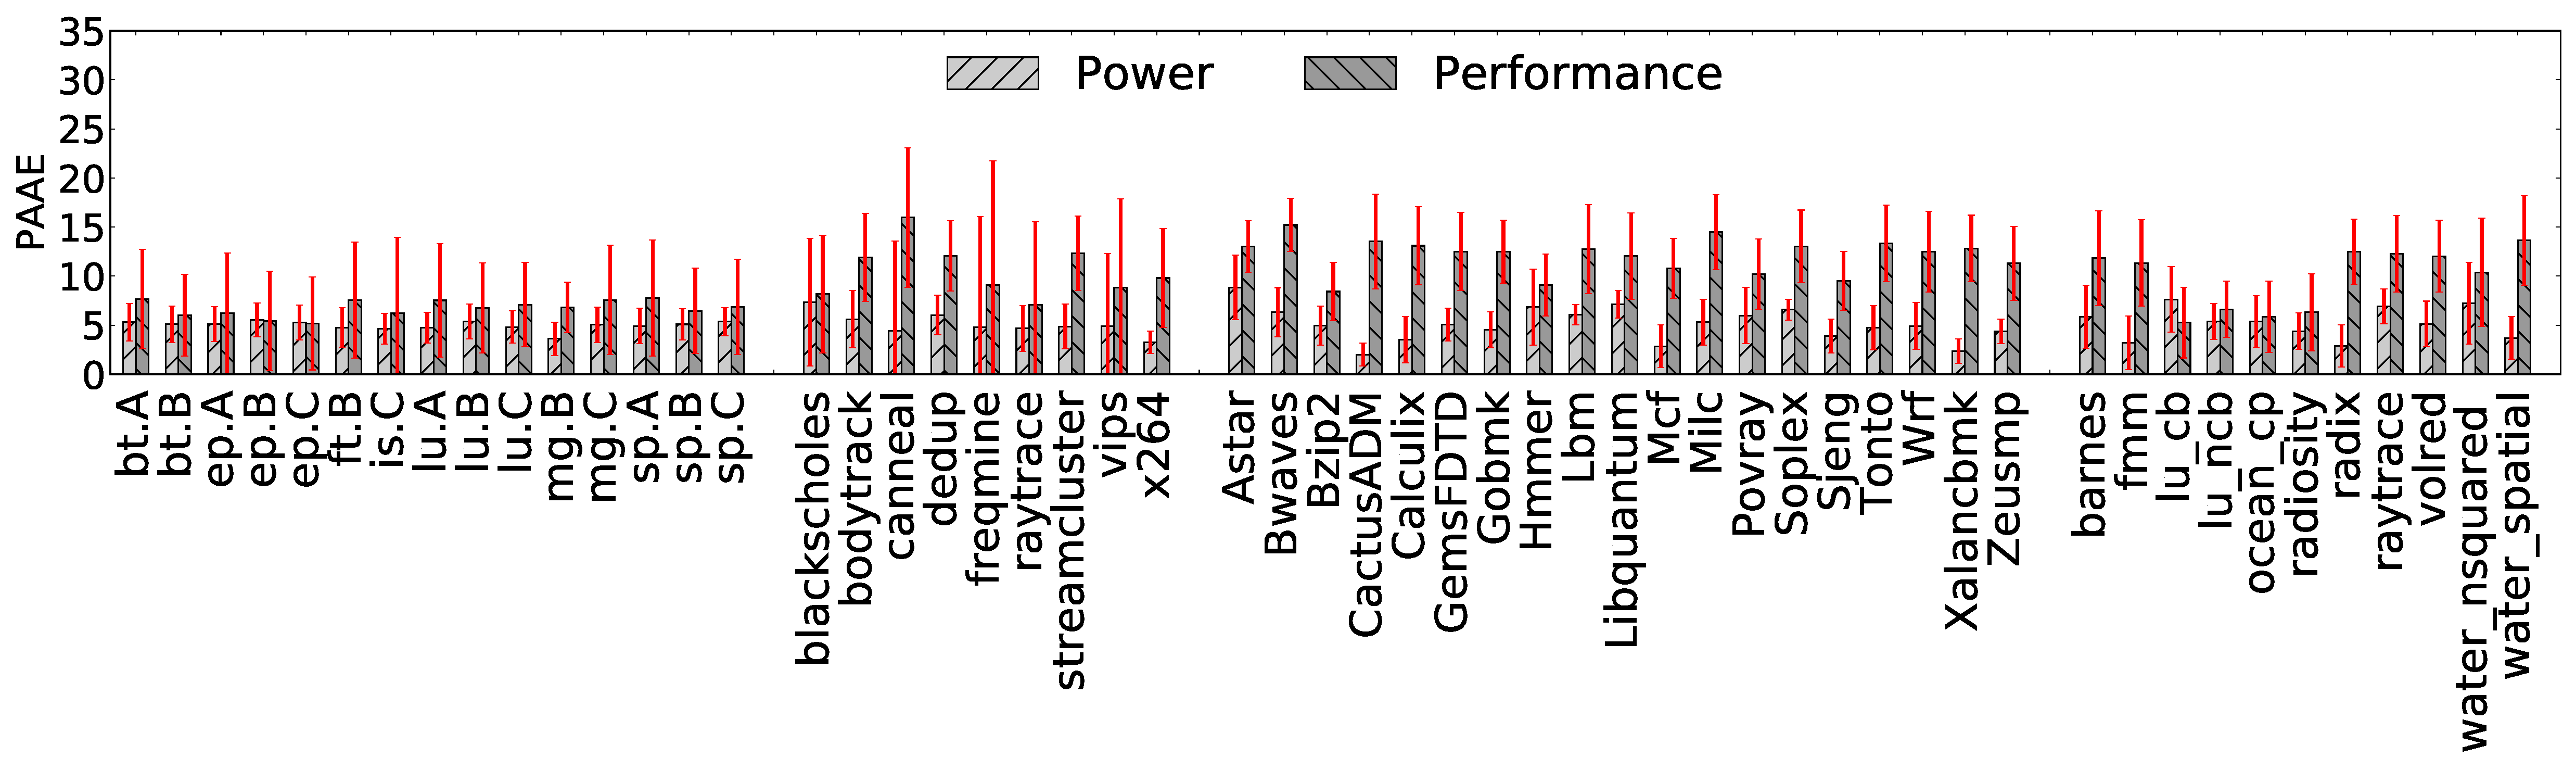
\includegraphics[width=0.95\textwidth]{Chapter3/Figs/single-core-online/separate/amd.eps}
    }    
    %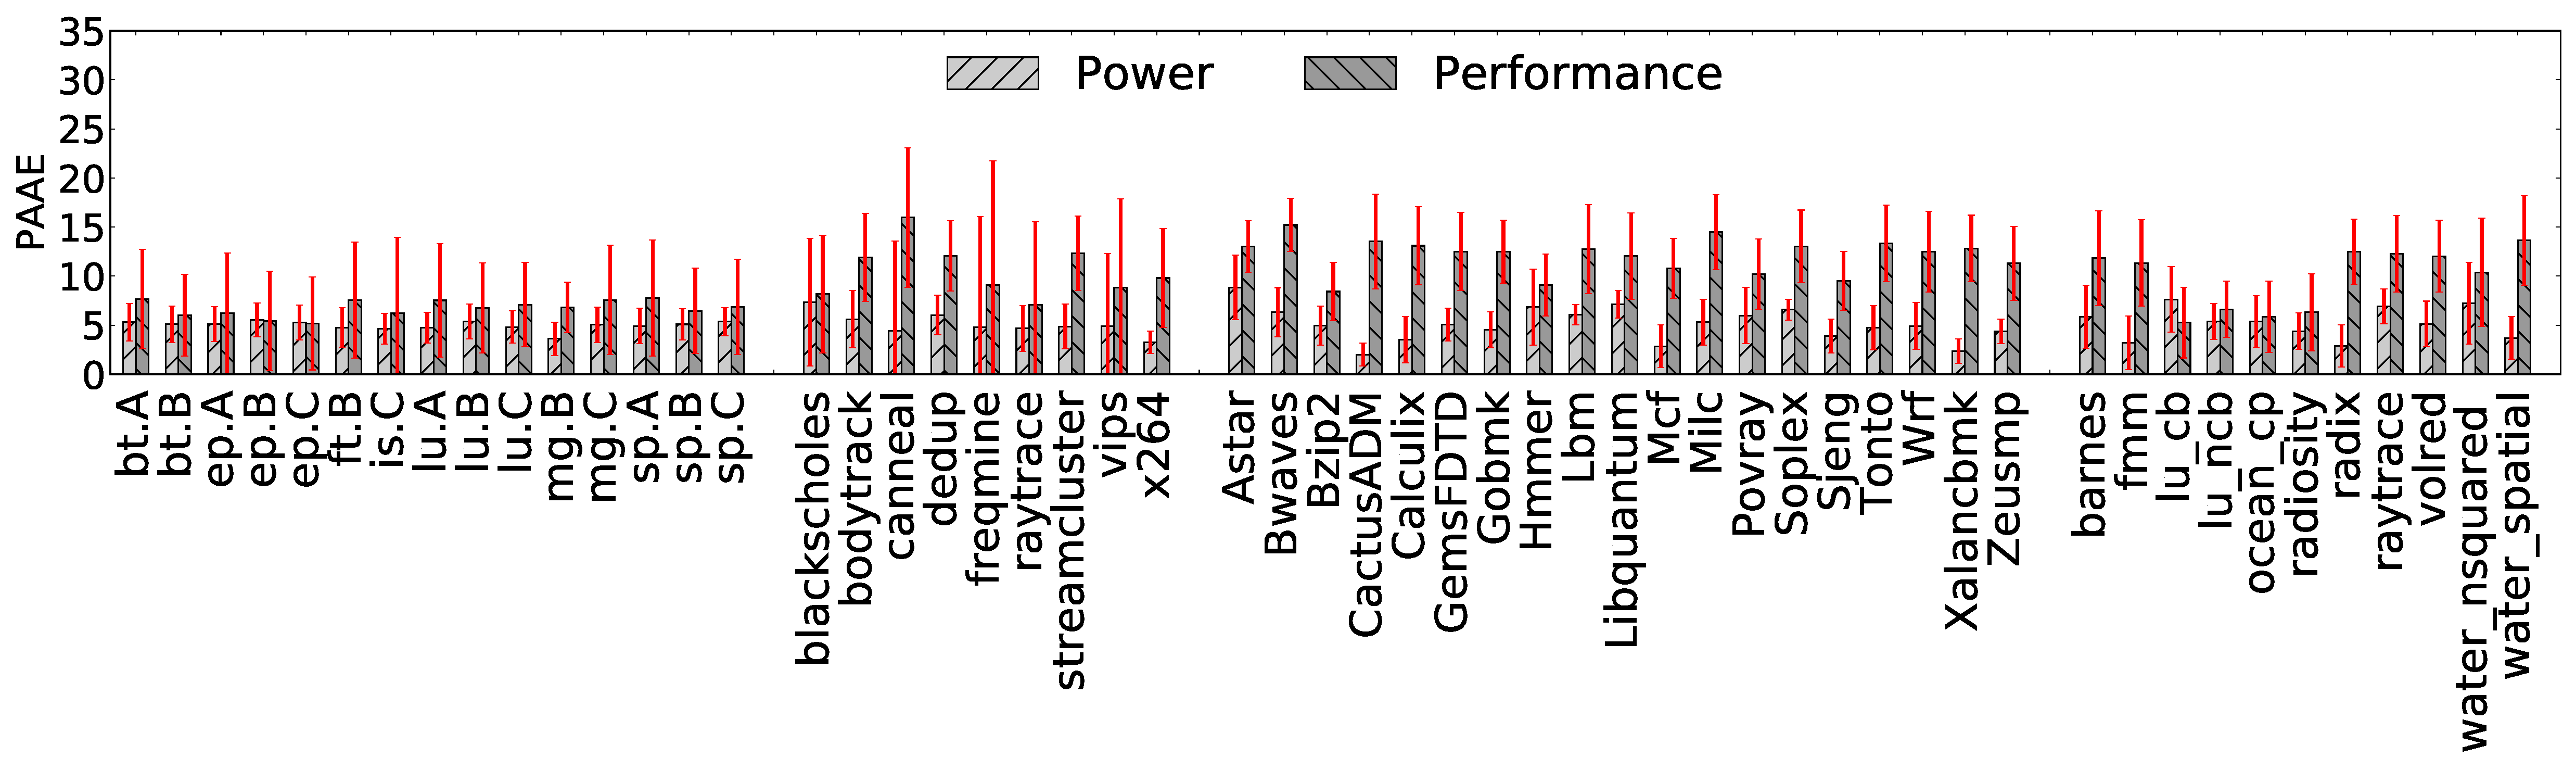
\includegraphics[width=\textwidth]{Chapter3/Figs/single-core-online/separate/amd.eps}
    \caption{AMD}
    \label{fig: amd-singlecore}
\end{subfigure}
\begin{subfigure}[t]{\textwidth}
    \centering
    %\stackinset{c}{}{b}{-10pt}{NAS \hspace{4.0cm}   PARSEC \hspace{4.5cm} SPLASH}{%
    \stackinset{c}{}{b}{-10pt}{\hspace{0.7cm} NAS \hspace{1cm}   PARSEC \hspace{5.5cm} SPLASH}{%
    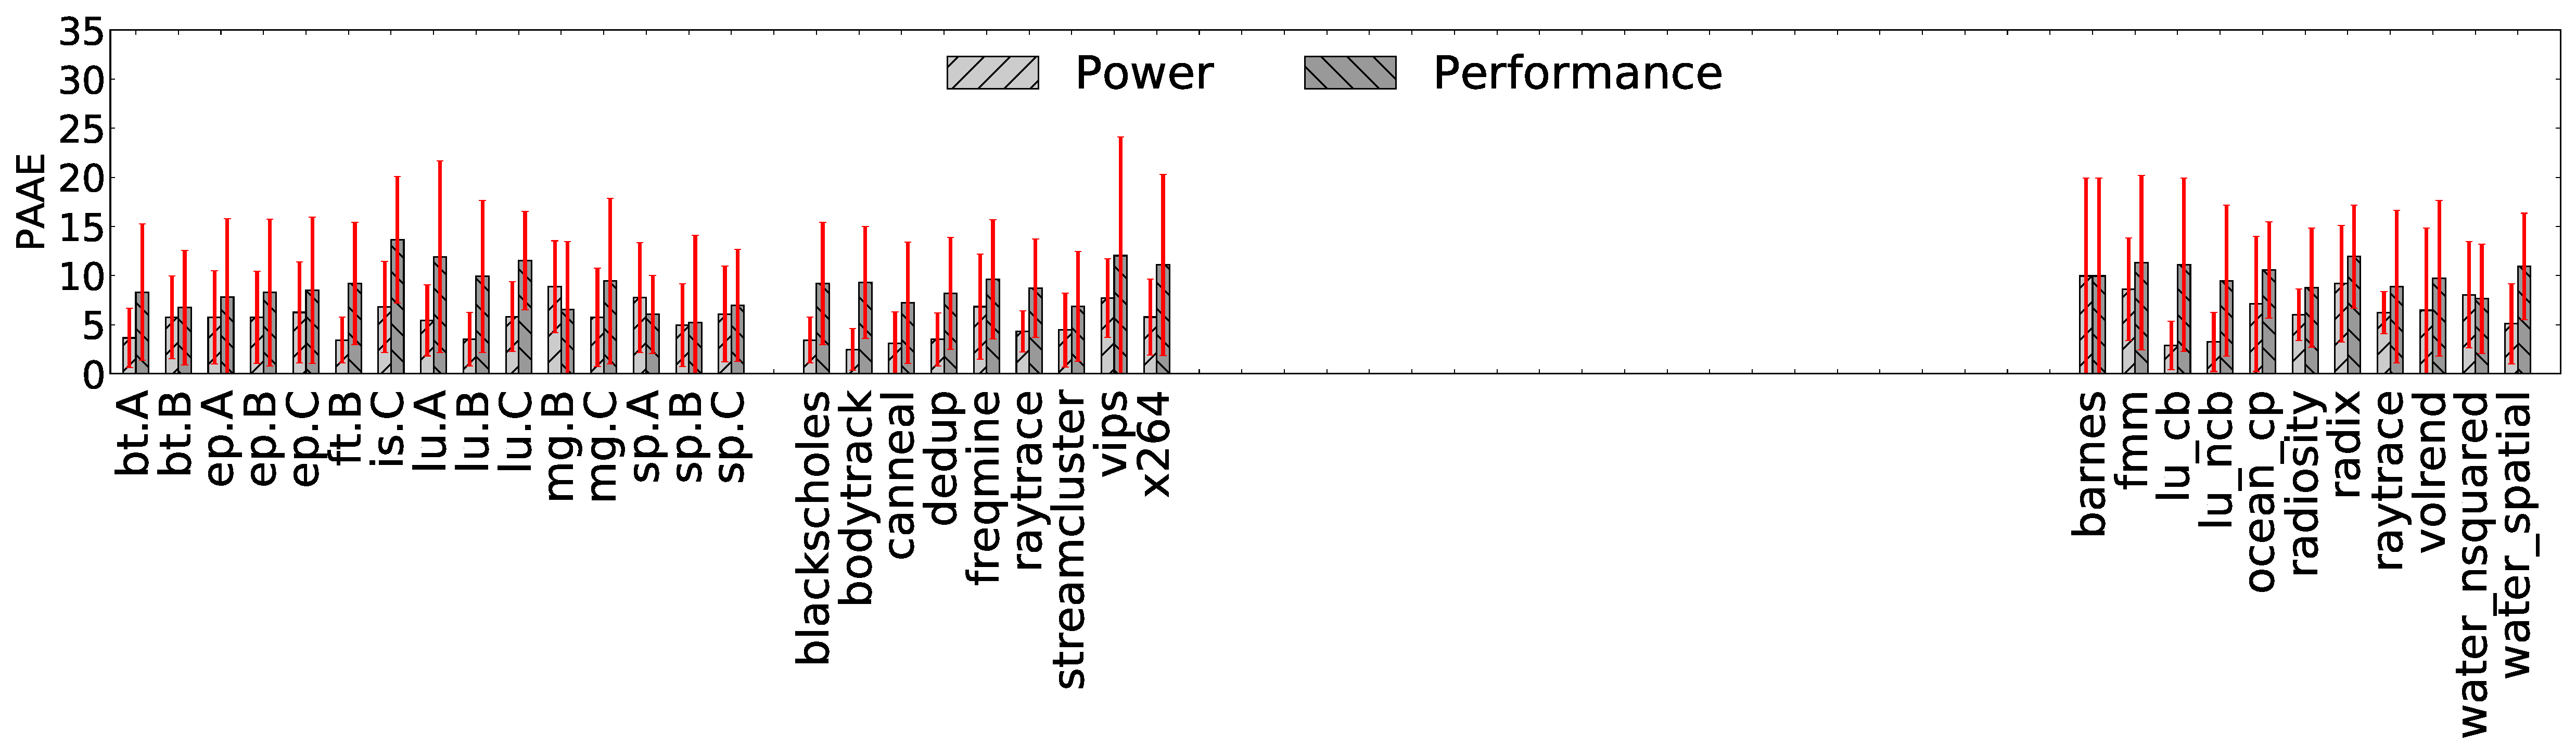
\includegraphics[width=0.95\textwidth]{Chapter3/Figs/single-core-online/separate/arm.eps}
        }
    \caption{ARM}
    \label{fig: arm-singlecore}
\end{subfigure}
    \caption[Average PAAE when predicting performance and power per benchmark on a single-core]{\captitle{Average PAAE when predicting performance and power per benchmark on a single-core.} Average PAAE when predicting performance and power on a single-core for each benchmark from four benchmark  suites across a combination of DVFS states, Cl-States and architectures. The error bars represent the STDEV. Results are shown for Intel (top), AMD (middle), and ARM (bottom). The benchmarks are organised as follows from left-to-right: NAS, PARSEC, SPEC, and SPLASH2x}.
    \label{fig: singlecoredetail} 

\end{figure} 



\section{Multicore Model Evaluation}
\label{subsection: evaluation repp-h}

The multicore evaluation of REPP is carried out in three parts. At first, we validate the
error introduced by the single-core models on multicore architectures, that is, without
considering shared resource contention (Equation~\ref{eq: critical error} and
Section~\ref{subsubsection: no-contention}).  Thereafter, we introduce the model for
shared resource contention and validate REPP without any performance or power constraint
(Section~\ref{subsubsection: technical approach}).  Finally, we validate REPP (with the
contention model) by limiting the power usage or delivering a minimum performance for a
wide spectrum of workloads on three different architectures (Section~\ref{subsubsection:
multicore evaluation with constraints}). The multiprogrammed workloads in all three cases
are generated based on the methodology described in section~\ref{subsection: batch
workloads}.  Irrespective of the how REPP is evaluated, the algorithm is invoked every
\SI{250}{\milli\second} and each experiment was run multiple times. The standard deviation
over multiple runs for each workload was low ($<$ \SI{2}{\percent}).

\looseness -1 In the first two parts (sections~\ref{subsubsection: no-contention}
and~\ref{subsubsection: technical approach}), we validate REPP by switching across all
combinations of DVFS states and Cl-States only on Intel processor.  Since the total number
of DVFS state and Cl-State combinations are 41 billion (450 per core and 4 cores).  It is
infeasible to validate for the entire spectrum.  Therefore we generate 1000 random tuples
of DVFS state, Cl-State combinations per core within the minimum and maximum DVFS state
and Cl-State ranges.  These random combinations are fixed across workloads. The
randomisation was done using the \textsf{rand()} function.  Moreover, the multiprogrammed
workloads generated are taken from SPEC CPU 2006 and PARSEC 3.0 benchmark suites. 

\looseness -1 In the third part (section~\ref{subsubsection: multicore evaluation with
constraints}), we validate REPP on three different architectures with multiprogrammed
workloads built from SPEC CPU 2006, PARSEC 3.0, NAS, and SPLASH2x.  The process of
delivering a minimum performance or limiting the power usage of the workload is done by
selecting a configuration from the predicted values that satisfy the configuration. 

The \textit{training workloads} selected for building the contention model (refer section
\ref{subsec: mult model}) in our case study are \textbf{SSSS}, \textbf{NNNN},
\textbf{TTTT}, and \textbf{FFFF} as they have a huge variation in memory footprint and CPU
requirements. 


\subsection{Multicore Models ignoring Contention} 
\label{subsubsection: no-contention}

\begin{figure}[tb!]
   \centering
    \includegraphics[width=\textwidth]{Chapter3/Figs/no-contention/without-contention-paae.eps}
    \caption[PAAE ignoring contention for shared resources]{\captitle{PAAE ignoring contention for shared resources.} PAAE when predicting \textbf{power} and \textbf{performance} across 1000 combinations of DVFS states and Cl-States per core in multicore architectures for training workloads.} 
    \label{fig: power perf prediction multicore paae}
\end{figure}


Figure~\ref{fig: power perf prediction multicore paae} shows PAAE in predicting power and
performance across 1000 combinations of DVFS states and Cl-States per core in multicore
architecture. We highlight two key points from this graph. First, observe that workloads
\textbf{SSSS} (a memory intensive workload) and \textbf{NNNN} (a compute intensive
workload) have the highest PAAE when predicting performance and power, respectively, this
is because the activity is predominant in the memory subsystem and processor,
respectively. Second, observe that the error in predicting power increases as the compute
intensiveness of the workloads increases, this is because the single-core models aggregate
the results obtained from each core and do not account for the contention due to shared
resources, thereby the compute intensive workloads which have lower activity in memory
subsystem -- compared to memory intensive workloads -- are accounted for higher activity.
Whereas the error when predicting performance increases as the memory boundedness of the
workloads increase, this can be attributed to the fact that the activity generated per
cycle in the components decreases, thereof the performance per thread. The PAAE and
Absolute Average Error (AAE) when predicting power and performance across the training
workloads are \SI{20.93}{\percent} (\SI{430}{\milli\watt}) and \SI{23.8}{\percent} (3316
MIPS).

\nomenclature[z-AAE]{AAE}{Absolute Average Error}



%start from subsubsections...
\subsection{Multicore Models including Contention without Constraints}
\label{subsubsection: technical approach}

\begin{figure}[b!]
    \centering
    \includegraphics[width=\textwidth]{Chapter3/Figs/technical/SSSN-xal-xal-astar-blackscholes-new.eps}
    \caption[Power and performance prediction for workload SSSN]{\captitle{Power and performance prediction for workload SSSN.} Runtime power and performance prediction over time (in seconds) for workload SSSN. The legend at the top is for the first two graphs, and at the bottom is for the last two graphs.}
    %\caption{Runtime power and performance prediction over time (in seconds) for workload SSSN.}
    \label{fig: power realtimeSSSN}
    %./2016/repp-extention/perf-graphs.py script to regenerate plot
\end{figure}

Figure~\ref{fig: power realtimeSSSN} shows an example of the power and performance
prediction in runtime implemented on our system for the first 20 seconds of execution for
the workload, SSSN. Specifically the workload SSSN consists of benchmarks \emph{milc},
\emph{milc}, \emph{xalancbmk} and \emph{blackscholes}. From top-to-bottom, the first (and
second) graph represents the power (and performance) as measured using RAPL (and PMC) and
the prediction made using REPP. The third and fourth graphs show the random combination
of DVFS states and Cl-States generated for individual cores, respectively, for the first 20
seconds. We highlight two results. First, REPP does show the capability to adapt to
workloads consisting of multiple thread phases (SPEC CPU 2006 and PARSEC 3.0 benchmarks
have both memory and computational bound phases).  For instance, observe at second 12,
REPP makes a \SI{11}{\milli\watt} error in predicting power, this is because of the huge
changes in DVFS states and Cl-States. In this scenario, the DVFS states for core zero, one, two,
three change from \SI{0.8}{\giga\hertz} to \SI{2.4}{\giga\hertz}, \SI{0.8}{\giga\hertz} to
\SI{2.2}{\giga\hertz}, \SI{0.8}{\giga\hertz} to \SI{2.2}{\giga\hertz} and
\SI{1.2}{\giga\hertz} to \SI{0.8}{\giga\hertz} respectively and the Cl-States change from
10 to 23, 1 to 31, 41 to 48 and 3 to 35. Observe that these errors only occur with huge
changes in DVFS states and Cl-States in rapid intervals (for example, second four).  Ozlem
\etal~\citep{Bilgir_exploringthe} on the other hand, show that rapid changes in power or
performance are seldom required in data centre environments. Second, REPP can predict
power and performance per thread, which can not be accomplished using the in-built RAPL
register. In this particular workload, we make an error of \SI{9.4}{\percent}
(\SI{384}{\milli\joule}) and 15.2\% (1500 MIPS) when predicting power and performance over
300 seconds, respectively. 

\begin{figure}[t]
   \centering
    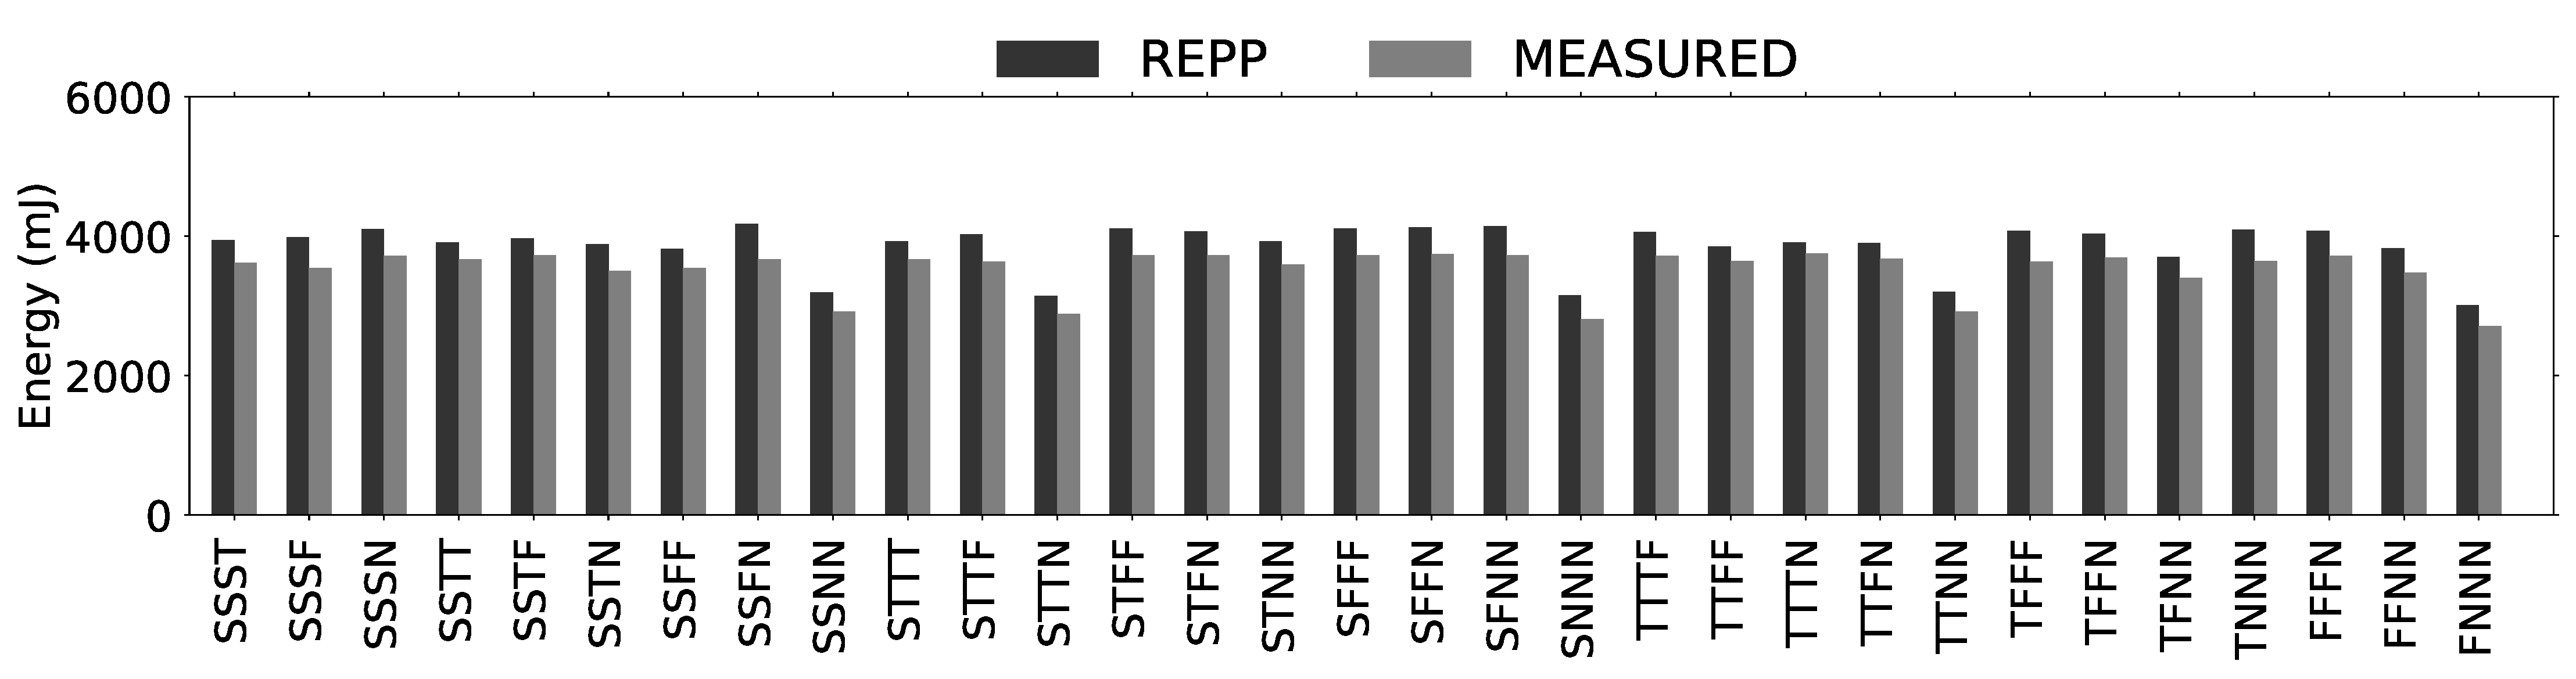
\includegraphics[width=\textwidth]{Chapter3/Figs/technical/power-paae.eps}
    \caption[Power prediction with multiple workloads without constraints]{\captitle{Power prediction for multiprogrammed workloads without constraints.} \textit{Energy consumed (\si{\milli\joule})} across all workloads on Intel processor. The $y$-axis is read as predicted (REPP) and measured (using RAPL).}
    \label{fig: power workloadswithout}
\end{figure}

Figure~\ref{fig: power workloadswithout} shows the energy consumption in
millijoules~(\SI{}{\milli\joule}) using our prediction technique, REPP and the power
measured using native RAPL register for all workloads over a period of 300 seconds when
switching across 1000 combinations of DVFS states and Cl-States. On average, workloads incur
an error in prediction of \SI{8.6}{\percent} or \SI{332.31}{\milli\joule}. Observe that
the maximum error we incur is \SI{12.1}{\percent} (\SI{507.36}{\milli\joule}) in workload
SSFN. 


\begin{figure}[t]
    \centering
    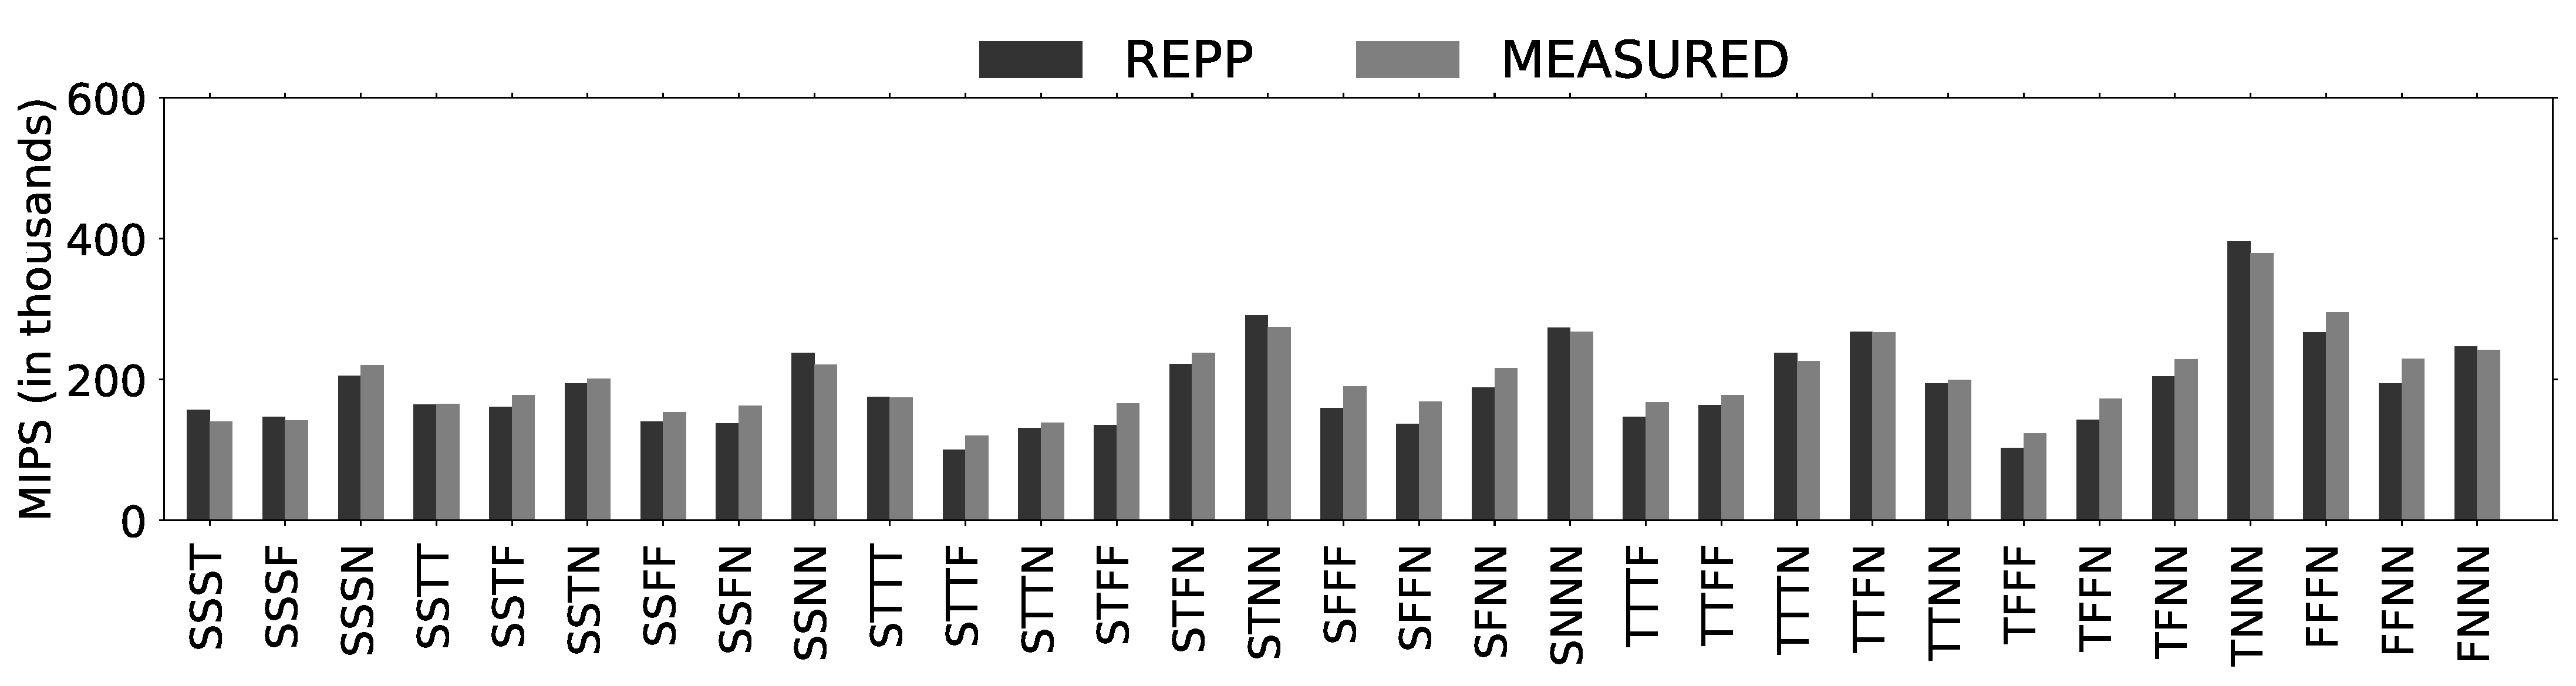
\includegraphics[width=\textwidth]{Chapter3/Figs/technical/perf-paae.eps}
    \caption[Performance prediction with multiple workloads without constraints.]{\captitle{Performance prediction for multiprogrammed workloads without constraints.} \textit{Total performance (in thousands)} across all workloads on Intel processor. The $y$-axis is read as predicted (REPP) and measured (using PMCs).}
    \label{fig: perf workloadswithout}
\end{figure}

Figure~\ref{fig: perf workloadswithout} shows the total performance (MIPS) in thousands
using our predicting technique (REPP), and the performance \texttt{measured} using PMCs
for all workloads over a period of 300 seconds when switching across 1000 combinations of
DVFS states and Cl-States. The average error we incur is \SI{8.8}{\percent} (over the 1000
combinations on all cores) and the maximum error is \SI{18.8}{\percent} in workload SFFN. 

\begin{table}[tb]
\centering
    \caption[Prediction error without constraints while disregarding certain benchmark categories]{\captitle{Performance and power prediction error without constraints while disregarding certain benchmark categories.} Error is shown in terms of PAAE.}
\scalebox{1}{    
\begin{tabular}{llccr} 
\toprule
    Label & Benchmark category & Power & Performance \\
\midrule
    N & Insensitive        & \SI{8.2}{\percent} & \SI{10.2}{\percent}    \\
    F & Cache-Friendly     & \SI{8.7}{\percent} & \SI{9.8}{\percent} \\
    T & Cache-Fitting      & \SI{9.6}{\percent} & \SI{9.9}{\percent} \\
    S & Thrashing          & \SI{8.2}{\percent} & \SI{7.5}{\percent} \\

\bottomrule
\end{tabular}
}
\label{tab: ignoringbenchmark}
\end{table}

Table~\ref{tab: ignoringbenchmark} shows the power and performance prediction error
without constraints for the remaining multiprogrammed workloads when disregarding certain
benchmark categories. It is observed that the power and prediction error for the remaining
benchmarks even after disregarding a subset of benchmarks is (approximately) same. 

Figure~\ref{fig: power workloadswithout} and~\ref{fig: perf workloadswithout} demonstrate that REPP
has been validated under multiple combinations of DVFS states and Cl-States across 35
multiprogrammed workloads. Moreover, each bar in the histogram represents a summary of the
workload execution, similar to Figure~\ref{fig: power realtimeSSSN}.
 
%start from subsubsections...  
\subsection{Multicore Models including Contention with Constraints}

\label{subsubsection: multicore evaluation with constraints}

In this section, we validate multicore models of REPP by predicting performance and power
at the hardware settings DVFS states and Cl-States (Section~\ref{subsec: algo}), and then
select a configuration to satisfy the user provided constraint.  This constraint is
defined as either delivering a minimum performance, or not violating a power target.
Therefore, to satisfy either of these constraints, REPP provides a dynamic configuration
selector.


\subsubsection{REPP Configuration Selector}
\label{subsubsec: config selec}
\nomenclature[g-omega]{$\omega$}{The performance or power constraint per core}


\looseness -1 Modern data centres have power constraints (e.g., power capping) and run
multiple application instances with different performance constraints.  This requires an
algorithm to select a configuration per core such that the performance and power
constraints are met per core and/or per application, given by $\omega$. To ensure that
these constraints are met, REPP dynamically selects a configuration per core every
\SI{250}{\milli\second} by performing a linear search for the DVFS state that is the
nearest to the given constraint; next, REPP selects the Cl-State for the given DVFS
state that satisfies the constraint. This selected configuration, DVFS state, Cl-State, is
used to ensure that the constraint is met for each interval. 

Figure~\ref{fig: repphconfigselec} demonstrates a configuration selector to satisfy a user
defined power or performance constraint of \SI{40}{\percent}. We build one such model to
predict performance or power per core. The single-core models predict performance and
power for each configuration available in the 2-D space of DVFS state and Cl-State. We
repeat the aforementioned process for each core at the same time.


\begin{figure}
    \centering
    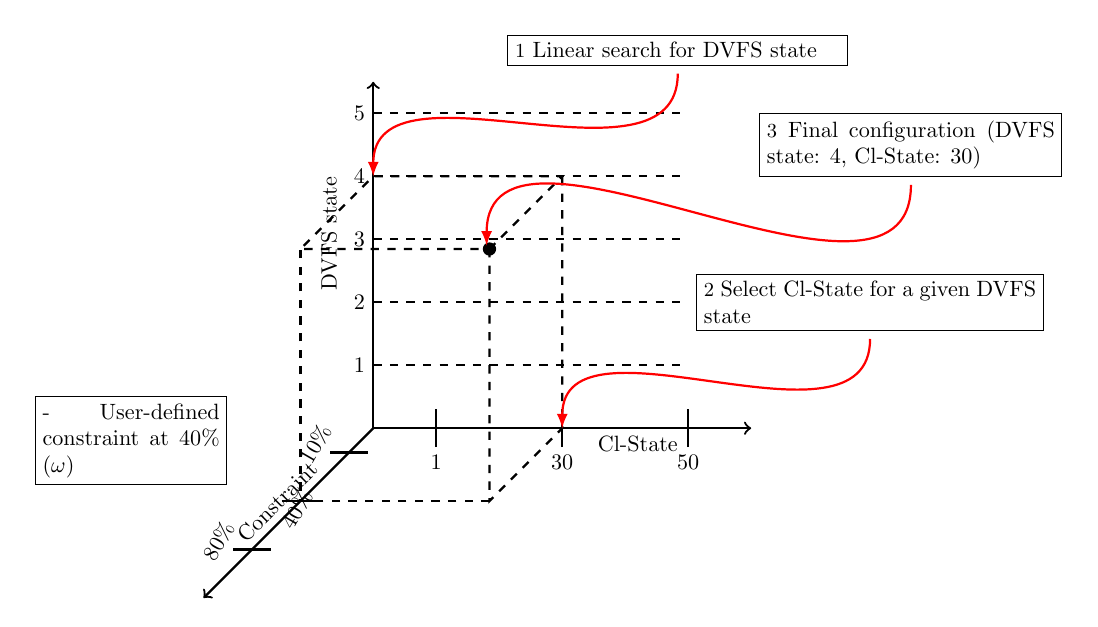
\begin{tikzpicture}[thick,scale=0.8, every node/.style={transform shape}]


    \draw[->] (0,0,0)-- node[pos=.7,below] {Cl-State} ++(6,0,0);
    \draw[->] (0,0,0)--++(0,5.5,0) node[pos=.75, left=7mm,rotate=90]{DVFS state};% ++(0,0,0);
    \draw[->] (0,0,0)--++(0,0,7) node[midway, sloped, above] {Constraint};

    \draw[-] (1,-.3,0) node[below]{1}--(1,.3,0);
    \draw[-] (3,-.3,0) node[below]{30}--(3,.3,0);
    \draw[-] (5,-.3,0) node[below]{50}--(5,.3,0);

    \draw[-] (-0.3,0,1) node[above, rotate=60]{10\%}--(0.3,0,1);
    \draw[-] (-0.3,0,3) node[below, rotate=60]{40\%}--(0.3,0,3);
    \draw[-] (-0.3,0,5) node[above, rotate=60]{80\%}--(0.3,0,5);

    \fill (3,4,3) circle(3pt);

    \draw[dashed] (3,4,3)--(3,4,0)--(0,4,0)--(0,4,3)--cycle;
    \draw[dashed] (3,4,3)--(3,0,3)--(3,0,0)--(3,4,0);
    \draw[dashed] (3,0,3)--(0,0,3)--(0,4,3);


    \foreach \i in {1,2,...,5}
       \draw[dashed] (0,\i,0) node[left] {\i} --++(5,0,0);

    \node [anchor=west] (note2) at (2,6) {
        \fbox{\begin{minipage}{14.7em}
            {\small \circled{1}} Linear search for DVFS state
    \end{minipage}}};

    \node [anchor=west] (notex) at (5,2) {
        \fbox{\begin{minipage}{15em}
            {\small \circled{2}} Select Cl-State for a given DVFS state
    \end{minipage}}};

    \node [anchor=west] (notea) at (-5.5,-0.2) {
        \fbox{\begin{minipage}{8.0em}
            - User-defined constraint at 40\% ($\omega$)
    \end{minipage}}};

    \node [anchor=west] (noteaa) at (6,4.5) {
        \fbox{\begin{minipage}{13em}
            {\small \circled{3}} Final configuration (DVFS state: 4, Cl-State: 30)
    \end{minipage}}};

    \draw [-latex, thick, red] (note2) to[out=270, in=90] (0,4);
    \draw [-latex, thick, red] (notex) to[out=270, in=90] (3,0);
    \draw [-latex, thick, red] (noteaa) to[out=270, in=90] (1.8,2.9);

    \end{tikzpicture}
    \caption[REPP configuration selector]{\captitle{REPP configuration selector.} An example of the configuration selector to satisfy a user-defined constraint of \SI{40}{\percent} for either power or performance for a single-core.}
\usetikzlibrary{positioning}
\label{fig: repphconfigselec}
\end{figure}


In our study, the performance and power constraints are given at a system level. These
constraints are  distributed  homogeneously across all cores. For example, if an AMD
server can only consume \SI{600}{\watt}, that power constraint is distributed
\SI{25}{\percent} per core, allowing each core to consume \SI{150}{\watt} (it would be
\SI{50}{\percent} on ARM). In this aforementioned example, $\omega$ is \SI{150}{\watt}.
At runtime, for the spawned applications, REPP samples application behaviour
periodically and uses the models built to predict performance and power at all
configurations. REPP then selects the configuration for each interval to satisfy the
local constraint.


\subsubsection{Experiments}
\label{subsubsec: experiments repph}

We perform two types of experiments: one for validating the power capping mechanism and
the other for delivering a minimum performance. We define two input parameters: (a)
frequency of change, and (b) $\chi$, which represents load or power.  The average load
offered by the applications is constant between two load changes, which can occur every
\textbf{load\_change interval} (1, 6, or 9 seconds), based on a \textbf{change\_factor},
as follows.  Load starts at a minimum, and varies by multiplying load by change\_factor
$\tau$ until it reaches a maximum load $\chi_{\mathit{max}}$; thereafter, the load is
multiplied by the negative value of change\_factor until it reaches the minimum
$\chi_{\mathit{min}}$.

\looseness -1 The values of change\_factor tested were \SI{20}{\percent} (\textbf{Low}),
\SI{35}{\percent} (\textbf{Mid}), and \SI{50}{\percent} (\textbf{High}). The minimum load
is defined as the sum of smallest IPS for all four applications running at minimum
frequency; similarly, maximum load is the sum of highest IPS for all four applications at
maximum frequency. In another set of experiments, we change the power consumed by the
workload similar to the load offered by the workload. 

\looseness -1 Mathematically, the experiment conducted for a load\_change interval 1 can
be represented as follows: In Equation~\ref{eq: topofcurve}, $\psi$ represents the number
of datapoints before the maximum load/power ($\chi_{\mathit{max}}$), and in
Equation~\ref{eq: eachterm}, $\chi(\kappa)$ shows the datapoint $\kappa$ in the sequence.

\vspace{0.2cm}

\begin{equation}
    \label{eq: topofcurve}
    \psi = \Bigl\lfloor\dfrac{\log(\chi_{\mathit{max}}/\chi_{\mathit{min}})}{\log(1+\tau)}\Bigr\rfloor\qquad                   
\end{equation}

\vspace{0.2cm}

\begin{equation}
    \label{eq: eachterm}
    \chi(\kappa) =
\left\{
    \begin{array}{ll}
        \chi_{\mathit{min}} \times (1+\tau)^{n}  & 0 \leq n \leq \psi\\
        \chi_{\mathit{max}} \times (1+\tau)^{2\psi-n}  & \psi < n \leq 2\psi
    \end{array}
\right.                    
\end{equation} 


\vspace{0.2cm}

\nomenclature[g-psi]{$\psi$}{Number of datapoints before the peak in a step-wise monotonic function}
\nomenclature[g-tau]{$\tau$}{Change\_factor for the step-wise monotonic function}
\nomenclature[g-chi]{$\chi$}{Load (IPS) or power in a step-wise monotonic function}
\nomenclature[g-chi]{$\chi(\kappa)$}{$\kappa^{th}$ element in the data sequence for either load or power}
\nomenclature[g-chi]{$\chi(min), \chi(max)$}{The minimum, maximum value of load or power}


The error occurs when REPP selects a configuration that makes the application fall short
of the minimum required performance (or exceed the maximum power requirement) in a given
mapping interval.

We ran ten experiments for power and ten for performance.  Nine of them come from the
combinations of the two parameters (frequency of change and load/power) described above;
the tenth comes from a \textbf{Random} setting within fixed boundaries of either power or
performance. Selecting a broad spectrum of load (or power) and frequency of change allowed
us to validate REPP across multiple combination of configurations at runtime. 

\subsection*{Evaluation of the Multicore Models with Constraints}
\label{subsubsec: eval repph}

We present the results, and evaluate REPP when predicting performance and power on
multicore processors by selecting a configuration in a single step to meet power and
performance requirements for 35 multiprogrammed workloads across 20 experiments (ten for
power and ten for performance).  The prediction error is computed over a period of 400
seconds for all DVFS states and Cl-States. The error metric indicates that the constraint
was violated by that amount, which occurs when REPP selects a configuration that makes
the application fall short of the minimum required performance (or exceed the maximum
power requirement) in a given mapping interval. 

\begin{figure}[t]
   \centering
    \begin{subfigure}{\textwidth}
        \centering
        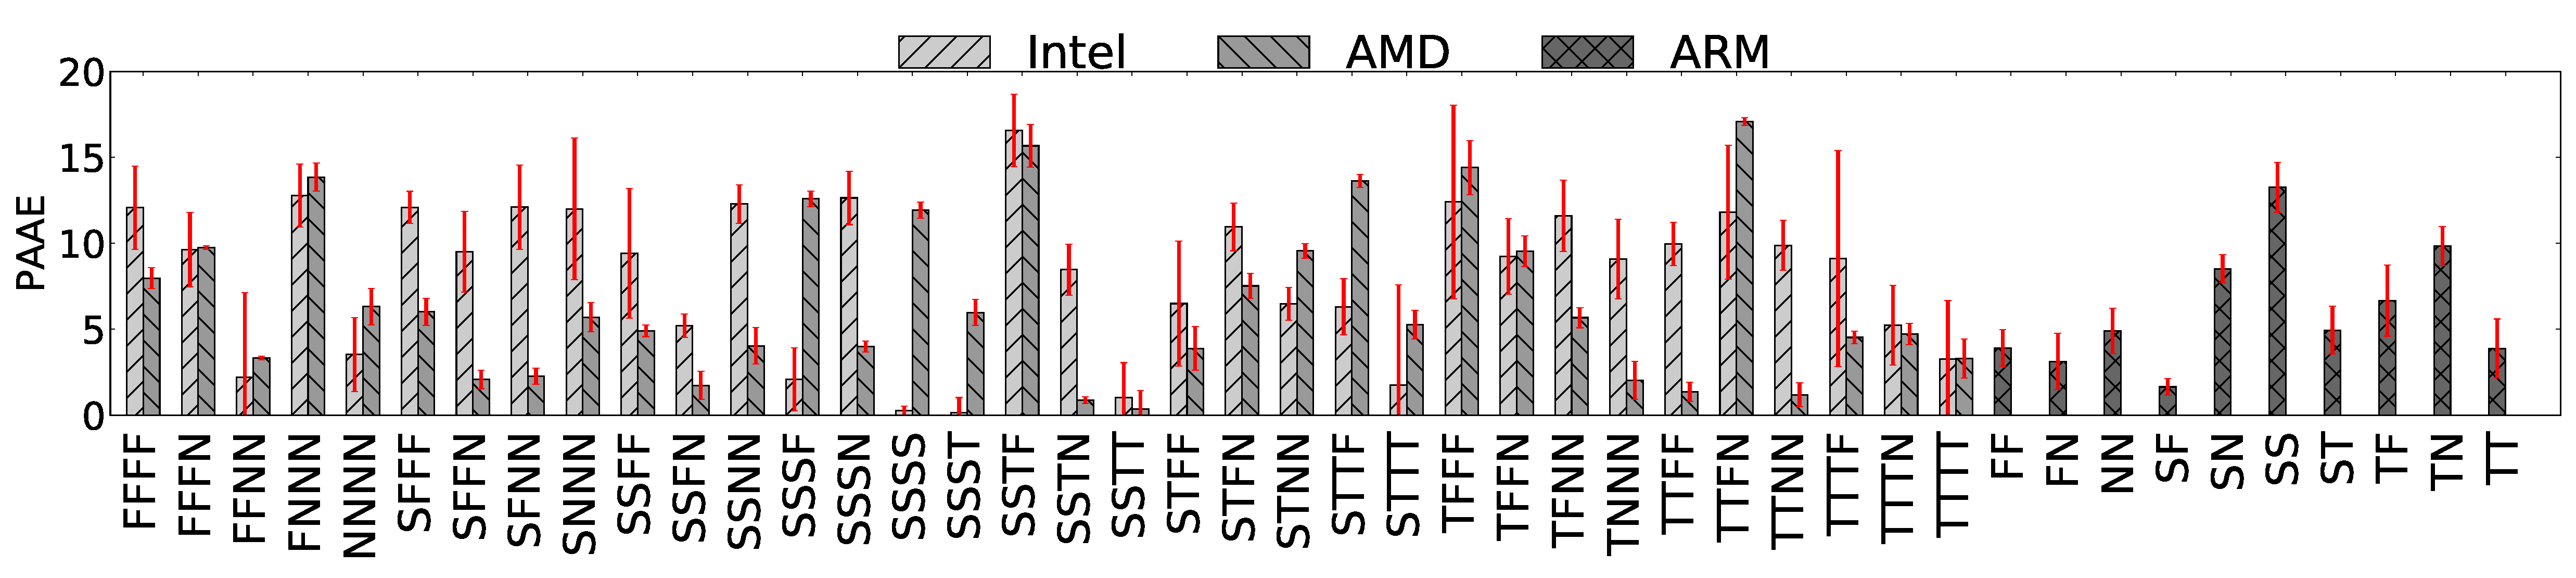
\includegraphics[width=\linewidth]{Chapter3/Figs/multicore/power-shorter-paae.eps}
        \caption{Power}
        \label{fig: power paae}
    \end{subfigure}
    \begin{subfigure}{\textwidth}
        \centering
        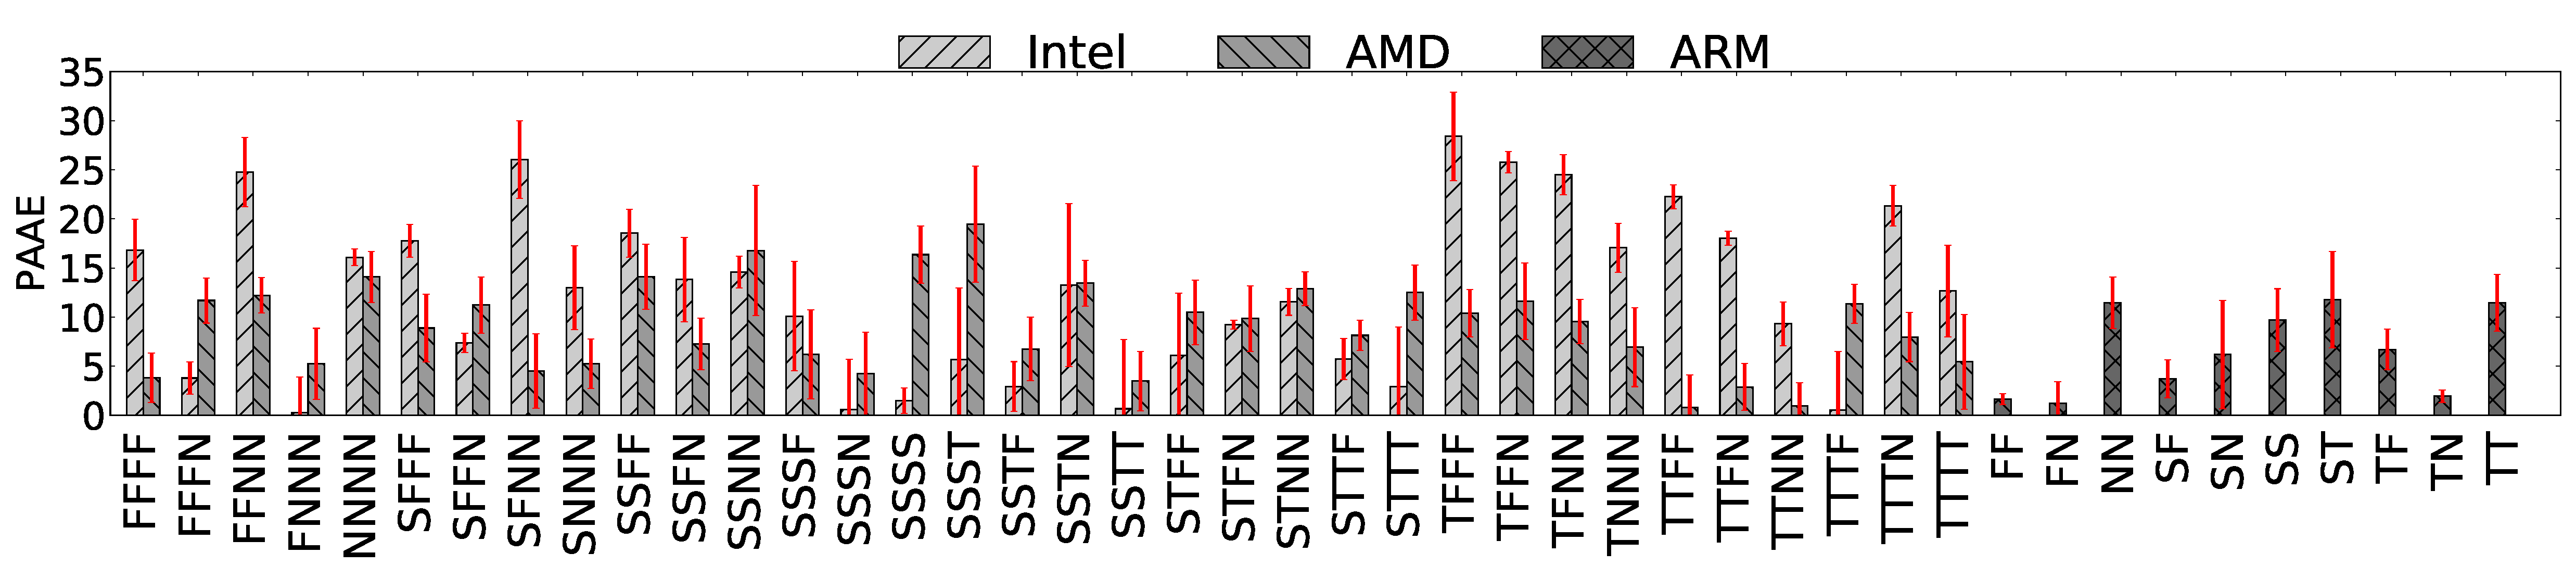
\includegraphics[width=\linewidth]{Chapter3/Figs/multicore/perf-shorter-paae.eps}
        \caption{Performance}
        \label{fig: perf paae}
    \end{subfigure} \caption[Average PAAE for REPP with multiple
    constraints]{\captitle{Average PAAE for REPP with multiple constraints.} Average
    PAAE when predicting power (\ref{fig: power paae}) and performance (\ref{fig: perf
    paae}) for all workloads under Low, Mid, High and Random change\_factors in multicore
    architectures. The error bars represent STDEV across change\_factors. The $x$-axis
    shows multiprogrammed workloads.} 
\label{fig: multicore result} 
\end{figure}

\looseness -1 Figure~\ref{fig: multicore result} shows the average PAAE for each workload when meeting
the performance (ARM \SI{7.1}{\percent}, AMD \SI{9.02}{\percent}, and Intel
\SI{7.1}{\percent}) and power (ARM \SI{6.0}{\percent}, AMD \SI{6.6}{\percent}, and Intel
\SI{8.1}{\percent}) requirements in ten experiments across architectures. The error bars
represent the STDEV across ten experiments for power and performance, which is less than
\SI{5.3}{\percent} for each workload. We focus on analysing those workloads with an error
greater than \SI{10}{\percent} in both architectures. When predicting power, we observe an
error of \SI{13.8}{\percent} (\SI{654.86}{\milli\joule}) on AMD for workload \texttt{FNNN}
that contains \emph{ep.C}, which has very high activity ratio in BPU (4.2542) and FE
(13.752).  Similarly for workload \texttt{TTFN}, Intel has a higher error
\SI{11.8}{\percent} (\SI{11.34}{\milli\joule}) than AMD, because on Intel we run two
instances of \emph{radix}, whereas on AMD we run a single one. Recall that the
multiprogrammed are generated based on the methodology described in
Section~\ref{subsection: batch workloads}, therefore we can not control  the number of
instances in a given workload. When predicting performance, we observe an error of 26.0\%
for \texttt{SFNN} on Intel because we run \emph{lu\_ncb}, which has non contiguous blocks
of memory and the activity ratio in LLC is higher relative to other benchmarks.
Similarly, workloads \texttt{TTTF} on AMD and \texttt{TTFN} on Intel have a power
prediction error of \SI{11.3}{\percent} and \SI{18.0}{\percent}, respectively, because
\emph{radix} is part of the multiprogrammed workloads.  The maximum performance error on
AMD, ARM and Intel are 19.4\% (769 MIPS for \texttt{SSST}), \SI{11.7}{\percent} (5389 MIPS
for \texttt{ST}) and \SI{28.4}{\percent} (13611 MIPS for \texttt{TFFF}). Similarly the
maximum power error AMD, ARM and Intel are \SI{17.0}{\percent} (\SI{101.72}{\milli\joule}
for \texttt{TTFN}), \SI{13.3}{\percent} (\SI{10}{\milli\joule} for \texttt{SS}) and
\SI{16.6}{\percent} (\SI{37.24}{\milli\joule} for \texttt{SSTF}), respectively. 

\begin{figure*}[tb!]
   \centering
    \begin{subfigure}{0.32\textwidth}
        \centering
        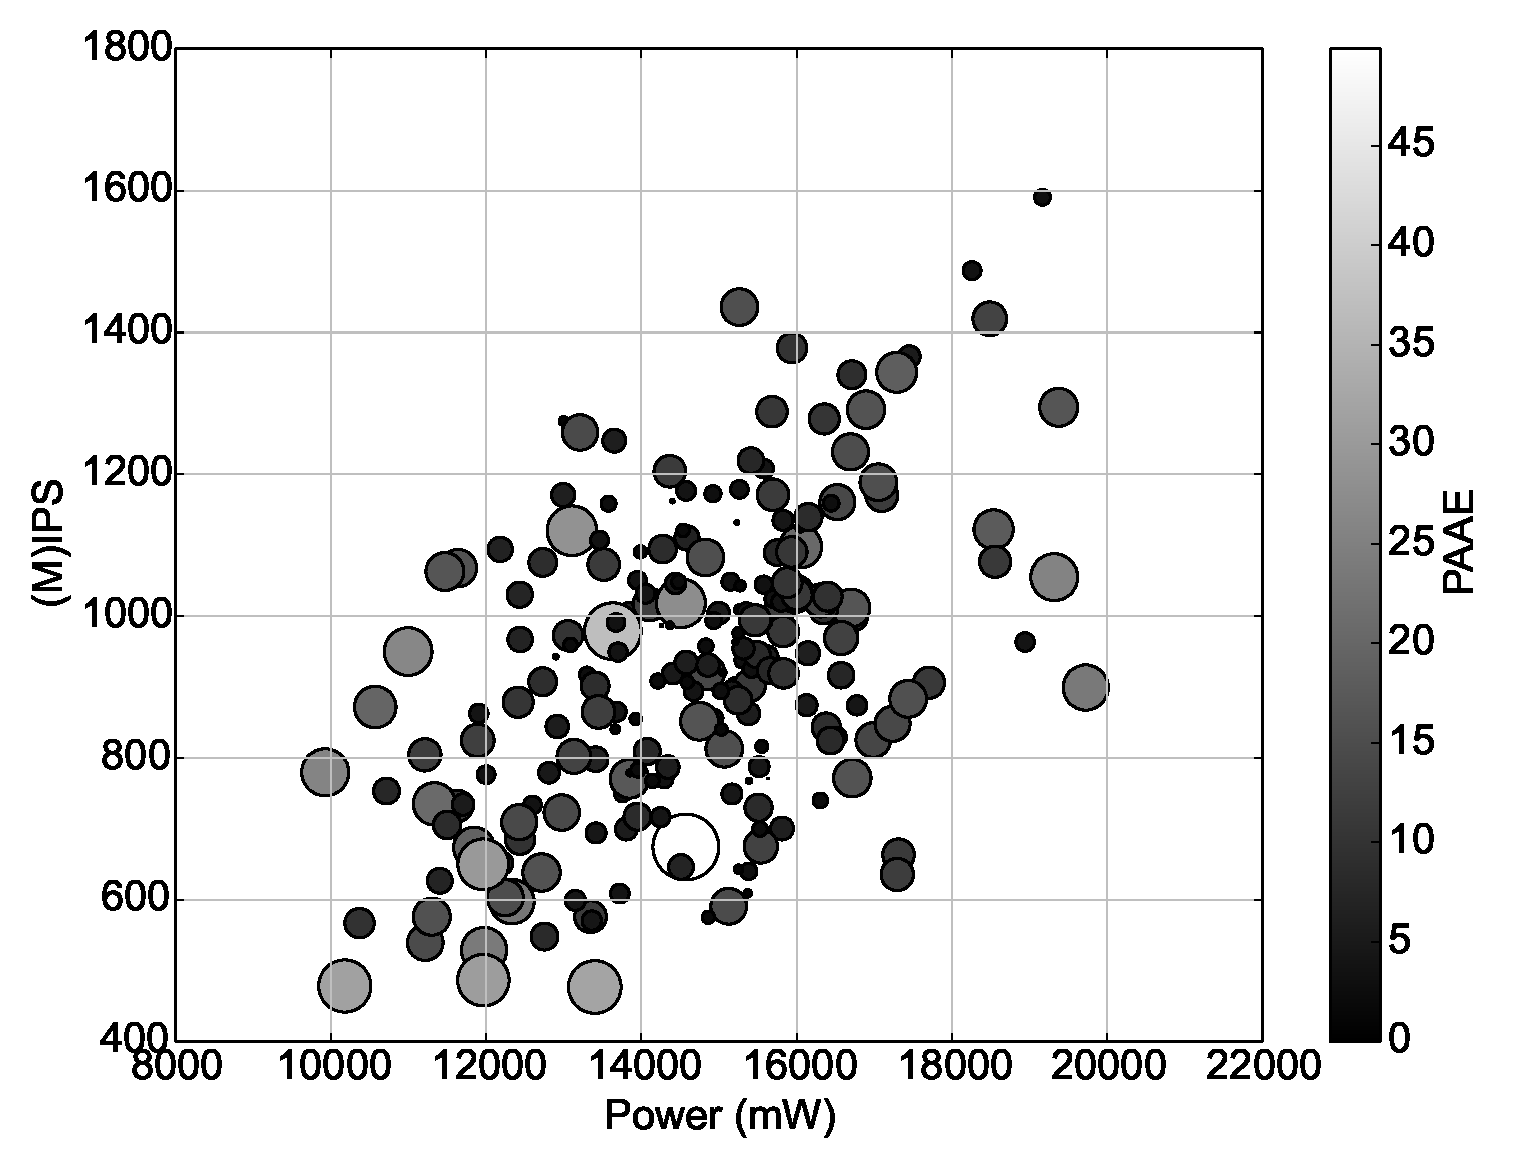
\includegraphics[width=\textwidth]{Chapter3/Figs/scatter/SSTN.eps}
        \caption{SSTN}
        \label{fig: SSTN}
    \end{subfigure}
    \begin{subfigure}{.32\textwidth}
        \centering
        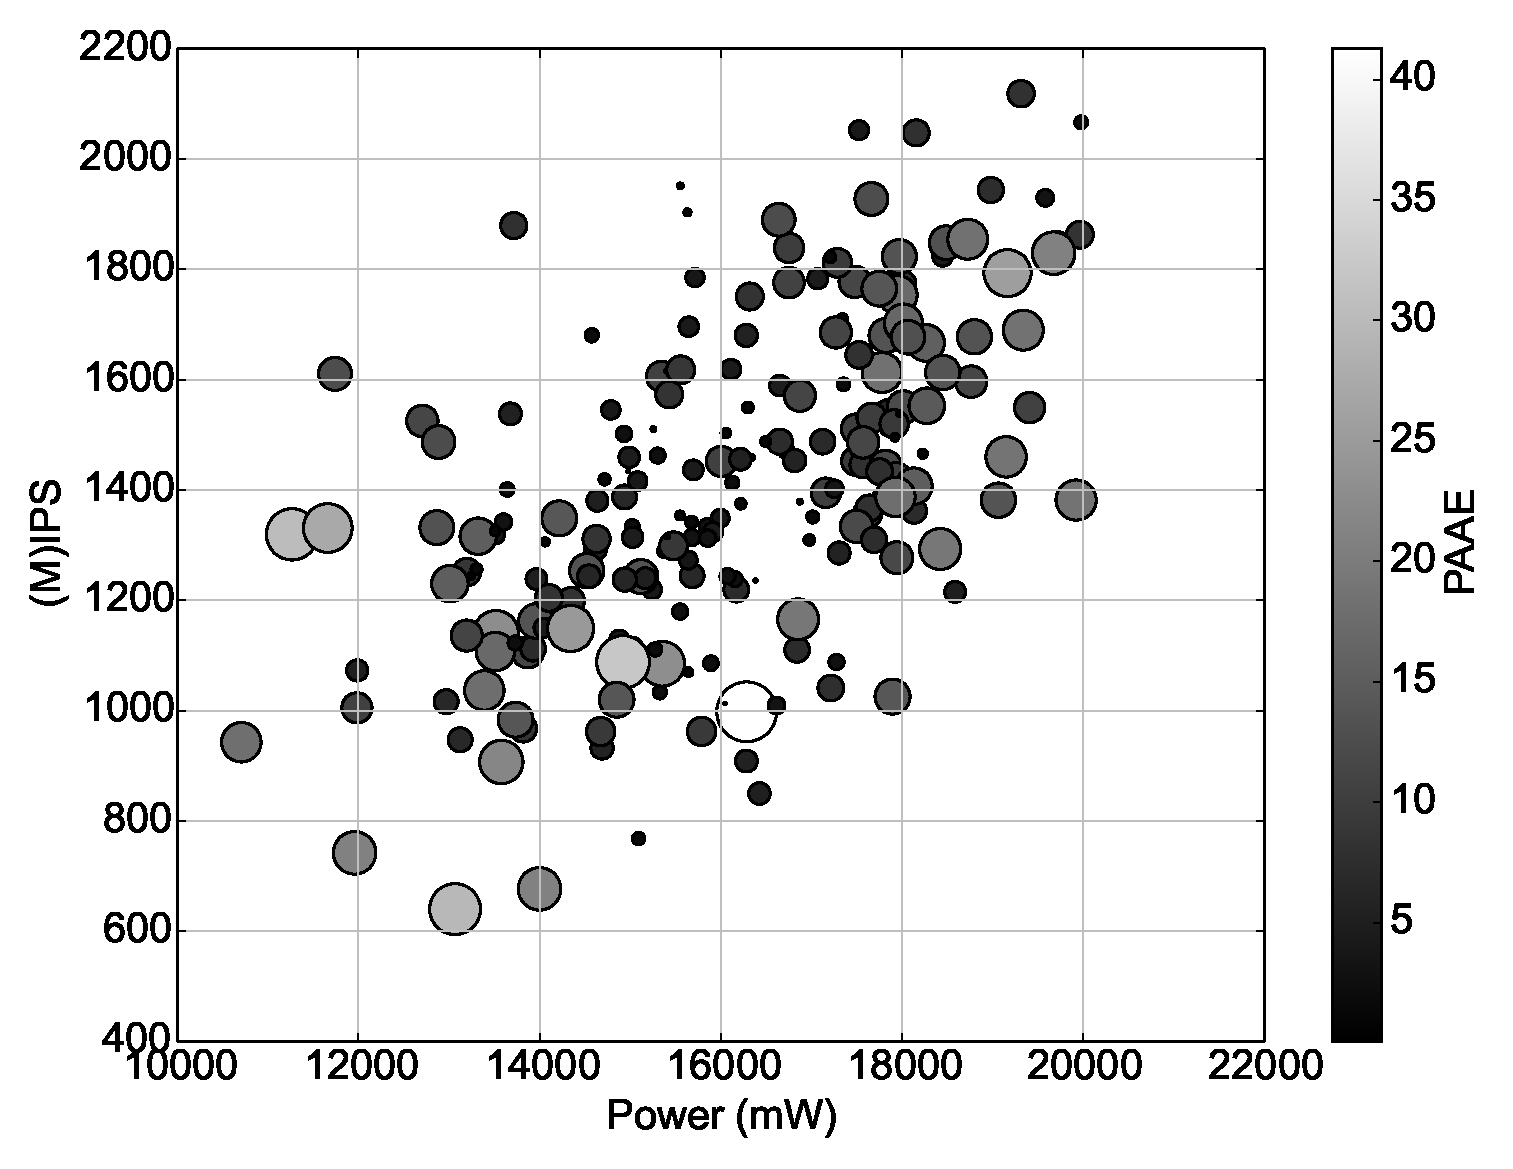
\includegraphics[width=\textwidth]{Chapter3/Figs/scatter/FFFN.eps}
        \caption{FFFN}
        \label{fig: FFFN}
    \end{subfigure}
    \begin{subfigure}{0.32\textwidth}
        \centering
        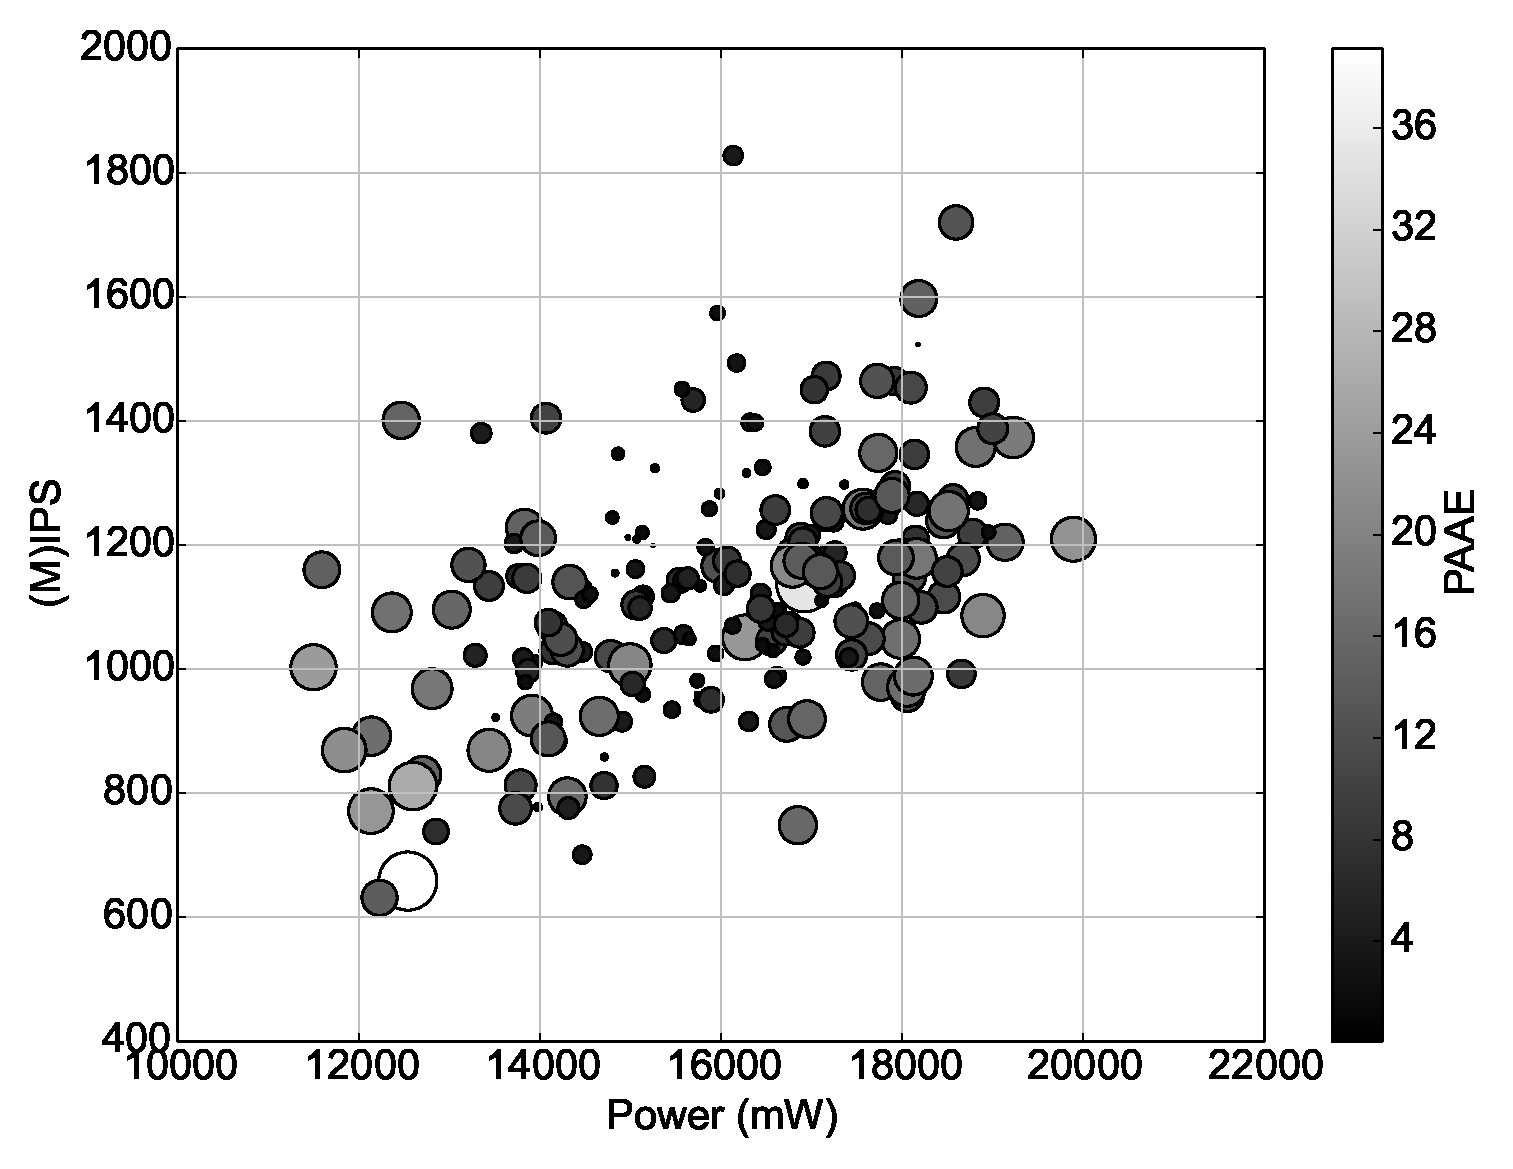
\includegraphics[width=\textwidth]{Chapter3/Figs/scatter/STFN.eps}
        \caption{STFN}  
        \label{fig: STFN}
    \end{subfigure}
    \caption[PAAE for workloads SSTN, FFFN and STFN on Intel]{\captitle{PAAE for workloads SSTN, FFFN and STFN on Intel.} Performance and power prediction error with change\_factor High.}
    \label{fig: REPPH result}
\end{figure*}

\looseness -1 Figure~\ref{fig: REPPH result} represents the performance on $y$-axis and
power on $x$-axis for multiprogrammed workloads SSTN, FFFN, and STFN on Intel architecture
with \textit{change\_factor} High. The radius of each circle is the maximum prediction
error, either power or performance (that is, $radius$ = $max$(PAAE\textsubscript{power},
PAAE\textsubscript{perf})). There exists multiple grayscale grading from low PAAE (black)
to high PAAE (white). Although the maximum PAAE shown is at the 50\% mark (the grayscale
in Figure~\ref{fig: SSTN} is up to 50\%), the number of error predictions with PAAE
greater than \SI{30}{\percent} is less than ten. For SSTN, FFFN and STFN, the average
error when predicting power (and performance) of \SI{9.7}{\percent} (\SI{3.3}{\percent}),
\SI{8.7}{\percent} (\SI{9.4}{\percent}) and \SI{8.4}{\percent} (\SI{6.7}{\percent}). This
behaviour is observed across all workloads.

\begin{figure}[t]
    \centering
    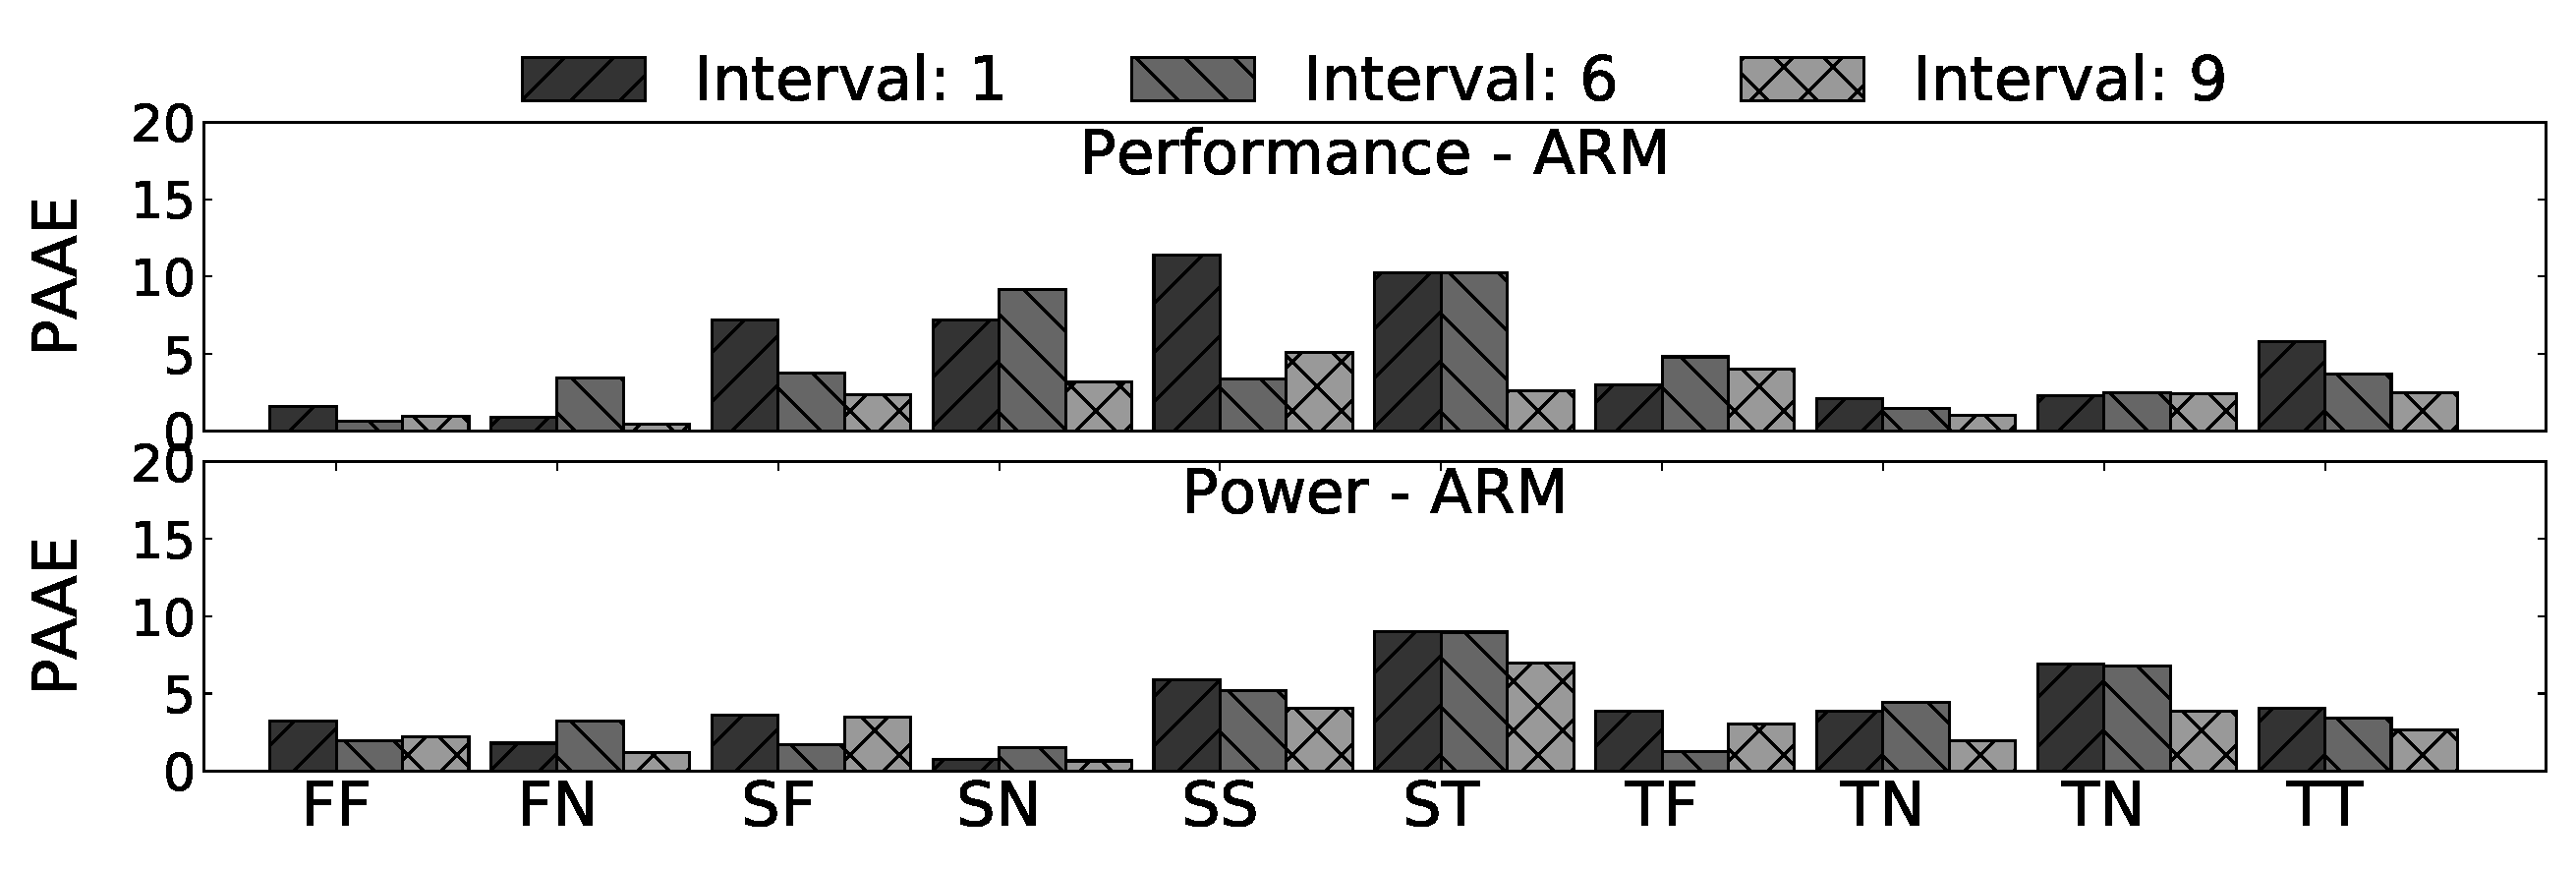
\includegraphics[width=\textwidth]{Chapter3/Figs/changefactor/summary-arm.eps}
    \caption[Average PAAE on ARM under different load\_change intervals]{\captitle{Average PAAE on ARM under different load\_change intervals.} Average PAAE when predicting power and performance for all workloads under different load\_change \texttt{intervals} for change\_factors Low, Mid and High. The $x$-axis shows multiprogrammed workloads.}
    \label{fig: armpowerperf}
\end{figure}

\begin{figure*}[htb!]
   \centering
    \begin{subfigure}{\textwidth}
        \centering
        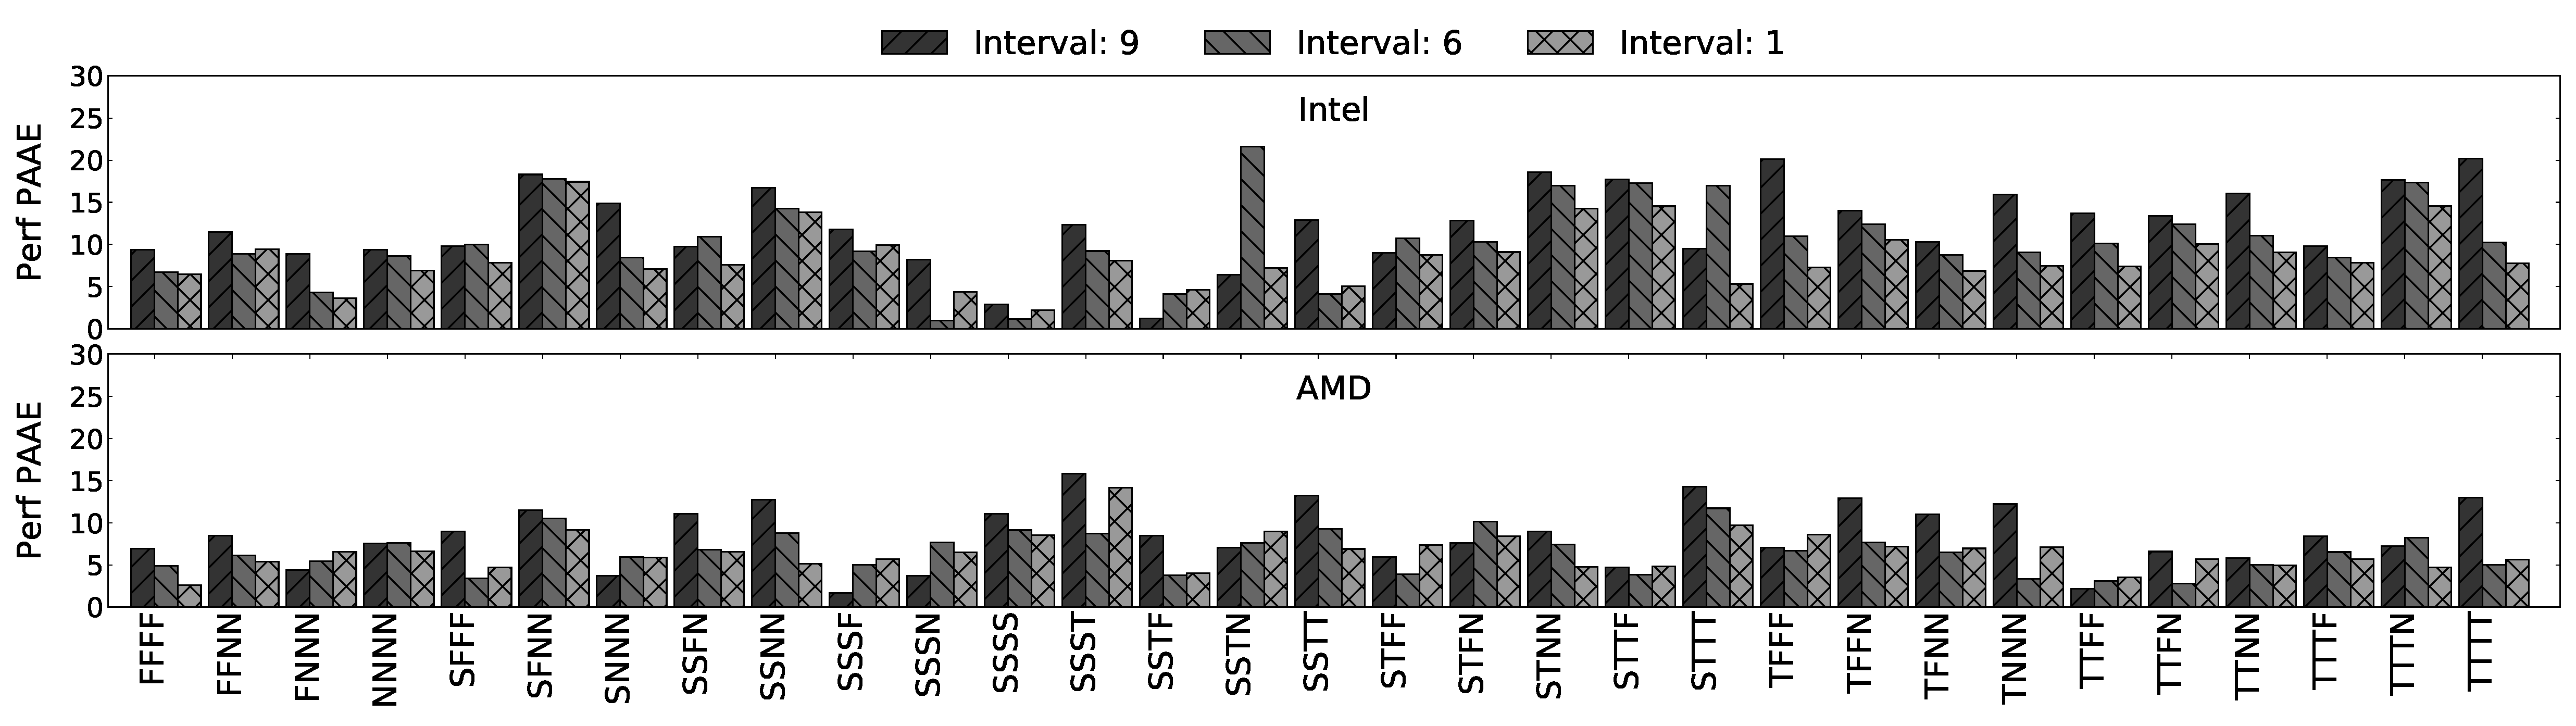
\includegraphics[width=\textwidth]{Chapter3/Figs/changefactor/summary_perf_intel_amd.eps}
        \caption{Performance}
        \label{fig: perfintelamd}
    \end{subfigure}
    \begin{subfigure}{\textwidth}
        \centering
        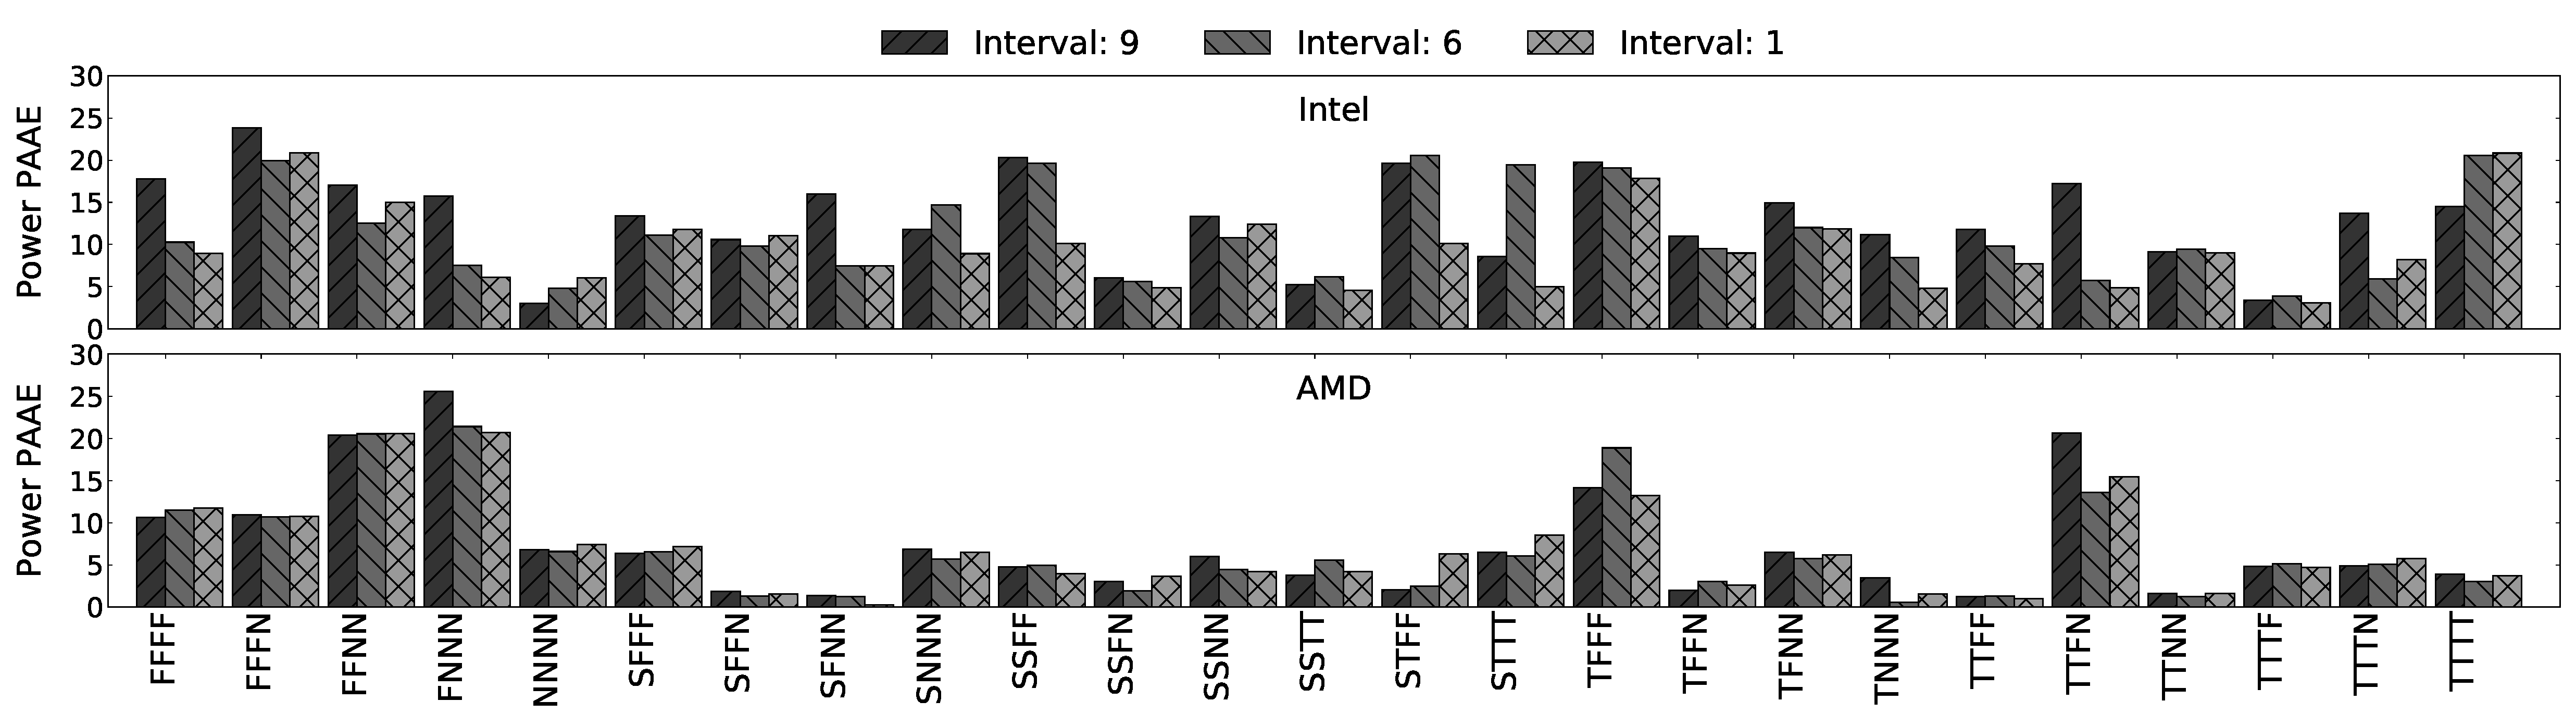
\includegraphics[width=\textwidth]{Chapter3/Figs/changefactor/summary_power_intel_amd.eps}
        \caption{Power}
        \label{fig: powerintelamd}
    \end{subfigure}
    \caption[Average PAAE on Intel and AMD under different load\_change intervals]{\captitle{Average PAAE on Intel and AMD under different load\_change intervals.} Average PAAE when predicting power and performance for all workloads under different load\_change \texttt{intervals} for change\_factors Low, Mid and High. The $x$-axis shows multiprogrammed workloads.}
    \label{fig: REPPH interval}
\end{figure*}


Figures~\ref{fig: REPPH interval} and~\ref{fig: armpowerperf} show the average PAAE for
each workload under different load\_change \texttt{intervals} on ARM and Intel/AMD when
predicting performance (Figure~\ref{fig: perfintelamd}) and power (Figure~\ref{fig:
powerintelamd}). Figures~\ref{fig: armpowerperf} and~\ref{fig: REPPH interval} are
separated because ARM has different number of cores. Across the three architectures,
faster (interval=1) load\_changes have \SI{3.5}{\percent} higher error compared to slower
(interval=9) load\_changes because of aggressive changes in load in short burst cause
numerous changes in configuration, thus leading to a higher error. On the other hand,
slower load\_changes lead to fewer changes in configuration, and have stable phases in
application behaviour.  Fortunately, data centres seldom want to jump from \SI{400}{\watt}
to \SI{600}{\watt} every second~\citep{6008553, Su:2014:POP:2742155.2742200}.
Table~\ref{tab: summarytable} summarises the result obtained when predicting power and
performance for load\_change interval \SI{1}{\second}, \SI{6}{\second} and
\SI{9}{\second}.

\begin{table}[ht]
\centering
\caption[Average PAAE for load\_change intervals]{\captitle{Average PAAE for load\_change intervals.} Power and performance error for load\_change intervals 1, 6 and 9 on Intel, AMD, and ARM.}
\begin{tabular}{@{}rrrrcrrrc@{}}\toprule
& \multicolumn{3}{c}{$Power$} & \phantom{abc}& \multicolumn{3}{c}{$Performance$} & \phantom{abc} \\
\cmidrule{2-4} \cmidrule{6-8} 
    $Interval$ & $\SI{1}{\second}$ & $\SI{6}{\second}$ & $\SI{9}{\second}$ && $\SI{1}{\second}$ & $\SI{6}{\second}$ & $\SI{9}{\second}$ \\ 
\midrule
    $Intel$     & \SI{11.1}{\percent} & \SI{7.3}{\percent}    & \SI{5.6}{\percent}  && \SI{11.4}{\percent} & \SI{10.6}{\percent}   & \SI{8.7}{\percent} \\
    $AMD$       & \SI{7.2}{\percent}  & \SI{6.9}{\percent}    & \SI{6.7}{\percent}  && \SI{8.5}{\percent}  & \SI{6.5}{\percent}    & \SI{6.5}{\percent} \\
    $ARM$       & \SI{4.2}{\percent} & \SI{3.8}{\percent}     & \SI{2.9}{\percent}  && \SI{5.1}{\percent}  & \SI{4.6}{\percent}    & \SI{2.4}{\percent} \\
\bottomrule
\end{tabular}
\label{tab: summarytable}
\end{table}

%\vspace*{2em}

\paragraph{Enabling Power/Performance Capping.} Determining a configuration to meet the
minimum performance (or not exceeding power consumption threshold) is usually done in an
iterative fashion (as in the RAPL driver on Intel processors~\citep{Intel}). A feedback
control loop is often used to determine the  configuration. If the power usage is above a
certain threshold, the configuration is lowered. On the other hand, if the power usage is
below a certain threshold, the configuration is increased to improve performance. In
contrast, we provide a single-step mechanism to select configurations.

\begin{figure}[t]
    \centering
    \includegraphics[width=\textwidth]{Chapter3/Figs/runtime/intel-runtime.eps}
    \caption[Responsiveness to power change on Intel]{\captitle{Responsiveness to power change on Intel.} Responsiveness to power capping for workload SSTT with constraint Random.}
    \label{fig: SSTT}
\end{figure}

Figure~\ref{fig: SSTT} shows the responsiveness to (dynamic) power capping for workload
\texttt{SSTT}, where the power capping limit is Random on Intel platform in the first 40
seconds. \texttt{SSTT} is composed of applications \emph{streamcluster}, \emph{lu.C},
\emph{bwaves} and \emph{soplex}. REPP changes DVFS states and meets the power target in
0.37 seconds on average, which is 3.6$\times$  faster than the iterative algorithm (used
by Intel RAPL). This time includes sampling interval, latency to predict at all DVFS state
and Cl-State and time to change DVFS state.  Moreover REPP, provides \SI{6}{\percent}
higher prediction accuracy. 






\section{Conclusion}
\label{subsec: conclusion}

This chapter introduced REPP, a procedure to predict performance and power at runtime for
single-core and \muc architectures using PMCs.  The technique includes a systematic method
to build multi linear regression models parametrised by hardware settings DVFS states and
Cl-States. The PMCs chosen to build the models are available across all major
architectures. 

We have shown that REPP is a scalable power and performance modelling, and prediction
technique to meet various user-defined criteria. The models have a fast deployment time
(less than 10 hours), involving a limited number of experiments on each architecture.
REPP's single-core and \muc models have been validated on each architecture using
benchmarks from SPEC CPU 2006, PARSEC 3.0, NAS and SPLASH2x. We perform real-machine
experimentation and use existing hardware support to profile the behaviour of
application's at runtime.

We validate REPP using several single threaded and multiprogrammed workloads with
average errors, respectively, on ARM, AMD and Intel architectures of \SI{7.1}{\percent},
\SI{9.0}{\percent}, \SI{7.1}{\percent} when predicting performance, and
\SI{6.0}{\percent}, \SI{6.5}{\percent}, \SI{8.1}{\percent} when predicting power
consumption.  Moreover, the single-step prediction technique provided by REPP is
3.6$\times$ faster than iterative algorithms. We argue that REPP can enable
operators to better control power and performance in modern data centres that include
server architectures with heterogeneous processing capabilities. 
